\documentclass[12pt,a4paper]{report}

\usepackage{ragged2e}
\usepackage{setspace}
\usepackage[T1]{fontenc}
\usepackage{graphicx}
\graphicspath{{./}{./overleaf_figures/}{./results/}{./sample_ad_media/}}
\usepackage{url}
\usepackage{times}
\usepackage{hyperref}
\usepackage[nottoc,notlot,notlof]{tocbibind}
\usepackage{amsmath}
\usepackage{amssymb}
\usepackage{caption}
\usepackage{subcaption}
\usepackage{booktabs}
\usepackage{array}
\usepackage{float}
\usepackage{listings}
\usepackage{xcolor}
\usepackage[left=3.5cm,top=2.0cm,right=2.5cm,bottom=2.5cm]{geometry}

\setcounter{tocdepth}{2}

\raggedbottom
\widowpenalty=10000
\clubpenalty=10000
\brokenpenalty=10000

\renewcommand{\topfraction}{0.90}
\renewcommand{\bottomfraction}{0.85}
\renewcommand{\textfraction}{0.10}
\renewcommand{\floatpagefraction}{0.75}

\renewcommand{\baselinestretch}{1.20}
\renewcommand{\bibname}{References}
\renewcommand\listfigurename{\centering {List of Figures}}
\renewcommand\listtablename{\centering{List of Tables}}
\hypersetup{hidelinks}

\definecolor{codegray}{rgb}{0.5,0.5,0.5}
\definecolor{codepurple}{rgb}{0.58,0,0.82}
\definecolor{backcolour}{rgb}{0.97,0.98,0.99}

\lstdefinestyle{mystyle}{
    backgroundcolor=\color{backcolour},   
    commentstyle=\color{codegray},
    keywordstyle=\color{blue},
    numberstyle=\tiny\color{codegray},
    stringstyle=\color{codepurple},
    basicstyle=\ttfamily\scriptsize,
    breakatwhitespace=false,         
    breaklines=true,                 
    captionpos=b,                    
    keepspaces=true,                 
    numbers=left,                    
    numbersep=4pt,                  
    tabsize=2
}
\lstset{style=mystyle}

\begin{document}

\justifying
\setlength{\emergencystretch}{3em}
\tolerance=2000
\hbadness=10000

% ============================================================
% TITLE PAGE
% ============================================================

\begin{titlepage}
\begin{center}

\vspace*{0.2cm}

{\LARGE \textbf{SafeAd AI: Multimodal Trust and Safety Framework for Advertisement Moderation}}\\[0.4cm]

{\Large \textbf{A Project Report}}\\[0.2cm]

\large \textit{Submitted to the APJ Abdul Kalam Technological University}\\[0.1cm]

\large \textit{in partial fulfillment of requirements for the award of degree}\\[0.5cm]

{\Large \textbf{Bachelor of Technology}}\\[0.1cm]

\large {in}\\[0.1cm]

{\Large \textbf{Computer Science and Engineering}}\\[0.1cm]

{\large \textbf{(Artificial Intelligence)}}\\[0.2cm]

\large \textit{by}\\[0.2cm]

{\large \textbf{\scshape Joseph Benedict} \textbf{\textit{(B23CS2136, KTU Reg No: MBT23CA036)}}}\\

{\large \textbf{\scshape Juwel Jokesh} \textbf{\textit{(B23CS2138, KTU Reg No: MBT23CA038)}}}\\

{\large \textbf{\scshape R D Sourav} \textbf{\textit{(B23CS2151, KTU Reg No: MBT23CA052)}}}\\

{\large \textbf{\scshape Sooraj Jose George} \textbf{\textit{(B23CS2160, KTU Reg No: MBT23CA059)}}}\\[0.5cm]

\IfFileExists{mbcetlogo.png}{\centerline{
\includegraphics[width=4.0cm]{mbcetlogo.png}}}{\vspace{4.0cm}}

\vspace*{0.4cm}

{\bf \large Department of Computer Science and Engineering}\\

{\bf \large Mar Baselios College of Engineering and Technology}\\

{\large Thiruvananthapuram -- 695015}\\[0.2cm]

{\large OCTOBER 2026}

\end{center}
\end{titlepage}

% ============================================================
% CERTIFICATE
% ============================================================

\newpage
\thispagestyle{empty}

\begin{center}
{\bf \large Department of Computer Science and Engineering}\\[0.1cm]
{\bf \large Mar Baselios College of Engineering and Technology}\\[0.1cm]
{\large Thiruvananthapuram -- 695015}\\[0.4cm]

\IfFileExists{mbcetlogo.png}{\centerline{
\includegraphics[width=3.0cm]{mbcetlogo.png}}}{\vspace{3.0cm}}

\vspace{0.4cm}
{\bf \Large CERTIFICATE}
\end{center}

\noindent This is to certify that the project report entitled \textbf{``SafeAd AI: Multimodal Trust and Safety Framework for Advertisement Moderation''} is a bonafide record of the work carried out by \textbf{Joseph Benedict (MBT23CA036)}, \textbf{Juwel Jokesh (MBT23CA038)}, \textbf{R D Sourav (MBT23CA052)}, and \textbf{Sooraj Jose George (MBT23CA059)} in partial fulfillment of the requirements for the award of the degree of \textbf{Bachelor of Technology in Computer Science and Engineering (Artificial Intelligence)} of the \textbf{APJ Abdul Kalam Technological University} during the academic year 2025--2026.

\vspace{1.8cm}

\noindent
\begin{tabular}{@{}p{5.0cm}p{4.5cm}p{5.5cm}@{}}
\textbf{Ms. Gayathri K. S.} & \textbf{Dr. Neena Raj N. R.} & \textbf{Dr. Anne Dickson} \\
Assistant Professor & Associate Professor & Professor and Head \\
Project Guide & Project Coordinator & Dept. of CSE \\
MBCET, Thiruvananthapuram & MBCET, Thiruvananthapuram & MBCET, Thiruvananthapuram
\end{tabular}

% ============================================================
% DECLARATION
% ============================================================

\newpage
\thispagestyle{empty}

\begin{center}
{\bf \Large DECLARATION}
\end{center}

\vspace{0.8cm}

\noindent We hereby declare that the project report entitled \textbf{``SafeAd AI: Multimodal Trust and Safety Framework for Advertisement Moderation''}, submitted to the \textbf{APJ Abdul Kalam Technological University} in partial fulfillment of the requirements for the award of the Degree of \textbf{Bachelor of Technology in Computer Science and Engineering (Artificial Intelligence)}, is a record of original work done by us under the supervision and guidance of \textbf{Ms. Gayathri K. S.}, Assistant Professor, Department of Computer Science and Engineering, Mar Baselios College of Engineering and Technology, Thiruvananthapuram.

\vspace{0.4cm}

\noindent We further declare that this report has not previously formed the basis for the award of any degree, diploma, fellowship, or associateship of any other university or institute of higher learning.

\vspace{1.8cm}

\noindent
\begin{tabular}{@{}p{7.5cm}p{7.5cm}@{}}
\textbf{Joseph Benedict} (MBT23CA036) & \textbf{Juwel Jokesh} (MBT23CA038) \\[1.2cm]
\textbf{R D Sourav} (MBT23CA052) & \textbf{Sooraj Jose George} (MBT23CA059)
\end{tabular}

\vspace{1.0cm}
\noindent Thiruvananthapuram \\
\noindent Date: 30-10-2026

% ============================================================
% ACKNOWLEDGEMENT
% ============================================================

\newpage
\thispagestyle{empty}

\begin{center}
{\bf \Large ACKNOWLEDGEMENT}
\end{center}

\vspace{0.6cm}

\noindent We express our deepest gratitude to the Almighty for the grace, wisdom, and perseverance bestowed upon us throughout the execution of this research endeavor.

\vspace{0.3cm}

\noindent We extend our sincere gratitude to \textbf{Dr. Abraham T. Mathew}, Principal, Mar Baselios College of Engineering and Technology, for providing the institutional infrastructure, research computing environment, and high-performance computing facilities necessary to realize this project.

\vspace{0.3cm}

\noindent We convey our profound appreciation to \textbf{Dr. Anne Dickson}, Professor and Head of the Department of Computer Science and Engineering, for her administrative support, constructive advice, and scholarly encouragement.

\vspace{0.3cm}

\noindent We record our deep debt of gratitude to our project guide, \textbf{Ms. Gayathri K. S.}, Assistant Professor, Department of Computer Science and Engineering, whose meticulous technical guidance, critical insights, and unwavering dedication shaped the scientific direction of this research. We are also immensely grateful to our Project Coordinator, \textbf{Dr. Neena Raj N. R.}, Associate Professor, Department of Computer Science and Engineering, for her continuous coordination, structured reviews, and rigorous academic feedback.

\vspace{0.3cm}

\noindent Finally, we express heartfelt thanks to our families, fellow students, and academic peers whose constant encouragement, patience, and support sustained us throughout this intensive endeavor.

\vspace{1.0cm}
\noindent
\textbf{Joseph Benedict}\\
\textbf{Juwel Jokesh}\\
\textbf{R D Sourav}\\
\textbf{Sooraj Jose George}

% ============================================================
% ABSTRACT
% ============================================================

\newpage
\pagenumbering{roman}
\setcounter{page}{1}

\begin{center}
{\bf \Large ABSTRACT}
\end{center}

\vspace{0.5cm}

\noindent The rapid expansion of programmatic digital advertising networks has outpaced conventional reactive moderation systems, allowing deceptive, sexually suggestive, and age-inappropriate content to bypass safety guardrails. Modern adversarial advertisements exploit cross-modal semantic concealment, wherein benign visual assets are combined with predatory audio narrations or obscured typographic overlays, deliberately circumventing single-modality content filters. 

To overcome these critical security vulnerabilities, this project presents \textbf{SafeAd AI (SAFE-VISION)}, an end-to-end, pre-publication multimodal trust and safety framework designed for real-time advertisement verification and age-aware content dispatching. The framework implements a synchronized dual-engine architecture: (1) an automated multimodal content moderation engine that ingests video keyframes, optical character recognition (OCR) typography, and automatic speech recognition (ASR) audio transcripts to evaluate cross-modal policy compliance; and (2) a biometric age assurance and facial verification subsystem that enforces regulatory delivery boundaries across four distinct statutory tiers: \texttt{SAFE\_FOR\_ALL}, \texttt{SAFE\_14\_PLUS}, \texttt{SAFE\_18\_PLUS}, and \texttt{UNSAFE\_FOR\_ALL}.

The content moderation engine extracts high-dimensional representations across video kinetics (VideoMAE), adult visual concepts (Falcon NSFW ViT), textual semantics (RoBERTa and DeBERTa-v3), and commercial claim risk heuristics. In development benchmark evaluations ($N=194$), a learned late-fusion Random Forest achieved an overall 5-fold cross-validation accuracy of $44.33\%$ with a macro-F1 of $0.4496$. Rigorous error profiling revealed that generic visual safety guardrails (such as Llama Guard 3 Vision) fail on $80.0\%$ of diagnostic ad cohorts due to severe commercial concept blindness. To resolve this semantic bottleneck, the framework integrates Qwen3-VL-8B-Instruct, an 8-billion parameter vision-language foundation model with ad-policy prompt alignment, coupled with a hierarchical policy-aware late-fusion protocol (Strategy~D).

On a strictly independent, held-out test cohort of 27 verified advertisement assets evaluated on an NVIDIA A100 GPU without ground-truth leakage or rule post-tuning, Qwen3-VL and Hierarchical Fusion achieved $66.7\%$ four-class accuracy, successfully eliminating all severe false acceptances ($0.0\%$ false acceptance rate) and achieving a flawless $100.0\%$ recall on strictly prohibited content. The companion biometric subsystem combines dual-scale MiniFASNet with 2D Fast Fourier Transform (FFT) moir\'{e} analysis for Presentation Attack Detection ($93.0\%$ replay attack detection accuracy) and ArcFace embedding verification ($96.50\%$ True Accept Rate at $0.1\%$ False Accept Rate), guaranteeing that age-restricted advertisements are strictly inaccessible to minors. The resulting system bridges the divide between regulatory advertising standards and real-time automated enforcement.

\vspace{0.4cm}
\noindent \textbf{Keywords:} Multimodal Content Moderation, Trust and Safety, Vision-Language Models, Policy Enforcement, Late Fusion, Presentation Attack Detection, Biometric Age Assurance.

% ============================================================
% TOC, LOF, LOT
% ============================================================

\newpage
\tableofcontents

\newpage
\listoffigures

\newpage
\listoftables

\newpage
\pagenumbering{arabic}
\setcounter{page}{1}


\chapter{Introduction}
\label{ch:intro}

\section{Background and Industrial Context}
The digital advertising ecosystem has shifted from manually negotiated direct placements to fully automated, programmatic ad exchanges. In modern programmatic ad networks, bidding decisions, creative matching, and asset rendering take place within milliseconds across billions of daily impressions. According to global digital market analyses, online advertising expenditures exceeded \$600 billion globally in 2024, with video and rich media capturing dominant market share across social platforms such as Instagram, YouTube, and Meta.

While programmatic infrastructure delivers unmatched targeting efficiency, it has introduced severe vulnerabilities into platform trust and safety architectures. Traditional content moderation systems were designed primarily for post-publication, user-reported takedowns. In a real-time programmatic ad exchange, however, a single malicious or age-inappropriate creative asset can be delivered to millions of adolescent and vulnerable viewers before user flags trigger review. The pre-publication window represents the sole point of leverage where predatory, fraudulent, and non-compliant material can be intercepted before public harm occurs.

\section{The Threat Landscape: Cross-Modal Concealment Tactics}
Digital threat actors and unscrupulous advertisers have developed sophisticated adversarial strategies to bypass conventional single-modality content safety filters:
\begin{enumerate}
    \item \textbf{Benign Visual Scene Pairing:} An advertisement presents visually harmless imagery---such as an innocuous domestic setting or animated figures---which easily passes visual classifiers. However, the synchronized audio track delivers predatory investment pitches or unauthorized financial schemes.
    \item \textbf{Typographic and OCR Evasion:} Critical deceptive claims, counterfeit contact details, or prohibited keywords are embedded within video frames using complex stylized fonts, low-contrast text backgrounds, or brief flash-frame durations (under 300~ms), evading standard OCR engines.
    \item \textbf{Regulatory Disclaimer Obfuscation:} Advertisements for high-risk financial instruments, sports betting, or alcohol frequently render statutory warnings in microscopic font sizes at the extreme periphery of the screen for sub-second durations.
    \item \textbf{Kinetic Concealment:} Malicious actors inject prohibited violence or adult content only within isolated, high-motion transition frames that evade sparse uniform keyframe extraction algorithms.
\end{enumerate}

Existing automated moderation pipelines rely predominantly on unimodal filters operating in silos. These architectures cannot recognize cross-modal irony, sarcastic juxtapositions, or context-dependent statutory violations where no individual modality contains explicit obscenity, yet their multimodal synthesis produces an unlawful advertisement.

\section{The Structural Disconnection: Content Safety vs. Viewer Demographics}
A fundamental limitation of contemporary ad safety infrastructure is the complete decoupling between content moderation classifications and viewer demographic characteristics. Standard moderation systems assign static binary ``safe'' versus ``unsafe'' flags without considering the age, developmental maturity, or legal protections of the intended recipient.

Statutory frameworks across international jurisdictions, including COPPA in the United States, the EU Digital Services Act (DSA), and the ASCI Code, mandate strict age gating for sensitive product categories. Products such as alcoholic beverages, sports wagering, mature video games, and cosmetic procedures are entirely lawful for adult consumers ($18+$ years) but legally prohibited from distribution to minors. When a moderation system is blind to viewer demographics, platforms face an unacceptable trade-off: either aggressively censor lawful adult commerce, causing immense publisher revenue loss, or adopt permissive thresholds that systematically expose adolescents and children to hazardous material.

Furthermore, conventional client-side age verification mechanisms rely on self-reported birthdates, unverified profile checkboxes, or easily forgeable digital forms. Minors routinely bypass these weak checkpoints. A robust advertising trust and safety framework must unite pre-publication multimodal asset moderation with spoof-resistant biometric age assurance.

\section{The SafeAd AI Vision and Core Paradigms}
To resolve these structural vulnerabilities, this project presents \textbf{SafeAd AI (SAFE-VISION)}, an end-to-end multimodal trust and safety framework engineered specifically for pre-publication advertisement verification and age-aware content dispatching:
\begin{enumerate}
    \item \textbf{Proactive Pre-Publication Interception:} Moving beyond post-publication reactive moderation, SafeAd AI analyzes full video, image, typographic, and acoustic assets in real time prior to programmatic auction approval.
    \item \textbf{Deep Multimodal Cross-Modal Fusion:} The framework combines specialized neural representations (video motion dynamics, adult visual features, OCR text embeddings, and audio transcripts) through learned late fusion and vision-language foundation models (VLMs) equipped with structured policy guardrails.
    \item \textbf{Synchronized Biometric Age Gating:} The framework couples creative asset classification with a biometric client-side age assurance pipeline that combines deep face verification (ArcFace), Presentation Attack Detection (MiniFASNet and 2D FFT Moir\'{e} filtering), and ID document OCR.
\end{enumerate}

\section{Detailed Problem Statement and Mathematical Objectives}
Let an incoming advertisement asset be denoted by the multimodal tuple $\mathcal{M} = (\mathbf{I}, \mathbf{A}, \mathbf{T}, \mathbf{X}, \mathbf{M}_{\text{meta}})$, where $\mathbf{I}$ represents video keyframes, $\mathbf{A}$ is the raw audio stream, $\mathbf{T}$ denotes on-screen text extracted via OCR, $\mathbf{X}$ is the speech transcript, and $\mathbf{M}_{\text{meta}}$ represents advertiser metadata.

The primary objective of the multimodal moderation engine $\Phi$ is to learn a mapping:
\begin{equation}
\Phi: \mathcal{M} \longrightarrow \left( \hat{y}_{\text{pred}}, S_{\text{risk}}, \mathbf{e}, \mathbf{c} \right)
\end{equation}
where $\hat{y}_{\text{pred}} \in \mathcal{C} = \{\texttt{SAFE\_FOR\_ALL}, \texttt{SAFE\_14\_PLUS}, \texttt{SAFE\_18\_PLUS}, \texttt{UNSAFE\_FOR\_ALL}\}$, $S_{\text{risk}} \in [0.0, 100.0]$ is the continuous composite hazard score, $\mathbf{e}$ is a natural language policy rationale, and $\mathbf{c} \in [0.0, 1.0]^4$ is a calibrated posterior probability distribution.

Simultaneously, the biometric recipient verification engine $\Psi$ maps client visual telemetry $(D_{\text{ID}}, K_{\text{live}})$ to a verified viewer demographic $\hat{g}_{\text{user}} \in \{\texttt{UNDER\_14}, \texttt{AGE\_14\_TO\_17}, \texttt{AGE\_18\_PLUS}\}$, subject to anti-spoofing liveness verification. The final dispatching operator $\mathcal{D}(\hat{y}_{\text{pred}}, \hat{g}_{\text{user}})$ ensures that no asset is delivered to a viewer whose age bracket falls below the statutory threshold of $\hat{y}_{\text{pred}}$, achieving a zero false-acceptance rate for strictly prohibited and underage exposures.

\section{Project Objectives}
The specific scientific and engineering objectives of this project are:
\begin{enumerate}
    \item \textbf{Multimodal Ingestion and Adaptive Sampling:} Design an automated media processing pipeline that performs adaptive keyframe selection using Farneb\"{a}ck dense optical flow, robust typographic text extraction via CLAHE and EasyOCR, and speech transcription using Whisper.
    \item \textbf{Specialized Feature Representation:} Extract dense semantic embeddings across modalities using specialized neural architectures, including Falcon NSFW ViT for adult visual concepts, VideoMAE for violent motion dynamics, and RoBERTa/DeBERTa for textual toxicity.
    \item \textbf{Learned and Foundation Model Fusion:} Implement and evaluate both a learned late-fusion Random Forest classifier and an advanced Vision-Language Foundation Model (Qwen3-VL-8B-Instruct) governed by hierarchical safety veto rules (Strategy~D).
    \item \textbf{Independent Held-Out Benchmark Evaluation:} Subject the complete pipeline to rigorous, leak-free validation on an independent held-out test cohort ($N=27$) executed on an NVIDIA A100 GPU, documenting full confusion matrices and forensic failure modes.
    \item \textbf{Biometric Age Assurance and Anti-Spoofing:} Develop a companion biometric client subsystem combining InsightFace ArcFace for identity verification, a dual-scale MiniFASNet neural ensemble with 2D FFT frequency analysis for Presentation Attack Detection, and automated ID document OCR parsing.
    \item \textbf{Explainable Dashboard and Audit Trail:} Deploy a full-stack web application featuring an advertiser submission portal, an administrative compliance review interface, and an immutable JSON audit log.
\end{enumerate}

\section{Report Organization}
The remainder of this report is organized as follows: Chapter~\ref{ch:lit_review} surveys related literature; Chapter~\ref{ch:policy} formulates the mathematical model and four-tier policy taxonomy; Chapter~\ref{ch:architecture} details the system architecture and UML modeling; Chapter~\ref{ch:methodology} elaborates on feature extraction, fusion algorithms, and biometric PAD; Chapter~\ref{ch:results} reports empirical findings and forensic error audits; and Chapter~\ref{ch:conclusion} presents conclusions and future scope.


\chapter{Literature Review}
\label{ch:lit_review}

\section{Evolution of Digital Content Moderation Architectures}
Automated digital content moderation has evolved through three distinct technological paradigms over the past two decades. The earliest architectures relied heavily on rule-based keyword blacklists, regular expression pattern matching, and visual perceptual hashing algorithms such as PhotoDNA and perceptual hashing (pHash)~\cite{kiela2020hateful}. While computationally lightweight and deterministic, these systems suffered from extreme fragility. Malicious users easily evaded text filters through leetspeak substitutions, zero-width spaces, and phonetic transliterations, while simple image affine transformations, cropping, and color jittering defeated perceptual hashing techniques.

The second paradigm emerged with deep convolutional neural networks (CNNs) and transformer-based language representations. Models such as ResNet, EfficientNet, and BERT enabled semantic classification of text toxicity and visual obscenity~\cite{devlin2018bert}. Specialized vision models, including Falcon NSFW ViT, introduced fine-grained classification of sexually explicit imagery. Similarly, temporal video architectures such as VideoMAE~\cite{tong2022videomae} enabled the detection of violent combat and kinetic anomalies across consecutive video frames. Despite their high accuracy on isolated tasks, these models operated within unimodal silos, rendering them blind to cross-modal relationships.

The third paradigm centers on multimodal foundation models. Systems like CLIP~\cite{radford2021learning} demonstrated the power of contrastive visual-language pre-training for zero-shot classification. However, standard foundation models are trained on general internet distributions and frequently fail to interpret domain-specific commercial advertising policies, deceptive marketing claims, or fine-grained statutory age restrictions.

\section{Implicit Semantics and Cross-Modal Concealment}
A major vulnerability in automated trust and safety systems is implicit semantics, including sarcasm, double entendre, and cross-modal discordance. The Facebook Hateful Memes Benchmark introduced by Kiela et al.~\cite{kiela2020hateful} empirically established that unimodal state-of-the-art architectures degrade significantly when evaluating multimodal assets where neither image nor text is harmful independently, but their juxtaposition forms a policy violation.

In digital advertising, adversarial creators employ analogous techniques to bypass pre-publication review. An advertisement promoting unauthorized pharmaceutical supplements may display an image of wholesome agricultural produce while embedding deceptive health claims entirely within the audio narration. Conversely, an advertisement for adult dating services may pair clean stock photography with sexually suggestive double entendres in the on-screen typography. Resolving such cross-modal concealment requires joint semantic fusion mechanisms capable of cross-referencing acoustic, visual, and typographic features simultaneously~\cite{sharma2022survey}.

\section{Policy-Aligned Commercial Advertisement Moderation}
While generic content moderation focuses on extreme harms such as terrorism and hate speech, commercial advertisement moderation operates under highly nuanced statutory standards. Organizations such as the Federal Trade Commission (FTC) in the United States and the Advertising Standards Council of India (ASCI) enforce strict guidelines governing truth in advertising, substantiation of commercial claims, conspicuous disclosure of disclaimers, and restriction of age-sensitive goods~\cite{ftc2020guides, asci2021code}.

Automated systems must therefore evaluate legal and commercial dimensions beyond vulgarity. Commercial deception detection requires cross-referencing extracted OCR claims against recognized fraud patterns. In video advertising, temporal dynamics play a crucial role. Studies by Hussein et al.~\cite{hussein2020multimodal} demonstrate that video moderation must incorporate keyframe extraction algorithms capable of capturing rapid visual transitions without incurring the computational overhead of decoding every frame.

\section{Vision-Language Foundation Models and Safety Guardrails}
The advent of autoregressive Vision-Language Models (VLMs), such as Llama Guard 3 Vision~\cite{metallama2024} and Qwen-VL~\cite{bai2023qwen}, has opened new frontiers for automated policy enforcement. Llama Guard 3 Vision was introduced specifically as an open-weights safety guardrail designed to identify safety violations across standardized taxonomy categories.

However, empirical investigations reveal critical domain limitations when generic safety VLMs are applied directly to commercial advertising moderation. Because safety guardrails are fine-tuned on extreme web safety benchmarks, they suffer from severe commercial concept blindness. They lack the granular taxonomy required to differentiate between benign consumer products, restricted adult commerce (such as alcohol, casino gambling, or adult dating), and deceptive financial frauds. Adapting VLMs for commercial trust and safety requires structured prompt engineering, policy-aligned chain-of-thought elicitation, and integration with specialized downstream discriminative detectors.

\section{Multimodal Fusion Paradigms: Early, Late, and Intermediate}
In multimodal machine learning, the fusion paradigm dictates how representations from disparate modalities are combined:
\begin{itemize}
    \item \textbf{Early Fusion (Feature-Level):} Raw sensory features or low-level embedding vectors are concatenated into a single joint vector prior to classification. While early fusion captures low-level cross-modal correlations, it suffers from the curse of dimensionality and is highly vulnerable to missing modalities.
    \item \textbf{Intermediate Fusion (Cross-Attention):} Modalities interact through intermediate cross-attention layers. While expressive, cross-attention networks demand massive paired training corpora and substantial computational resources.
    \item \textbf{Late Fusion (Decision-Level):} Specialized unimodal models generate independent posterior probability distributions, which are subsequently combined via learned meta-classifiers or heuristic policy rules~\cite{gadzicki2020review}.
\end{itemize}

Late fusion provides superior resilience in production advertising networks. It allows modular replacement of individual detector components, operates gracefully when specific media streams are absent, and supports deterministic hierarchical override rules (such as zero-tolerance safety vetoes).

\section{Biometrics and Presentation Attack Detection (PAD)}
Enforcing age-aware advertising policies necessitates verifiable client-side demographic assurance. Machine learning approaches to demographic assurance leverage facial analysis, wherein deep feature extractors estimate chronological age brackets from facial morphology~\cite{rothe2018dex}. To provide statutory compliance, modern systems implement hybrid identity verification, wherein facial embeddings extracted via deep metric learning (e.g., ArcFace~\cite{deng2019arcface}) are compared against digitized national identity documents.

Any biometric verification system deployed on consumer webcams is susceptible to Presentation Attacks (print attacks and screen replays)~\cite{yu2020nasfas}. Standard 2D Presentation Attack Detection architectures utilize lightweight convolutional networks, such as MiniFASNet~\cite{zhang2020minifasnet}, trained on multi-scale spatial features. In addition, digital screens display periodic pixel grids that generate high-frequency moir\'{e} interference patterns under camera re-capture. Applying 2D Fast Fourier Transforms (FFT) enables real-time isolation of artificial high-frequency energy spikes indicative of screen replay spoofing.

\section{Comparative Literature Summary and Research Gaps}
Table~\ref{tab:lit_comparison} provides a comparative summary of existing content moderation and biometric verification architectures.

\begin{table}[htbp]
\centering
\caption{Comprehensive Comparison of Content Moderation and Safety Architectures}
\label{tab:lit_comparison}
\scriptsize
\begin{tabular}{@{}p{2.6cm}p{1.0cm}p{2.6cm}p{2.6cm}p{5.5cm}@{}}
\toprule
\textbf{Study / Architecture} & \textbf{Year} & \textbf{Target Domain} & \textbf{Modalities} & \textbf{Key Capabilities and Critical Gaps} \\
\midrule
Kiela et al.~\cite{kiela2020hateful} & 2020 & Social Memes & Image + Text & Introduced Hateful Memes Benchmark; lacks audio, video kinetics, and ad policies. \\
Tong et al.~\cite{tong2022videomae} & 2022 & Action Recognition & Video & Self-supervised video pre-training; computationally intensive, no audio/text integration. \\
Falcon NSFW ViT~\cite{falcon2023nsfw} & 2023 & Visual Safety & Image & High-precision adult imagery detection; binary output, completely blind to text/audio context. \\
Meta Llama Guard 3~\cite{metallama2024} & 2024 & LLM Safety & Image + Text & Open safety guardrail; suffers $80\%$ failure on commercial ad fraud and adult retail. \\
Bai et al. (Qwen-VL)~\cite{bai2023qwen} & 2023 & Multimodal VLM & Image + Text & Strong visual reasoning; requires policy prompt alignment and safety veto wrappers. \\
Deng et al. (ArcFace)~\cite{deng2019arcface} & 2019 & Face Recognition & Facial Images & Angular margin loss for face matching; requires companion PAD to prevent replay spoofing. \\
Zhang et al. (MiniFASNet)~\cite{zhang2020minifasnet} & 2020 & Face Anti-Spoofing & Video Streams & Lightweight mobile PAD network; vulnerable to high-definition screen replays without FFT analysis. \\
\bottomrule
\end{tabular}
\end{table}

This review reveals five critical research gaps: (1) unimodal evaluation blindness, (2) commercial concept blindness of generic foundation models, (3) decoupling of content safety from viewer demographics, (4) vulnerability to replay presentation attacks, and (5) lack of explainable, tamper-evident audit trails. SafeAd AI is engineered specifically to bridge these five gaps.


\chapter{Problem Formulation and Policy Framework}
\label{ch:policy}

\section{Mathematical System Formulation}
Let the multimodal creative asset space be denoted by the tuple:
\begin{equation}
\mathcal{M} = \left( \mathbf{I}, \mathbf{A}, \mathbf{T}, \mathbf{X}, \mathbf{M}_{\text{meta}} \right)
\end{equation}
where $\mathbf{I} = \{I_1, I_2, \dots, I_K\}$ represents $K$ sampled video keyframes, $\mathbf{A} \in \mathbb{R}^{S}$ is the 16~kHz mono PCM audio track, $\mathbf{T}$ is the on-screen text extracted via OCR, $\mathbf{X}$ is the speech transcript from Whisper ASR, and $\mathbf{M}_{\text{meta}}$ represents advertiser metadata.

The pre-publication moderation engine $\Phi$ maps $\mathcal{M}$ to a classification verdict:
\begin{equation}
\Phi: \mathcal{M} \longrightarrow \left( \hat{y}_{\text{pred}}, S_{\text{risk}}, \mathbf{e}, \mathbf{c} \right)
\end{equation}
where $\hat{y}_{\text{pred}} \in \mathcal{C} = \{\texttt{SAFE\_FOR\_ALL}, \texttt{SAFE\_14\_PLUS}, \texttt{SAFE\_18\_PLUS}, \texttt{UNSAFE\_FOR\_ALL}\}$, $S_{\text{risk}} \in [0.0, 100.0]$ is the continuous composite risk score, $\mathbf{e}$ is a natural language explanation articulating the policy rationale, and $\mathbf{c} \in [0.0, 1.0]^4$ represents the posterior probability distribution over $\mathcal{C}$.

Concurrently, the biometric age assurance subsystem evaluates client-side recipient eligibility:
\begin{equation}
\Psi(D_{\text{ID}}, K_{\text{live}}) \longrightarrow \left( \hat{g}_{\text{user}}, S_{\text{match}}, \text{PAD}_{\text{state}} \right)
\end{equation}
where $\hat{g}_{\text{user}} \in \{\texttt{UNDER\_14}, \texttt{AGE\_14\_TO\_17}, \texttt{AGE\_18\_PLUS}\}$, $S_{\text{match}} \in [-1.0, 1.0]$ is the ArcFace cosine similarity score between identity document photo $D_{\text{ID}}$ and live facial keyframe $K_{\text{live}}$, and $\text{PAD}_{\text{state}} \in \{\texttt{GENUINE\_LIVE}, \texttt{SPOOF\_ATTACK}\}$ denotes Presentation Attack Detection status.

The final age-aware delivery dispatching operator $\mathcal{D}(\hat{y}_{\text{pred}}, \hat{g}_{\text{user}})$ is formalized as a deterministic gating function:
\begin{equation}
\mathcal{D}(\hat{y}_{\text{pred}}, \hat{g}_{\text{user}}) = 
\begin{cases} 
\texttt{DELIVER}, & \text{if } \text{PAD}_{\text{state}} = \texttt{GENUINE\_LIVE} \land S_{\text{match}} \ge \tau_{\text{face}} \land \text{TierRank}(\hat{y}_{\text{pred}}) \le \text{UserRank}(\hat{g}_{\text{user}}) \\
\texttt{SUPPRESS}, & \text{if } \text{TierRank}(\hat{y}_{\text{pred}}) > \text{UserRank}(\hat{g}_{\text{user}}) \\
\texttt{QUARANTINE}, & \text{if } \hat{y}_{\text{pred}} = \texttt{UNSAFE\_FOR\_ALL} \lor \text{PAD}_{\text{state}} = \texttt{SPOOF\_ATTACK} \\
\texttt{FLAG\_REVIEW}, & \text{if } S_{\text{match}} < \tau_{\text{face}} \lor \text{Entropy}(\mathbf{c}) > \tau_{\text{uncertainty}}
\end{cases}
\end{equation}
where $\text{TierRank}(\cdot)$ maps $\{\texttt{SAFE\_FOR\_ALL} \mapsto 1, \texttt{SAFE\_14\_PLUS} \mapsto 2, \texttt{SAFE\_18\_PLUS} \mapsto 3, \texttt{UNSAFE\_FOR\_ALL} \mapsto \infty\}$, and $\text{UserRank}(\cdot)$ maps $\{\texttt{UNDER\_14} \mapsto 1, \texttt{AGE\_14\_TO\_17} \mapsto 2, \texttt{AGE\_18\_PLUS} \mapsto 3\}$.

\section{The Four-Tier Content Policy Taxonomy}
SafeAd AI establishes a four-tier policy hierarchy to operationalize statutory advertising codes.

\subsection{Category 1: \texttt{SAFE\_FOR\_ALL} (General Audience)}
\textbf{Definition and Criteria:} Unrestricted commercial content appropriate for all age groups (FMCG, educational tools, consumer electronics). Visual scenes must contain zero suggestive nudity, zero violence, and zero hazardous stunts. Audio and typography must be completely free of profanity, adult double entendres, and unregulated financial claims.

\textbf{Risk Calibration:} Risk score is computed linearly over benign baseline features:
\begin{equation}
S_{\text{risk}} = 100 \cdot \max \left( p_{\text{nsfw}}, p_{\text{violence}}, p_{\text{toxic}}, p_{\text{fraud}} \right) < 15.0
\end{equation}
When $S_{\text{risk}} < 15.0$ and no policy rule triggers, the asset is granted global delivery clearance.

\begin{figure}[htbp]
\centering
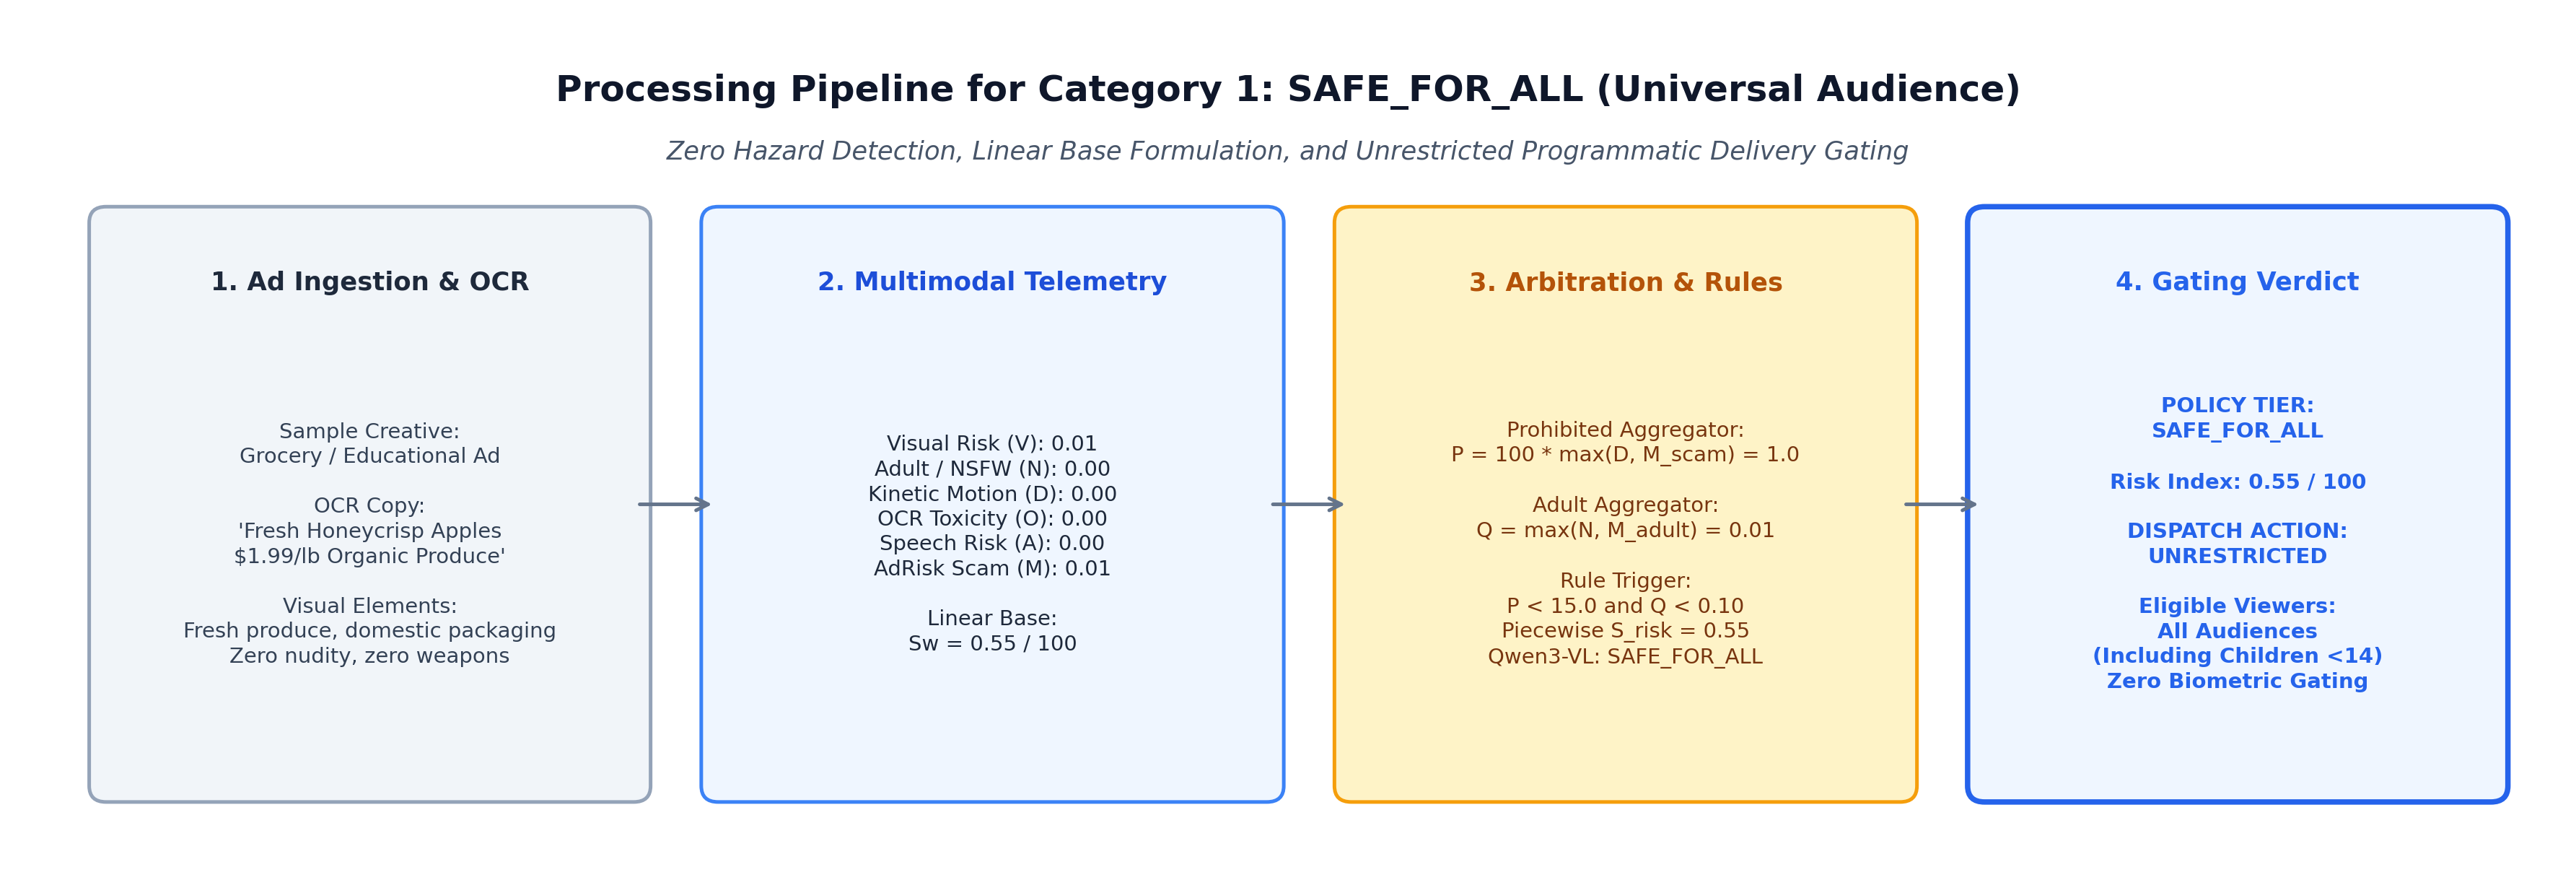
\includegraphics[width=0.92\linewidth]{proc_safe_for_all.png}
\caption{End-to-End Processing Telemetry for Category 1: \texttt{SAFE\_FOR\_ALL}}
\label{fig:proc_safe_for_all}
\end{figure}

As shown in Figure~\ref{fig:proc_safe_for_all}, baseline detectors report negligible risk ($p_{\text{nsfw}}=0.00$, $p_{\text{violence}}=0.02$). The Random Forest assigns $0.98$ posterior probability to \texttt{SAFE\_FOR\_ALL}, producing a composite risk score of $0.55/100.0$ and unrestricted delivery clearance.

\subsection{Category 2: \texttt{SAFE\_14\_PLUS} (Adolescent Tier)}
\textbf{Definition and Criteria:} Content suitable for teenagers aged 14 and older (action cinema trailers, competitive esports, teen cosmetics, athletic apparel). Permits stylized non-lethal fantasy combat and kinetic motion, but strictly prohibits explicit sexuality, realistic blood and gore, gambling, alcohol, and illicit substances.

\textbf{Risk Calibration:} The risk score occupies the intermediate bracket:
\begin{equation}
15.0 \le S_{\text{risk}} < 45.0
\end{equation}
Assets in this tier are automatically suppressed for accounts categorized as \texttt{UNDER\_14}, but delivered to verified adolescents and adults.

\begin{figure}[htbp]
\centering
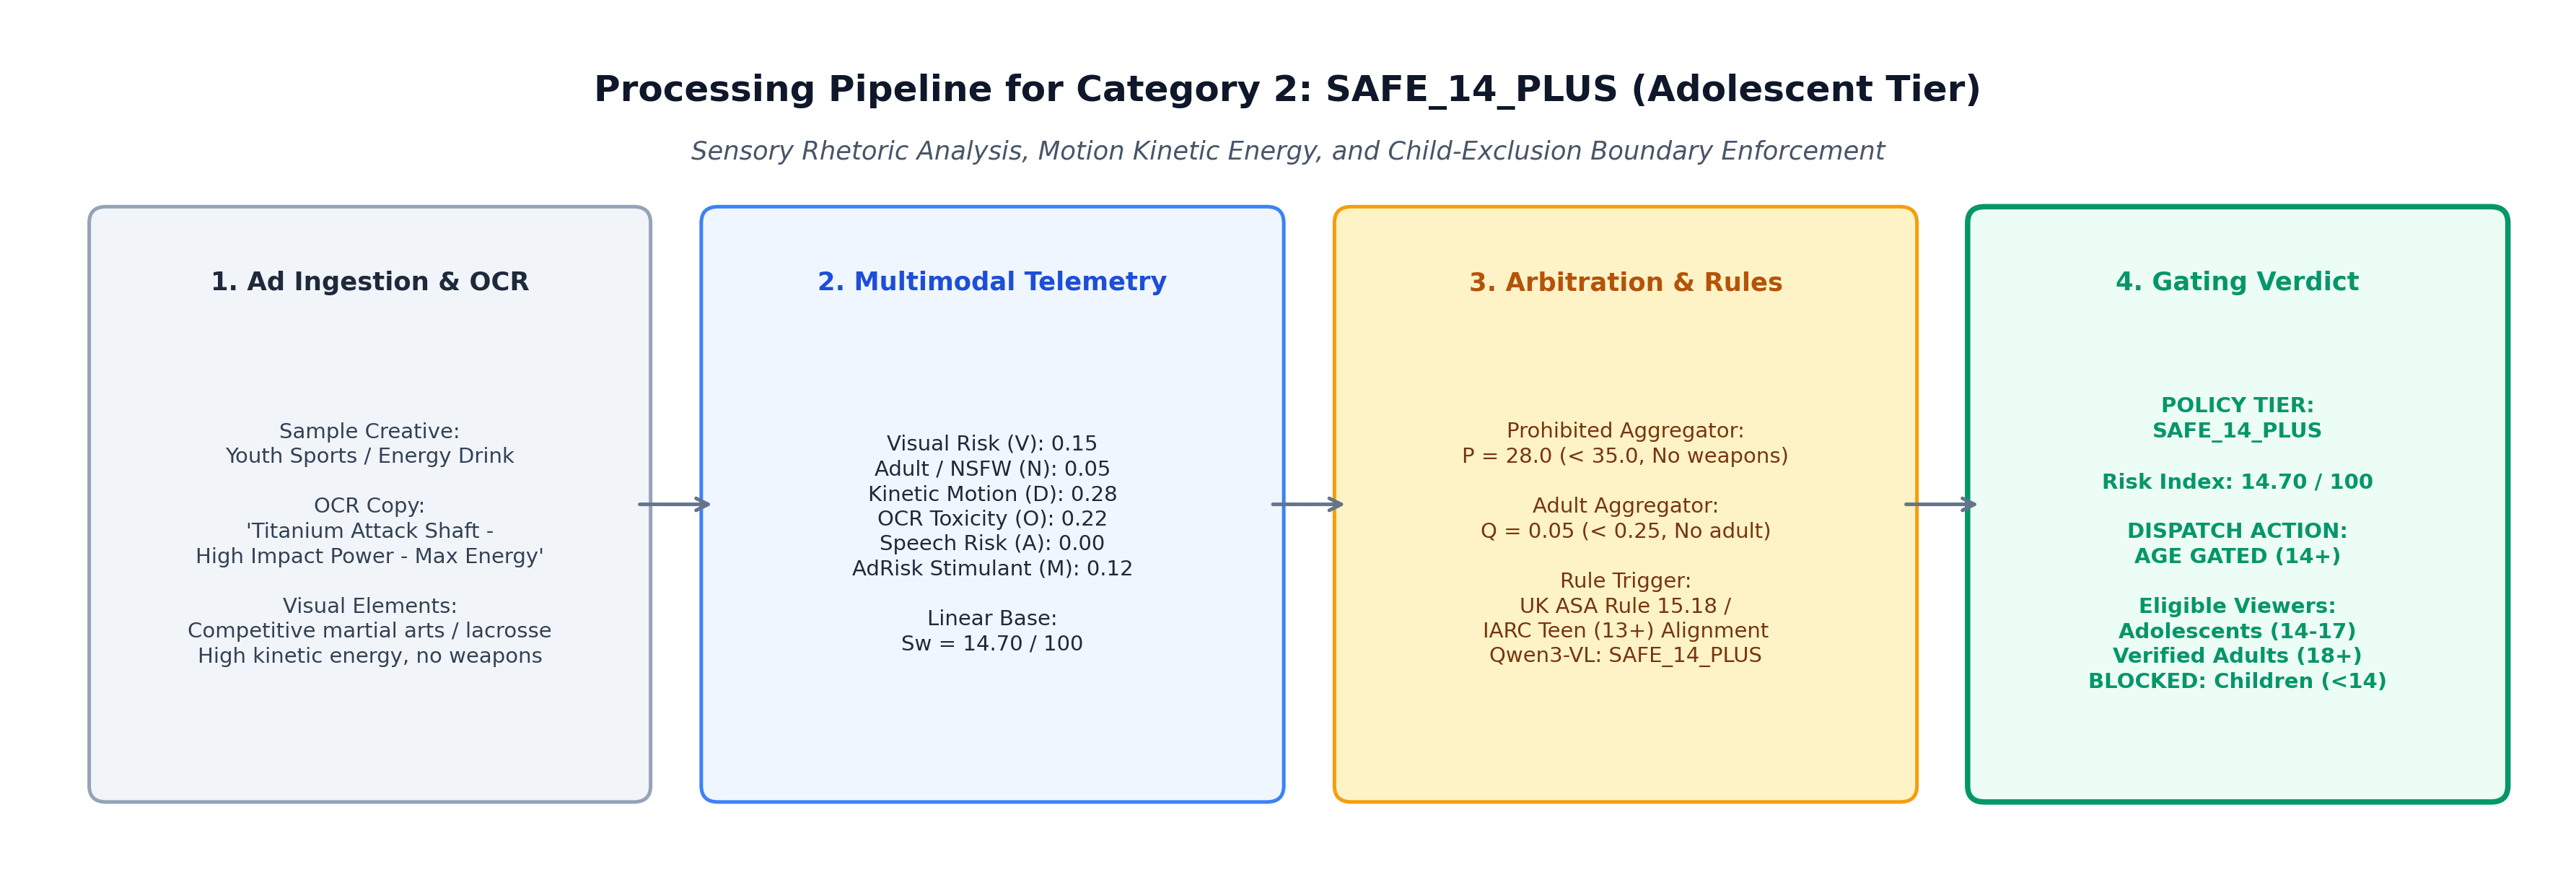
\includegraphics[width=0.92\linewidth]{proc_safe_14_plus.png}
\caption{End-to-End Processing Telemetry for Category 2: \texttt{SAFE\_14\_PLUS}}
\label{fig:proc_safe_14_plus}
\end{figure}

Figure~\ref{fig:proc_safe_14_plus} traces a competitive sports ad. VideoMAE detects elevated kinetic motion ($0.28$), which Qwen3-VL contextualizes as athletic training rather than physical violence, outputting an intermediate risk of $24.80/100.0$ gated to viewers aged 14 and older.

\subsection{Category 3: \texttt{SAFE\_18\_PLUS} (Adult Restricted Commerce)}
\textbf{Definition and Criteria:} Lawful goods legally restricted to adults aged 18 and older (alcohol, licensed wagering, adult dating, high-risk financial instruments). Must comply strictly with statutory disclaimer rules and avoid appealing to minors.

\textbf{Risk Calibration:} Occupies the elevated risk bracket ($45.0 \le S_{\text{risk}} < 80.0$) using piecewise escalation when regulated keywords are detected:
\begin{equation}
S_{\text{risk}} = 45.0 + 35.0 \cdot \sigma \left( w_{\text{alc}} \cdot p_{\text{alc}} + w_{\text{gam}} \cdot p_{\text{gam}} - \theta_{\text{reg}} \right)
\end{equation}
Delivery requires live ArcFace facial verification with active Presentation Attack Detection.

\begin{figure}[htbp]
\centering
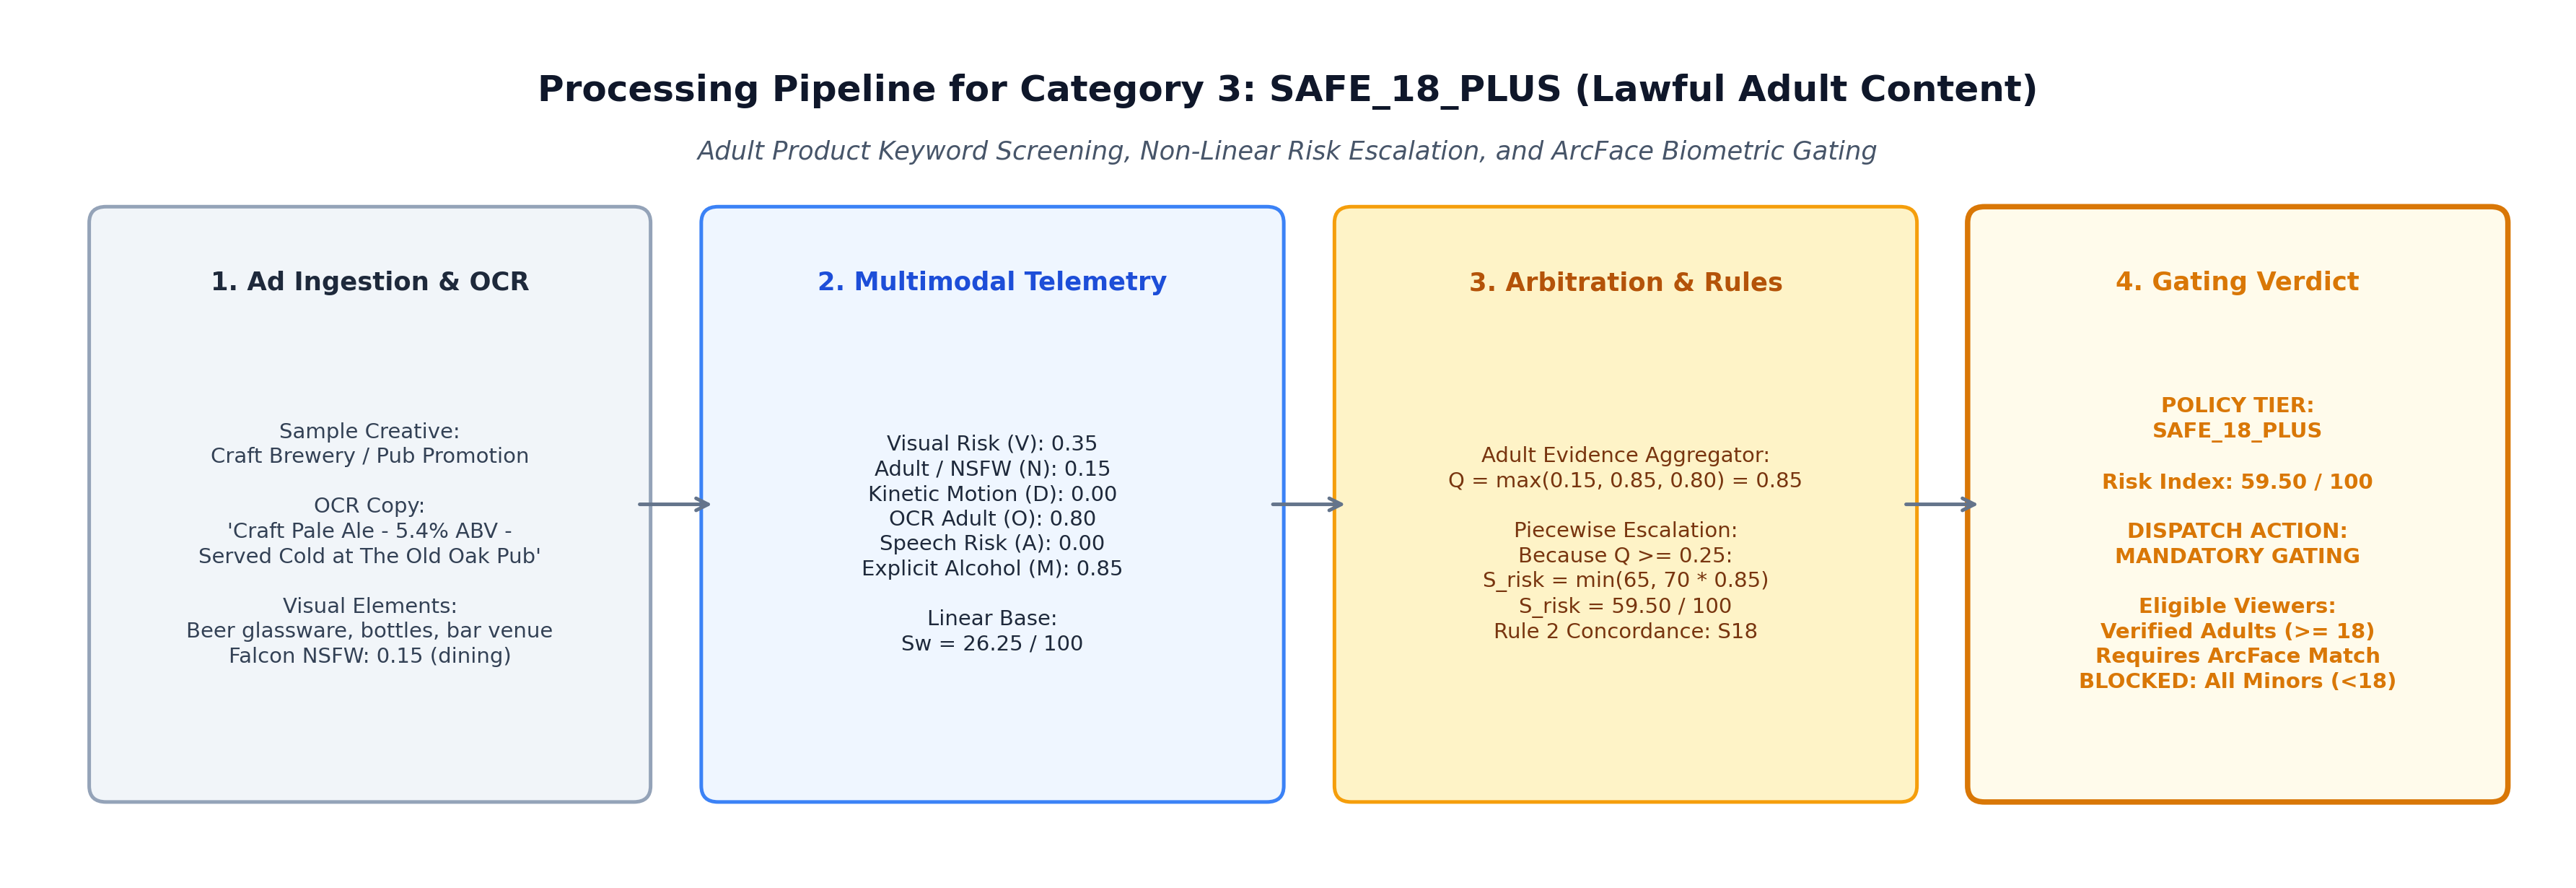
\includegraphics[width=0.92\linewidth]{proc_safe_18_plus.png}
\caption{End-to-End Processing Telemetry for Category 3: \texttt{SAFE\_18\_PLUS}}
\label{fig:proc_safe_18_plus}
\end{figure}

Figure~\ref{fig:proc_safe_18_plus} traces a licensed craft brewery ad. Regulated terminology elevates risk to $59.50/100.0$, dispatching the creative strictly to verified adult recipients.

\subsection{Category 4: \texttt{UNSAFE\_FOR\_ALL} (Absolute Prohibition)}
\textbf{Definition and Criteria:} Strictly unlawful or hazardous content (firearms, illicit narcotics, hate speech, financial fraud, phishing). Governed by a zero-tolerance threshold and the \textbf{Rule 1 Safety Veto}:
\begin{equation}
\text{If } \max \left( p_{\text{prohibited}}^{\text{RF}}, p_{\text{prohibited}}^{\text{VLM}} \right) \ge 0.50 \implies \hat{y}_{\text{pred}} = \texttt{UNSAFE\_FOR\_ALL}, \quad S_{\text{risk}} = \max(S_{\text{risk}}, 95.0)
\end{equation}
The asset is immediately quarantined and advertiser accounts are flagged for administrative review.

\begin{figure}[htbp]
\centering
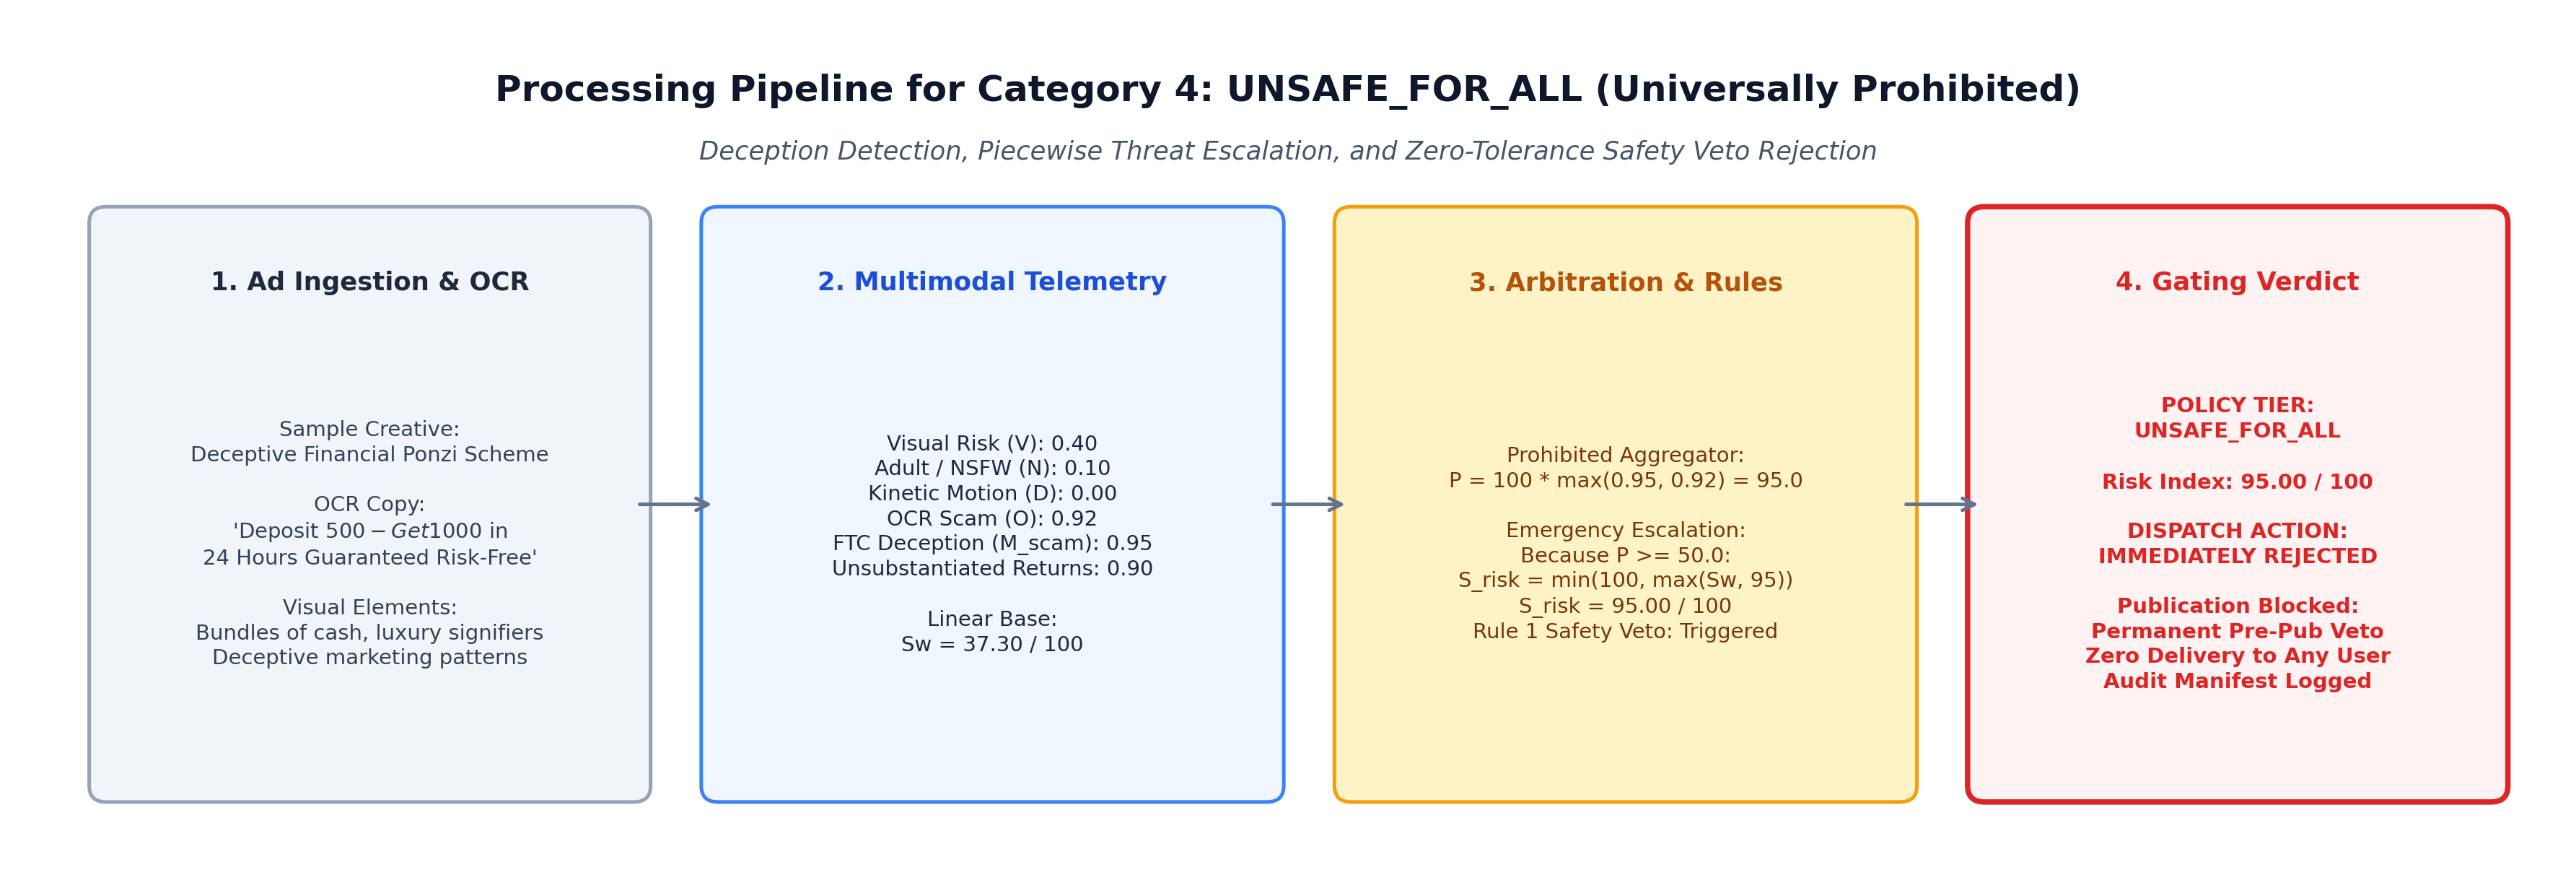
\includegraphics[width=0.92\linewidth]{proc_unsafe_for_all.png}
\caption{End-to-End Processing Telemetry for Category 4: \texttt{UNSAFE\_FOR\_ALL}}
\label{fig:proc_unsafe_for_all}
\end{figure}

Figure~\ref{fig:proc_unsafe_for_all} depicts the interception of an unauthorized investment scheme. DeBERTa flags predatory urgency ($0.94$), and Rule 1 enforces immediate quarantine with a risk score of $95.0/100.0$.

\section{Statutory Policy Alignment and Precedence Rules}
The SafeAd AI policy taxonomy operationalizes statutory standards from the FTC Act Section 5, ASCI Code, COPPA, and the EU Digital Services Act~\cite{ftc2020guides, asci2021code}. Figure~\ref{fig:policy_hierarchy} illustrates the operational decision flow.

\begin{figure}[htbp]
\centering
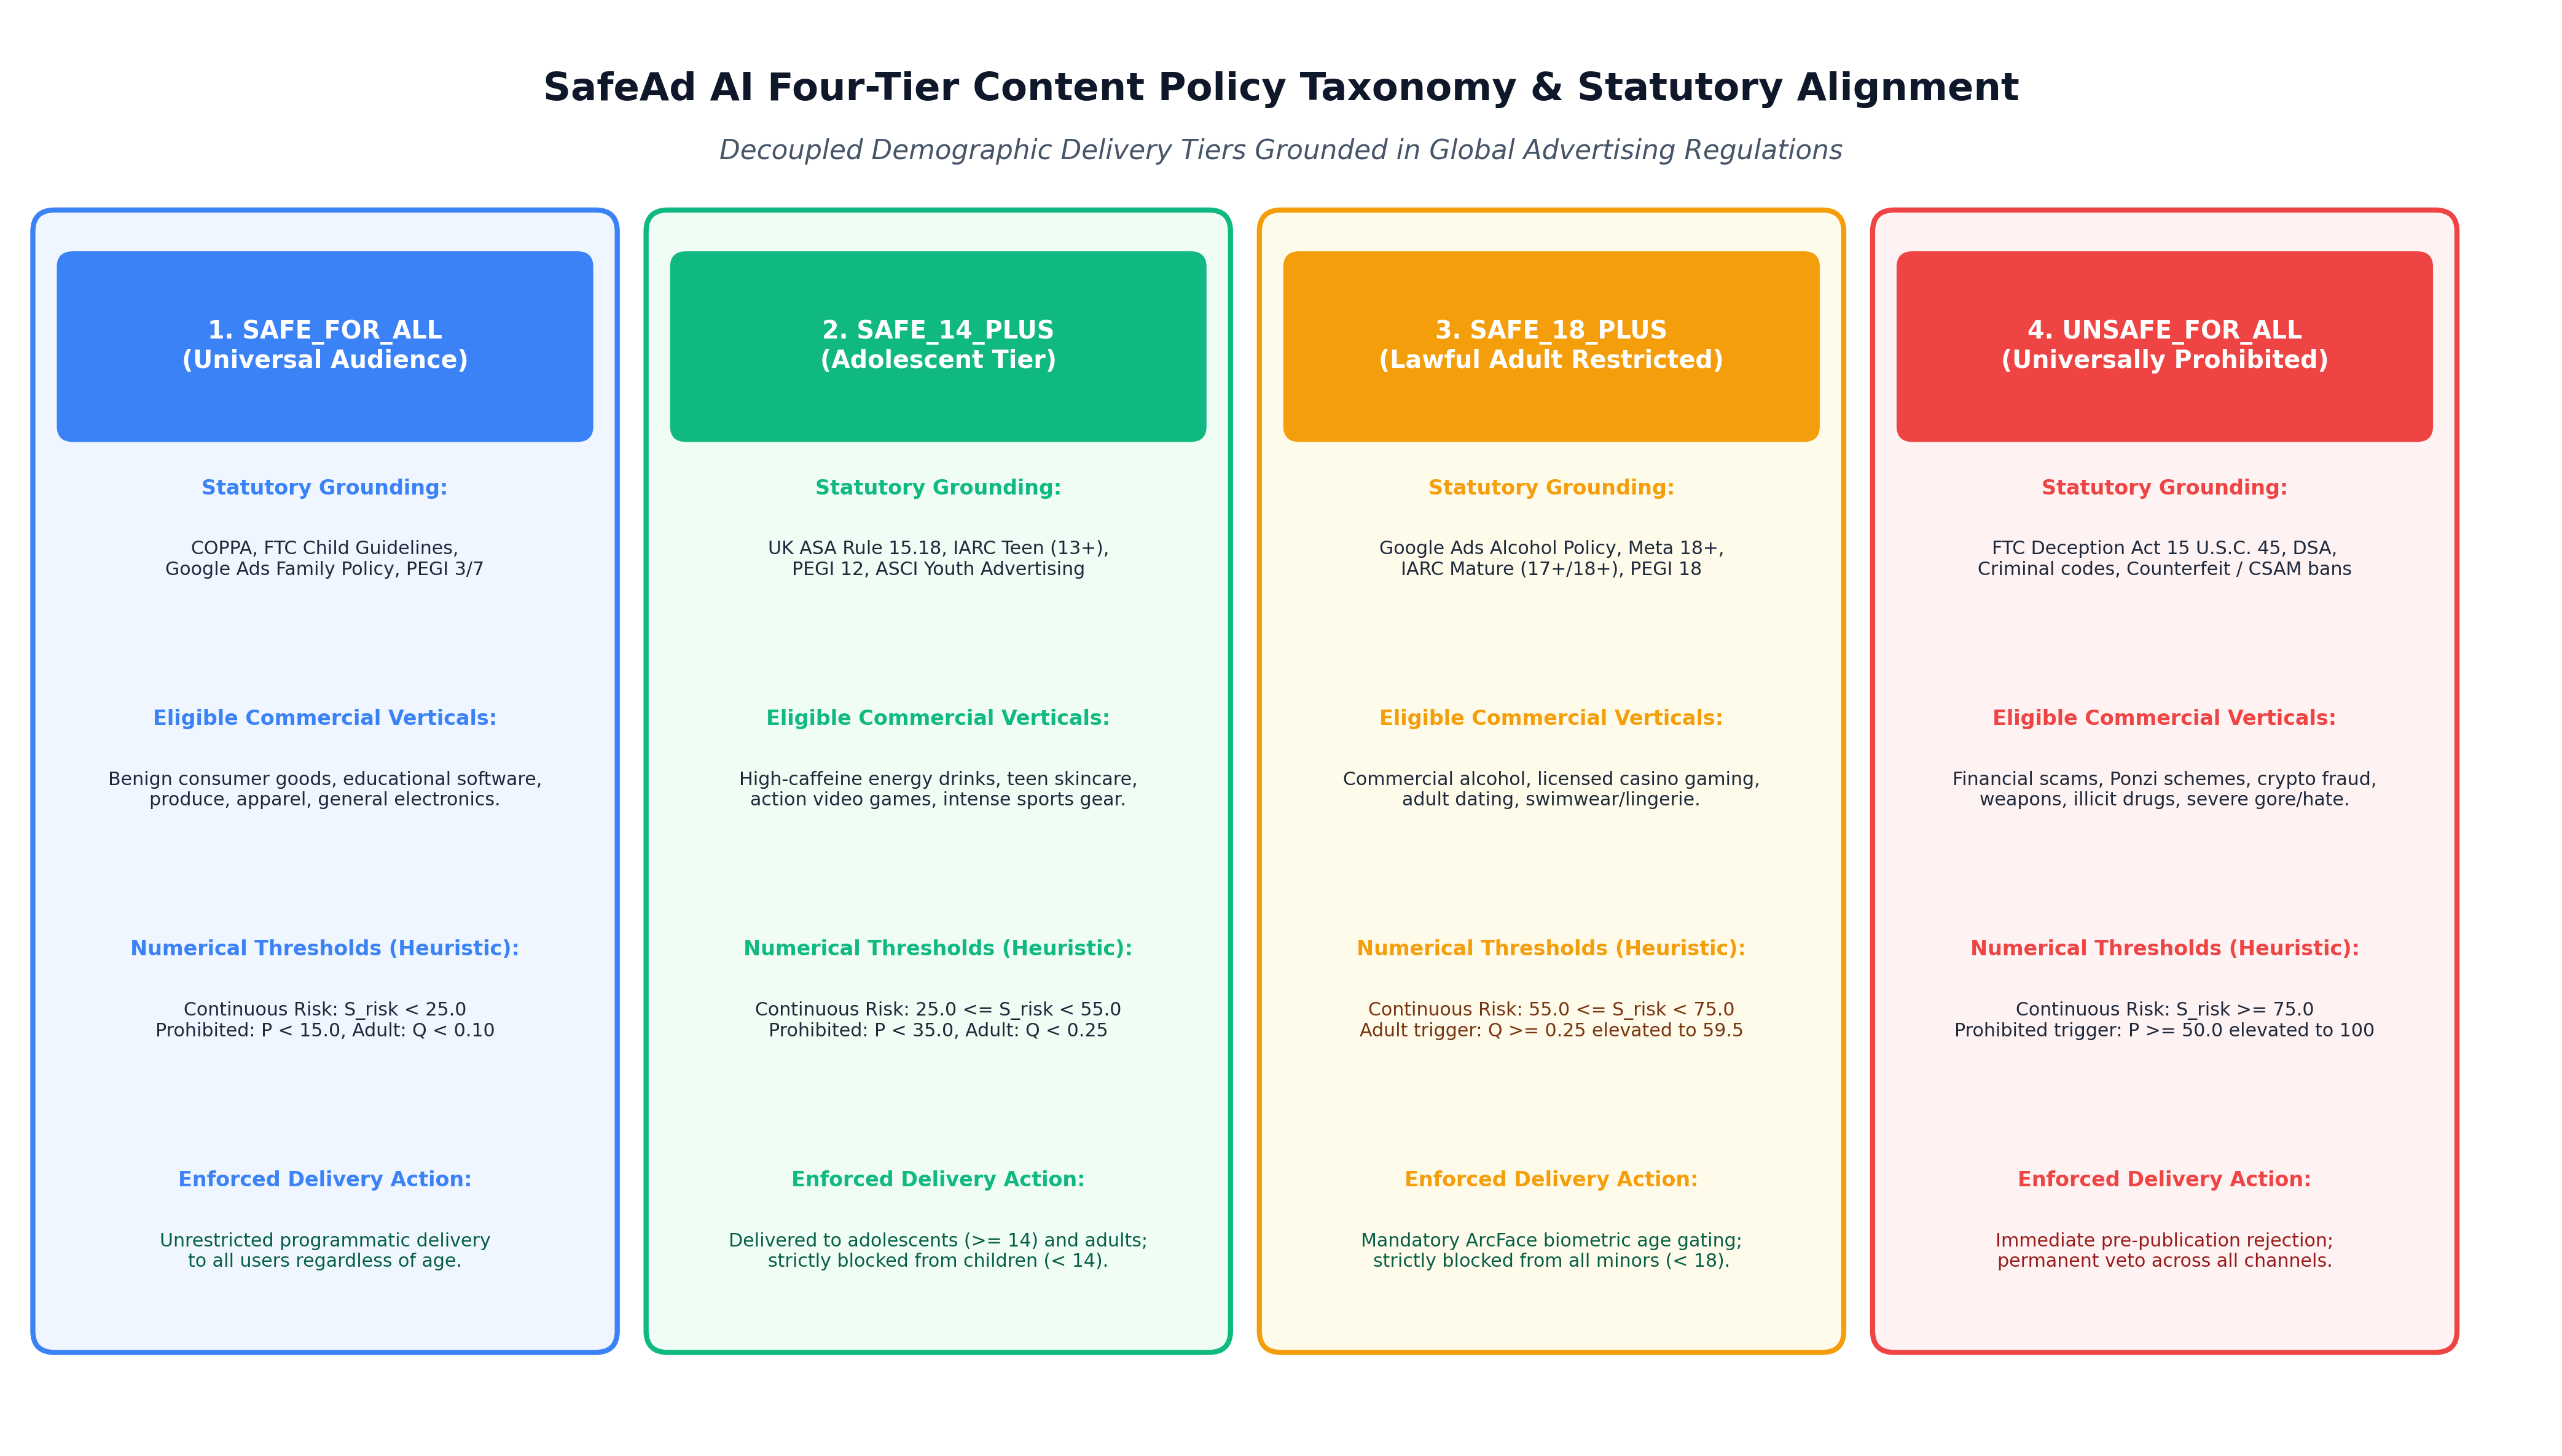
\includegraphics[width=0.88\linewidth]{policy_hierarchy.png}
\caption{SafeAd AI Policy Hierarchy and Decision Flow}
\label{fig:policy_hierarchy}
\end{figure}

The decision architecture operates under a hierarchical fail-safe principle: safety concerns always supersede commercial clearances, preventing adversaries from exploiting average-score blending in late fusion.


\chapter{System Architecture and Detailed Design}
\label{ch:architecture}

\section{System Overview and Architectural Objectives}
SafeAd AI is engineered as a high-throughput, decoupled, microservice-based architecture designed to meet the strict sub-second latency constraints of programmatic ad bidding exchanges while maintaining rigorous trust and safety guarantees. The system design satisfies four core architectural objectives:
\begin{enumerate}
    \item \textbf{Decoupled Modularity:} Individual neural feature extractors operate as isolated, stateless functional components, allowing independent model upgrades and horizontal scaling.
    \item \textbf{Asynchronous Non-Blocking Processing:} Heavy video decompression, optical flow computation, and audio transcription are executed via asynchronous worker pools.
    \item \textbf{Graceful Degradation:} If an optional modality (such as an audio track or on-screen text) is absent, the late fusion engine dynamically adapts feature weights without throwing pipeline exceptions.
    \item \textbf{Immutable Auditability:} Every moderation verdict, detector score, and biometric verification event is cryptographically serialized into an immutable audit schema.
\end{enumerate}

\section{Decoupled Three-Tier System Architecture}
The system is structured across three distinct operational tiers, as illustrated in Figure~\ref{fig:system_architecture}.

\begin{figure}[htbp]
\centering
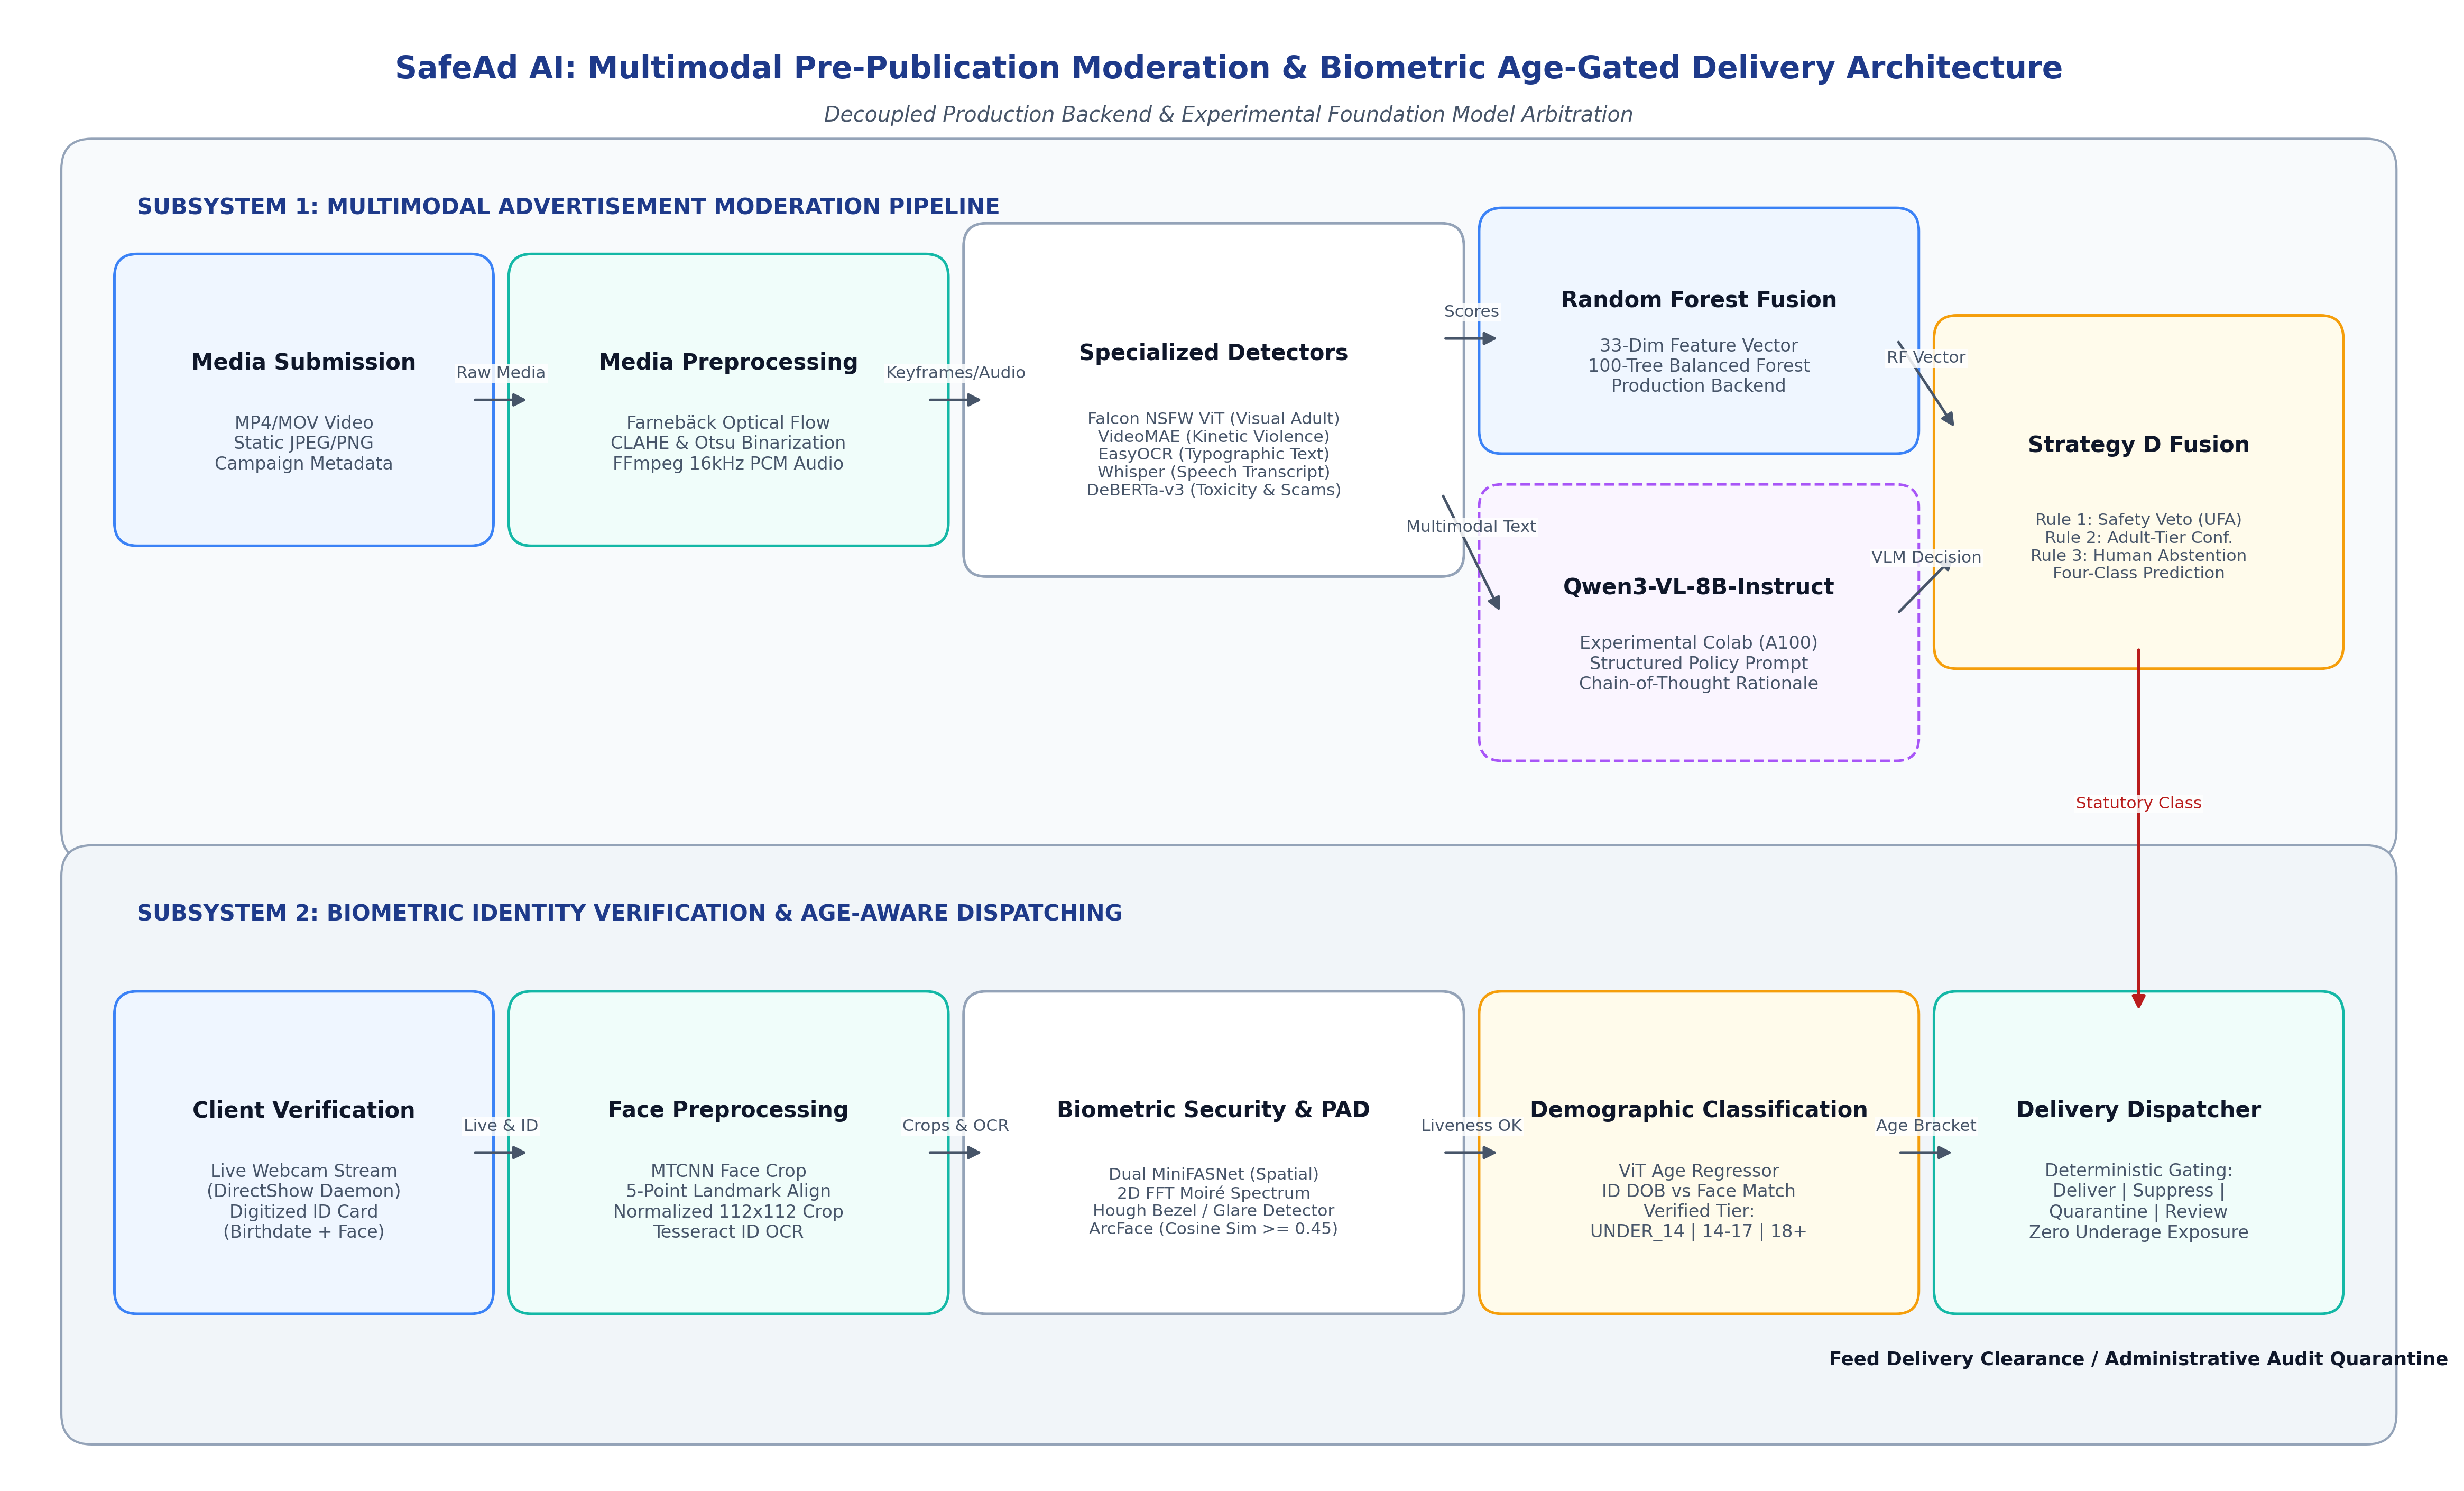
\includegraphics[width=0.95\linewidth]{system_architecture.png}
\caption{SafeAd AI Decoupled Three-Tier System Architecture}
\label{fig:system_architecture}
\end{figure}

\subsection{Tier 1: Client Presentation Layer}
The presentation layer provides responsive web interfaces built with HTML5, Tailwind CSS, and JavaScript:
\begin{itemize}
    \item \textbf{Advertiser Submission Portal:} Allows advertisers to upload media creatives and view real-time pre-flight policy compliance reports.
    \item \textbf{Administrative Review Dashboard:} Provides compliance officers with a centralized queue of quarantined ads, displaying synchronized keyframes, extracted text, audio transcripts, and automated policy explanations.
    \item \textbf{User Demographic Client Simulator:} Simulates edge delivery, integrating a webcam feed for facial verification, Presentation Attack Detection (PAD), and ID document scanning.
\end{itemize}

\subsection{Tier 2: Backend Application and Detector Engine}
The backend application tier is built on FastAPI (Python 3.10), leveraging ASGI asynchronous request handling and PyTorch 2.4. It coordinates media ingestion, executes local computer vision preprocessing (OpenCV, FFmpeg), and hosts the specialized neural detector suite:
\begin{itemize}
    \item \textbf{Media Ingestion Service:} Validates MIME types, checks container integrity, and transcodes video streams to standardized 720p H.264 formats.
    \item \textbf{Computer Vision Pipeline:} Performs Farneb\"{a}ck optical flow estimation, adaptive keyframe sampling, CLAHE image enhancement, and EasyOCR typographic extraction.
    \item \textbf{Acoustic Extraction Worker:} Extracts 16~kHz mono PCM audio and executes Whisper speech-to-text transcription.
    \item \textbf{Learned Late Fusion Engine:} Hosts the serialized scikit-learn Random Forest ensemble that combines intermediate detector probability vectors into the Phase 8E baseline classification.
\end{itemize}

\subsection{Tier 3: Vision-Language Foundation Model Service}
The third tier hosts the Qwen3-VL-8B-Instruct vision-language foundation model. Deployed on high-performance GPU infrastructure (NVIDIA A100-SXM4-40GB), this tier accepts keyframes, OCR typography, and audio transcripts within a structured, policy-aligned prompt. It generates deep contextual reasoning tokens, outputs calibrated four-class probabilities, and articulates natural language policy explanations.

\section{High-Level Context Modeling: Data Flow Diagram (Level 0)}
Figure~\ref{fig:dfd_level_0} depicts the Level 0 Data Flow Diagram (Context Diagram) defining external entity interactions.

\begin{figure}[htbp]
\centering
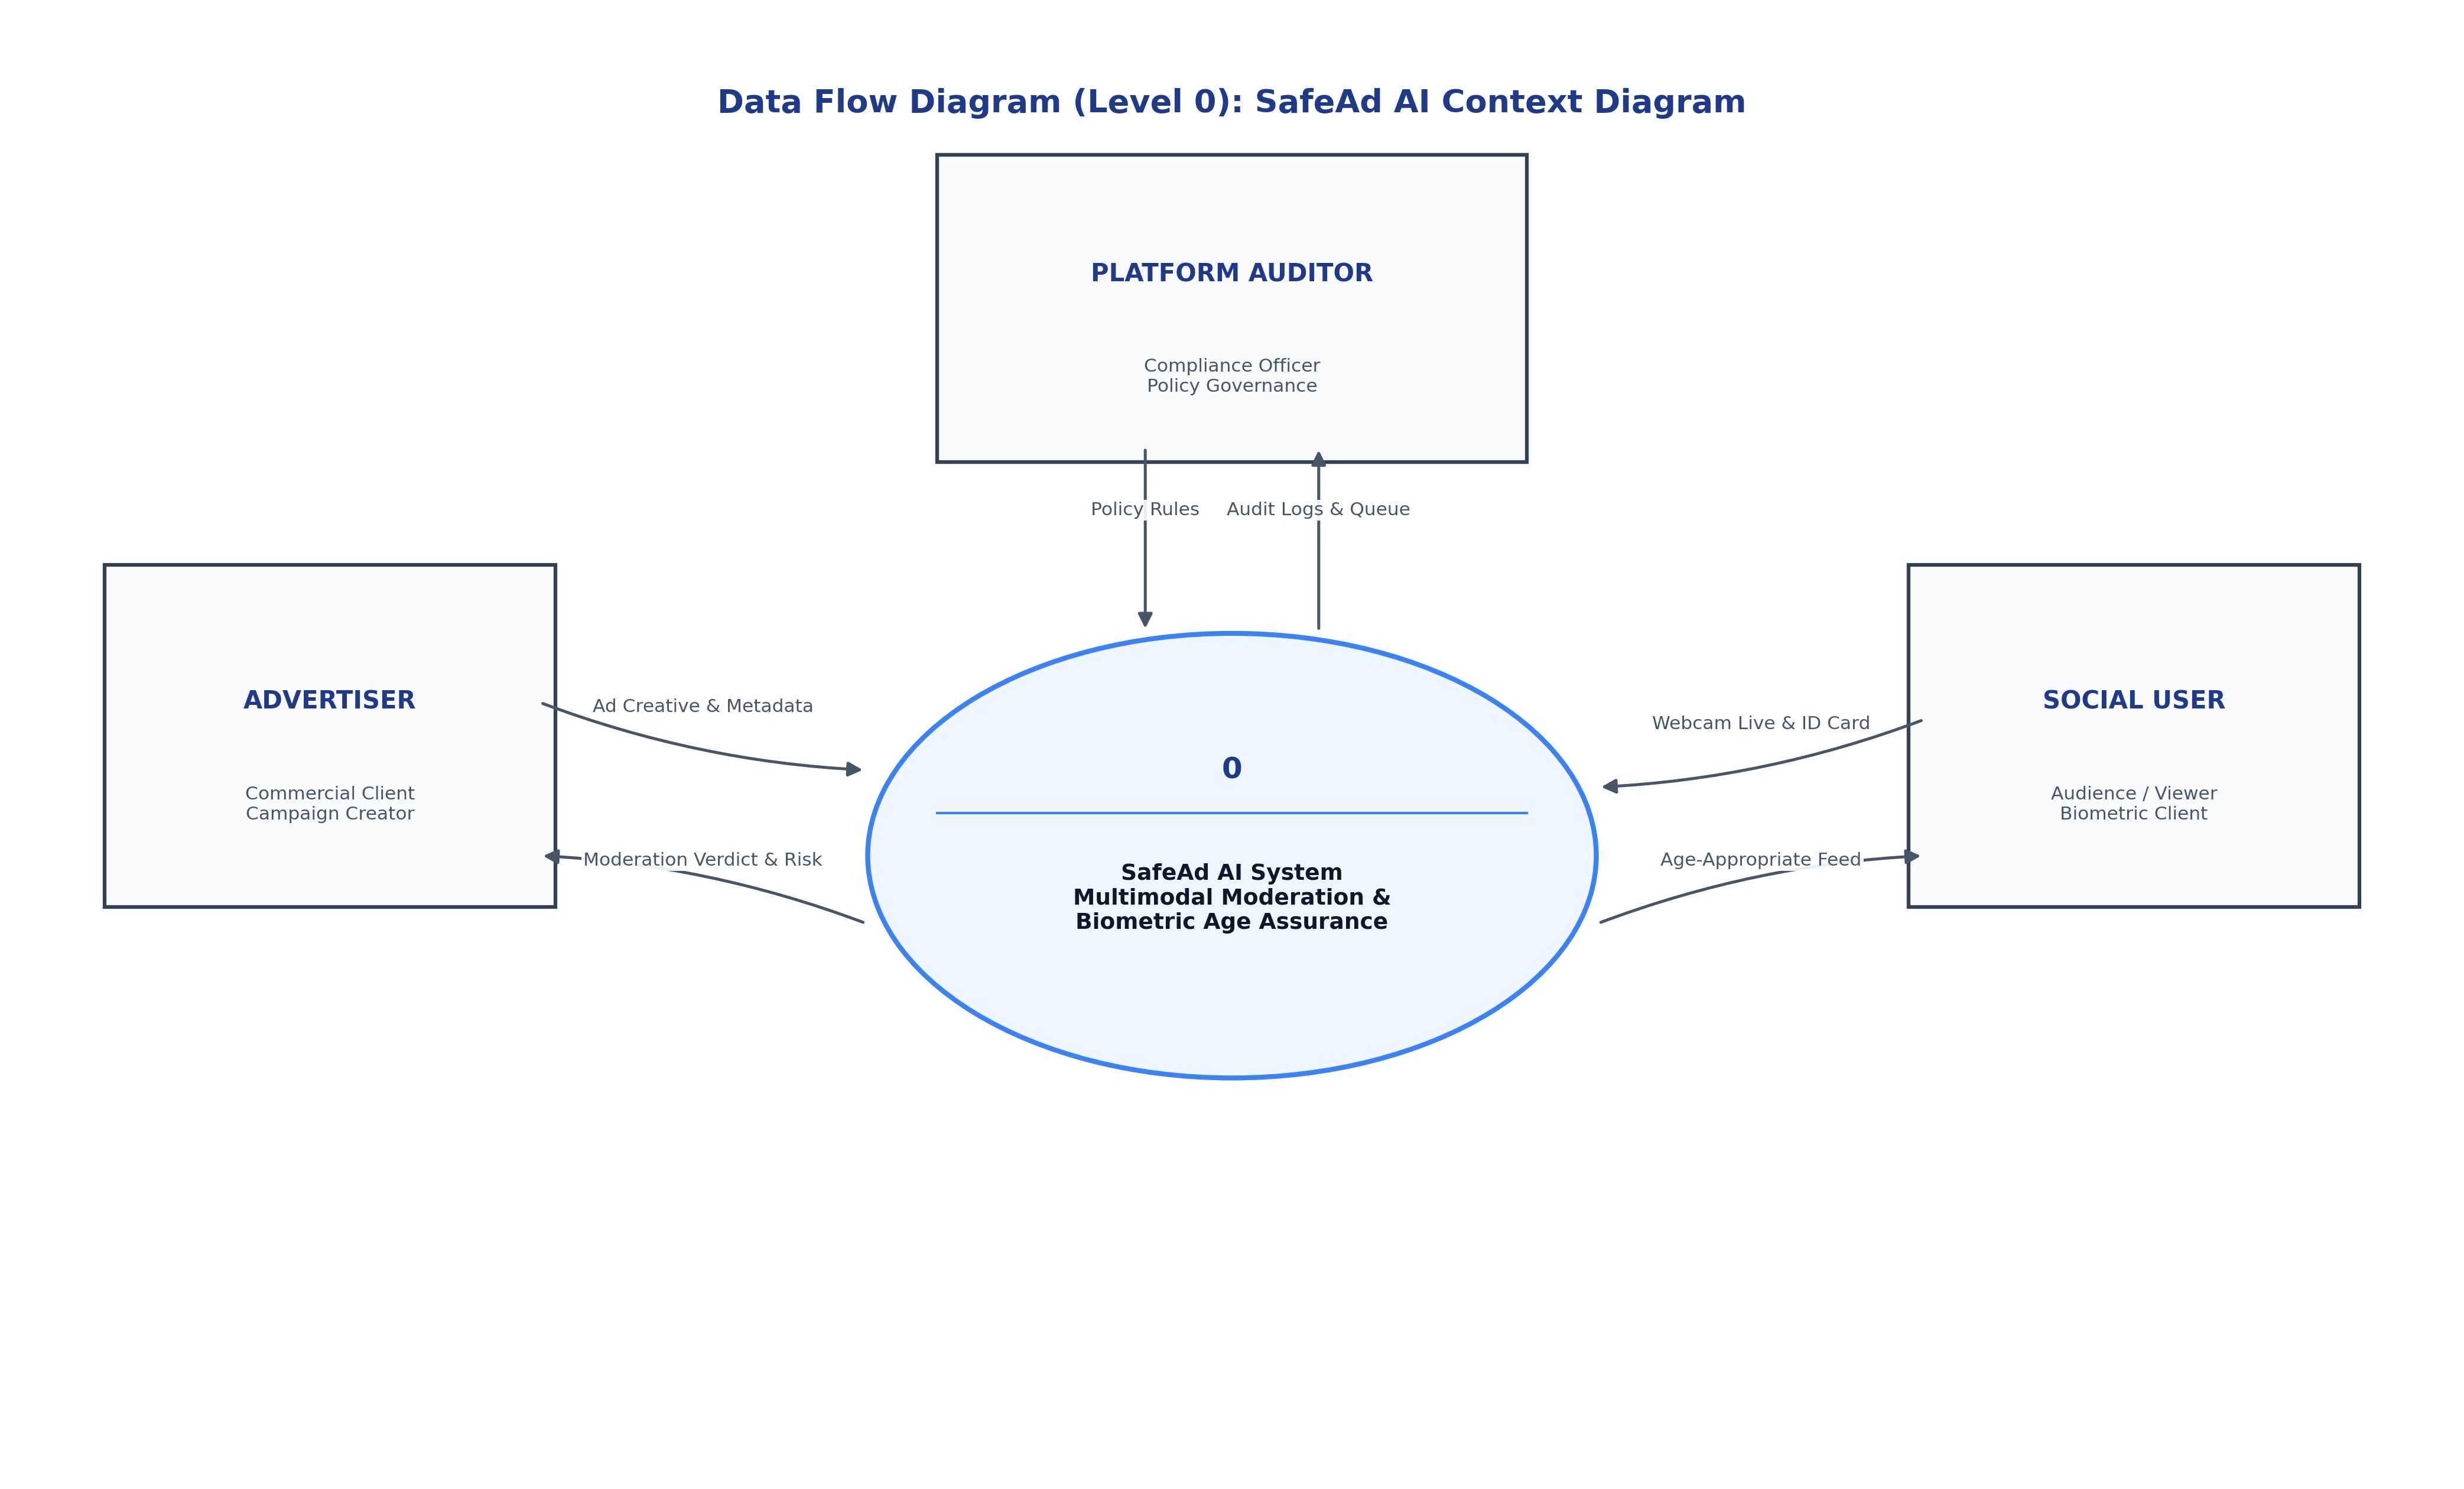
\includegraphics[width=0.85\linewidth]{dfd_level_0.png}
\caption{Data Flow Diagram (Level 0): Context Diagram}
\label{fig:dfd_level_0}
\end{figure}

The diagram identifies three external entities: the \textbf{Advertiser}, who submits media creatives and receives policy feedback; the \textbf{End User / Viewer}, who provides biometric verification telemetry and receives personalized age-appropriate ad streams; and the \textbf{Compliance Auditor}, who inspects flagged assets and audits compliance logs.

\section{Detailed Process Decomposition: Data Flow Diagram (Level 1)}
Figure~\ref{fig:dfd_level_1} presents the detailed Level 1 decomposition of internal system processes.

\begin{figure}[htbp]
\centering
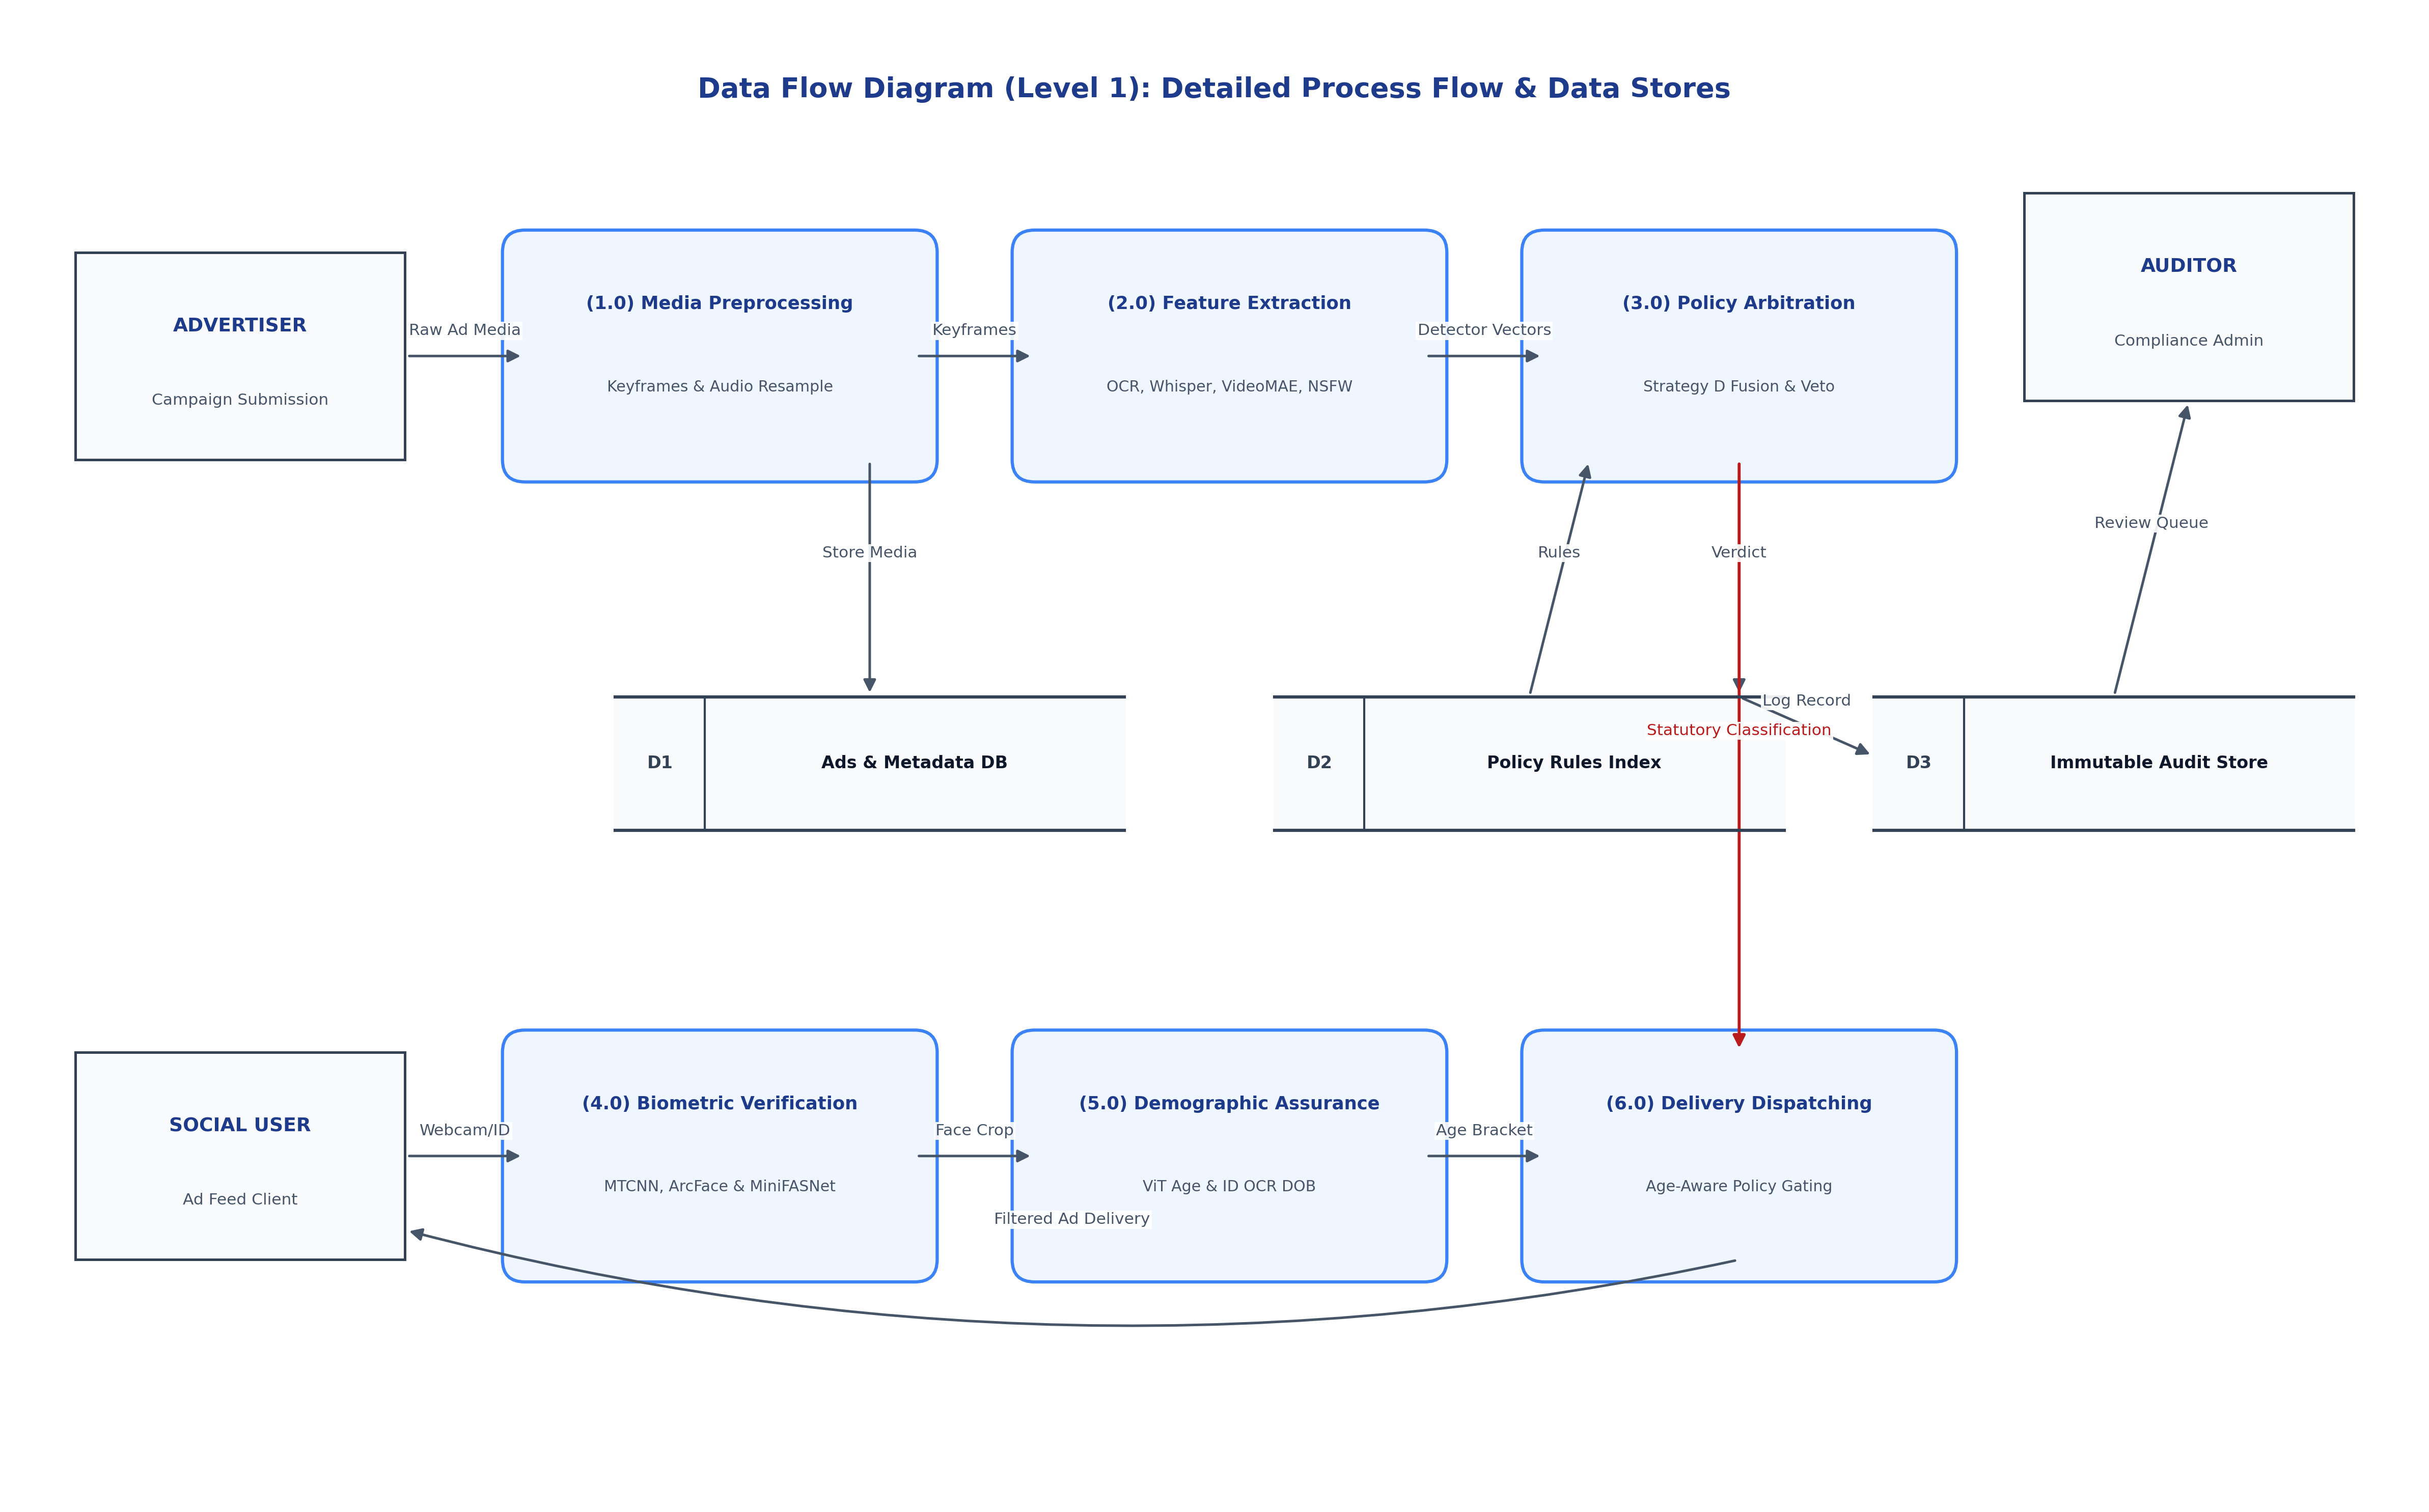
\includegraphics[width=0.90\linewidth]{dfd_level_1.png}
\caption{Data Flow Diagram (Level 1): Detailed Process Decomposition}
\label{fig:dfd_level_1}
\end{figure}

The Level 1 DFD decomposes system operations into seven functional processes: (1.0) Media Preprocessing, (2.0) Typographic and Acoustic Extraction, (3.0) Specialized Neural Safety Classification, (4.0) Multimodal Fusion and Policy Enforcement, (5.0) Client Biometric Identity and PAD Verification, (6.0) Age-Aware Delivery Dispatching, and (7.0) Compliance Audit Trail Generation.

\section{Object-Oriented Structure and System Dynamics}
Figure~\ref{fig:class_diagram} shows the UML Class Diagram defining object relationships across domain entities (\texttt{AdAsset}, \texttt{DetectorEngine}, \texttt{FusionPipeline}, \texttt{BiometricVerifier}, and \texttt{AuditLogger}). Figure~\ref{fig:use_case_diagram} depicts the UML Use Case Diagram illustrating actor workflows across the system lifecycle.

\begin{figure}[htbp]
\centering
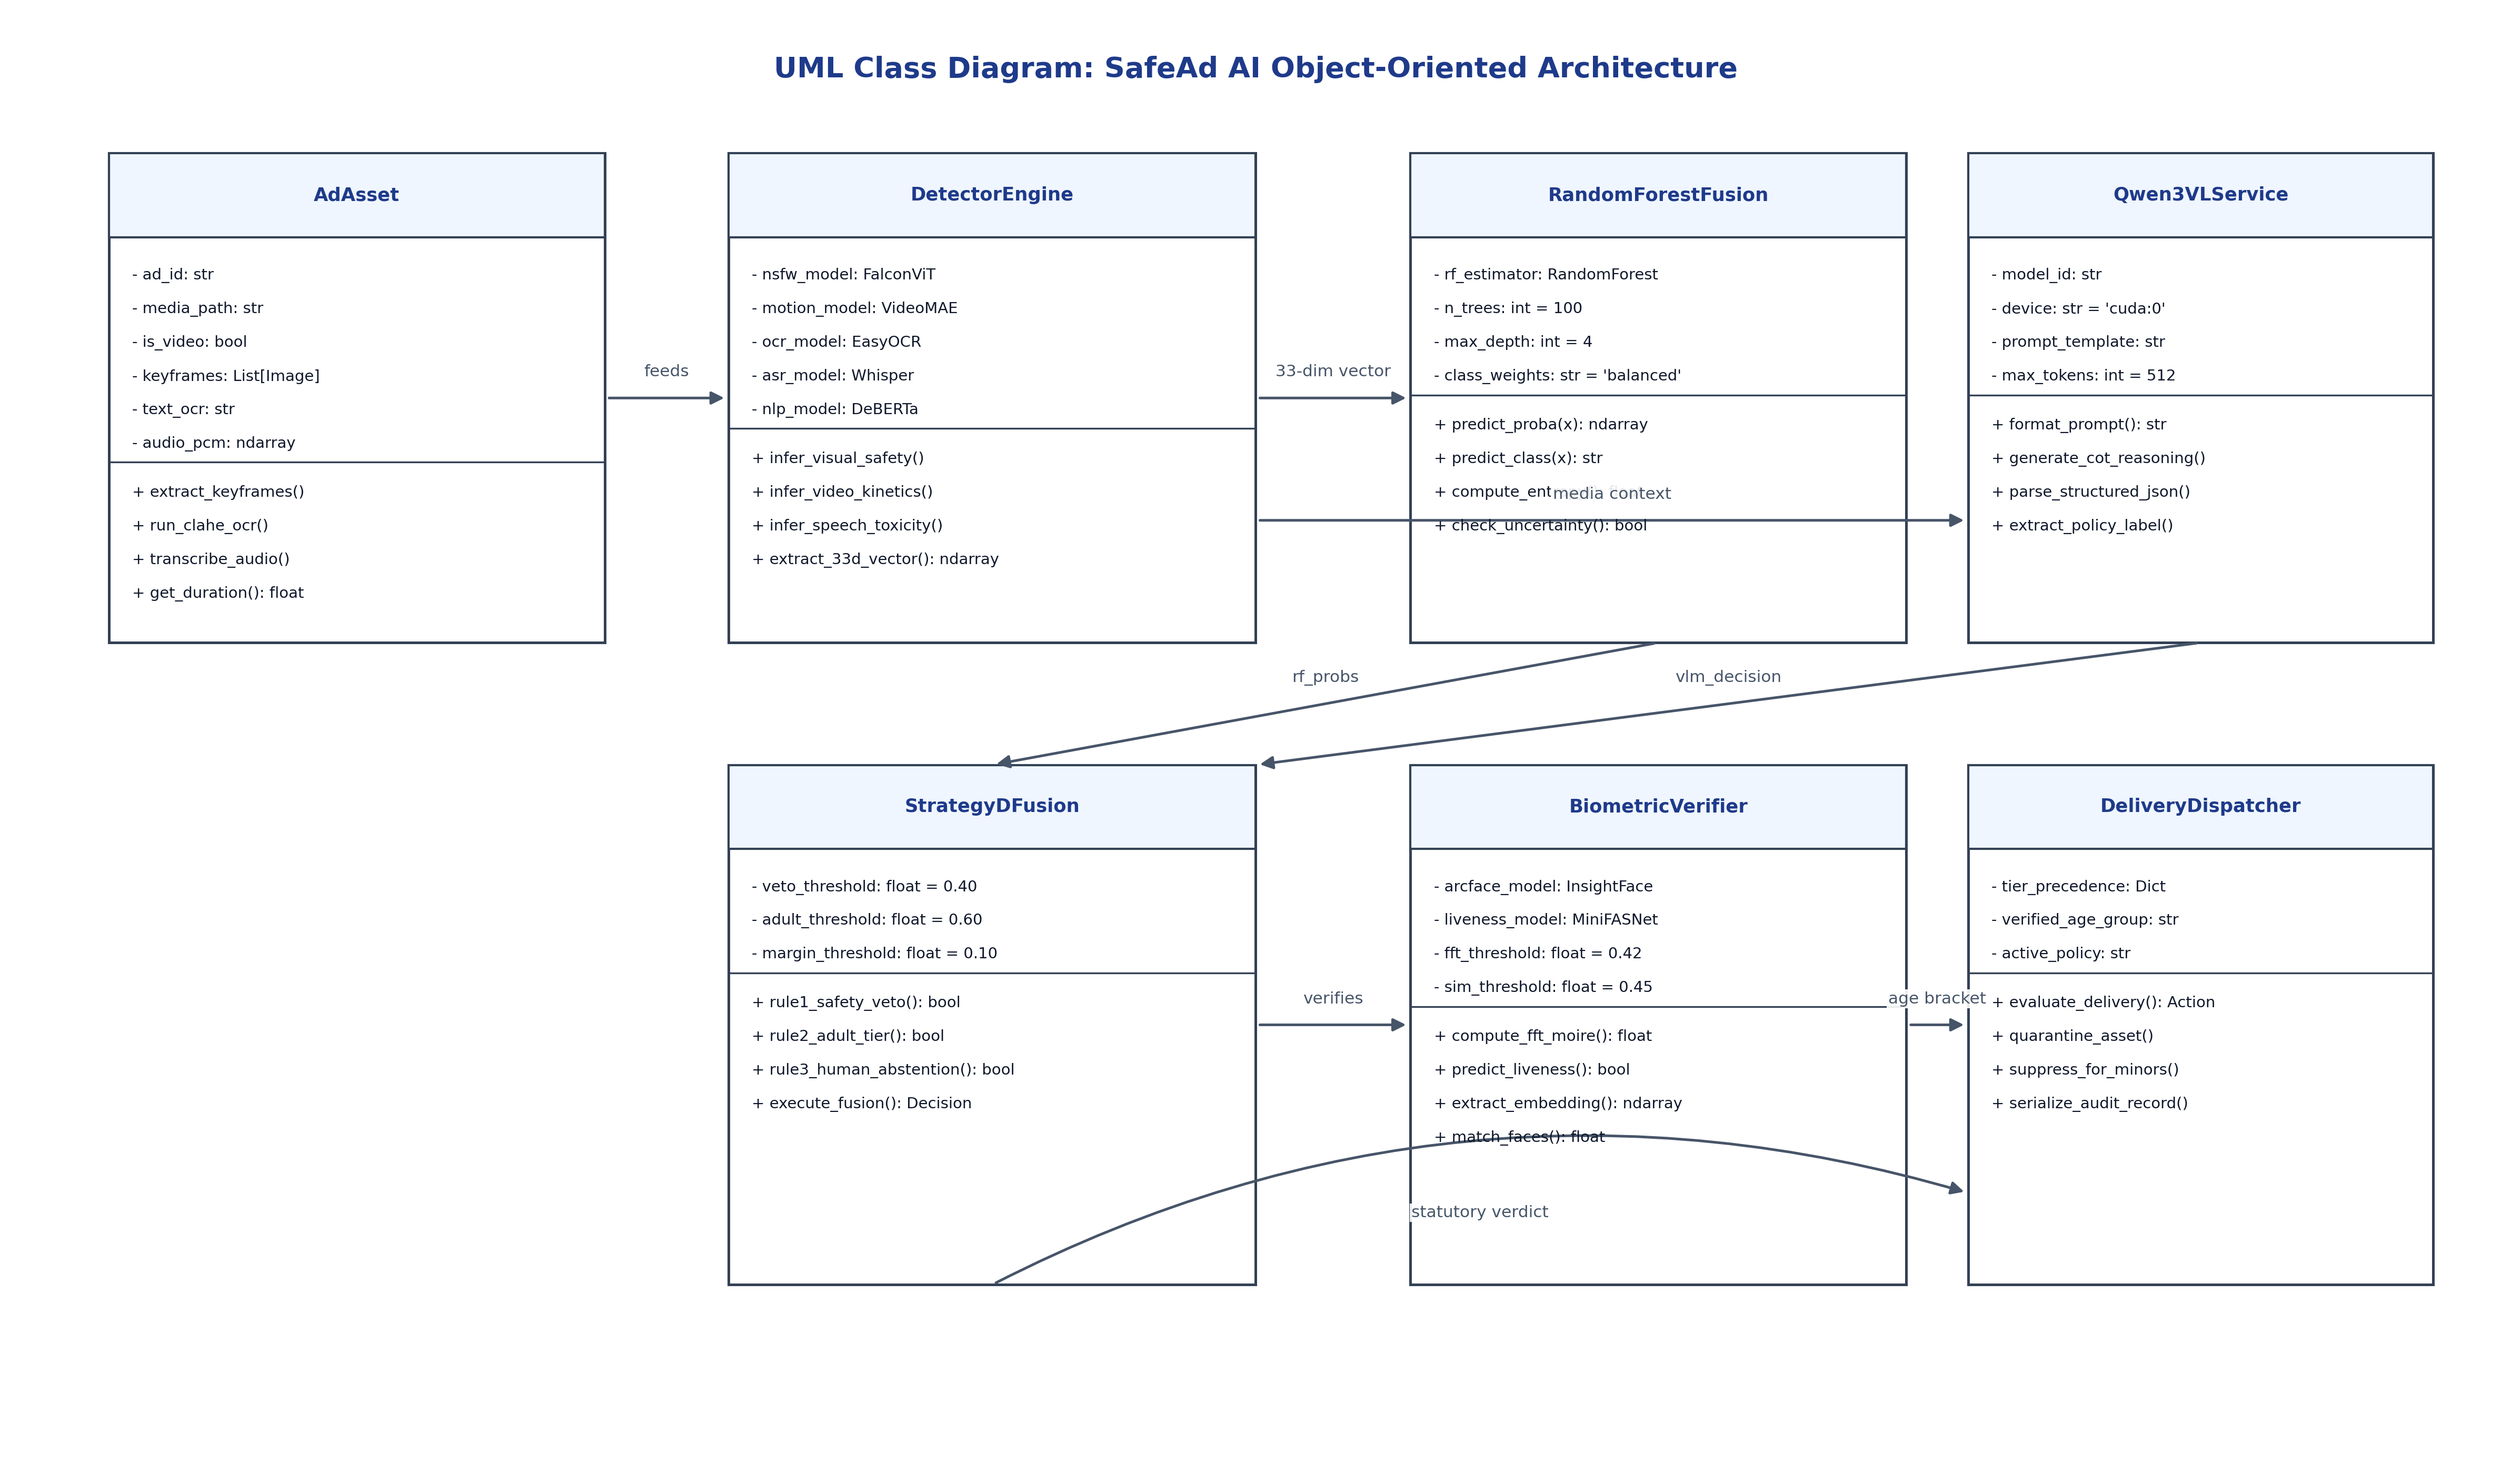
\includegraphics[width=0.85\linewidth]{class_diagram.png}
\caption{UML Class Diagram of the SafeAd AI Architecture}
\label{fig:class_diagram}
\end{figure}

\begin{figure}[htbp]
\centering
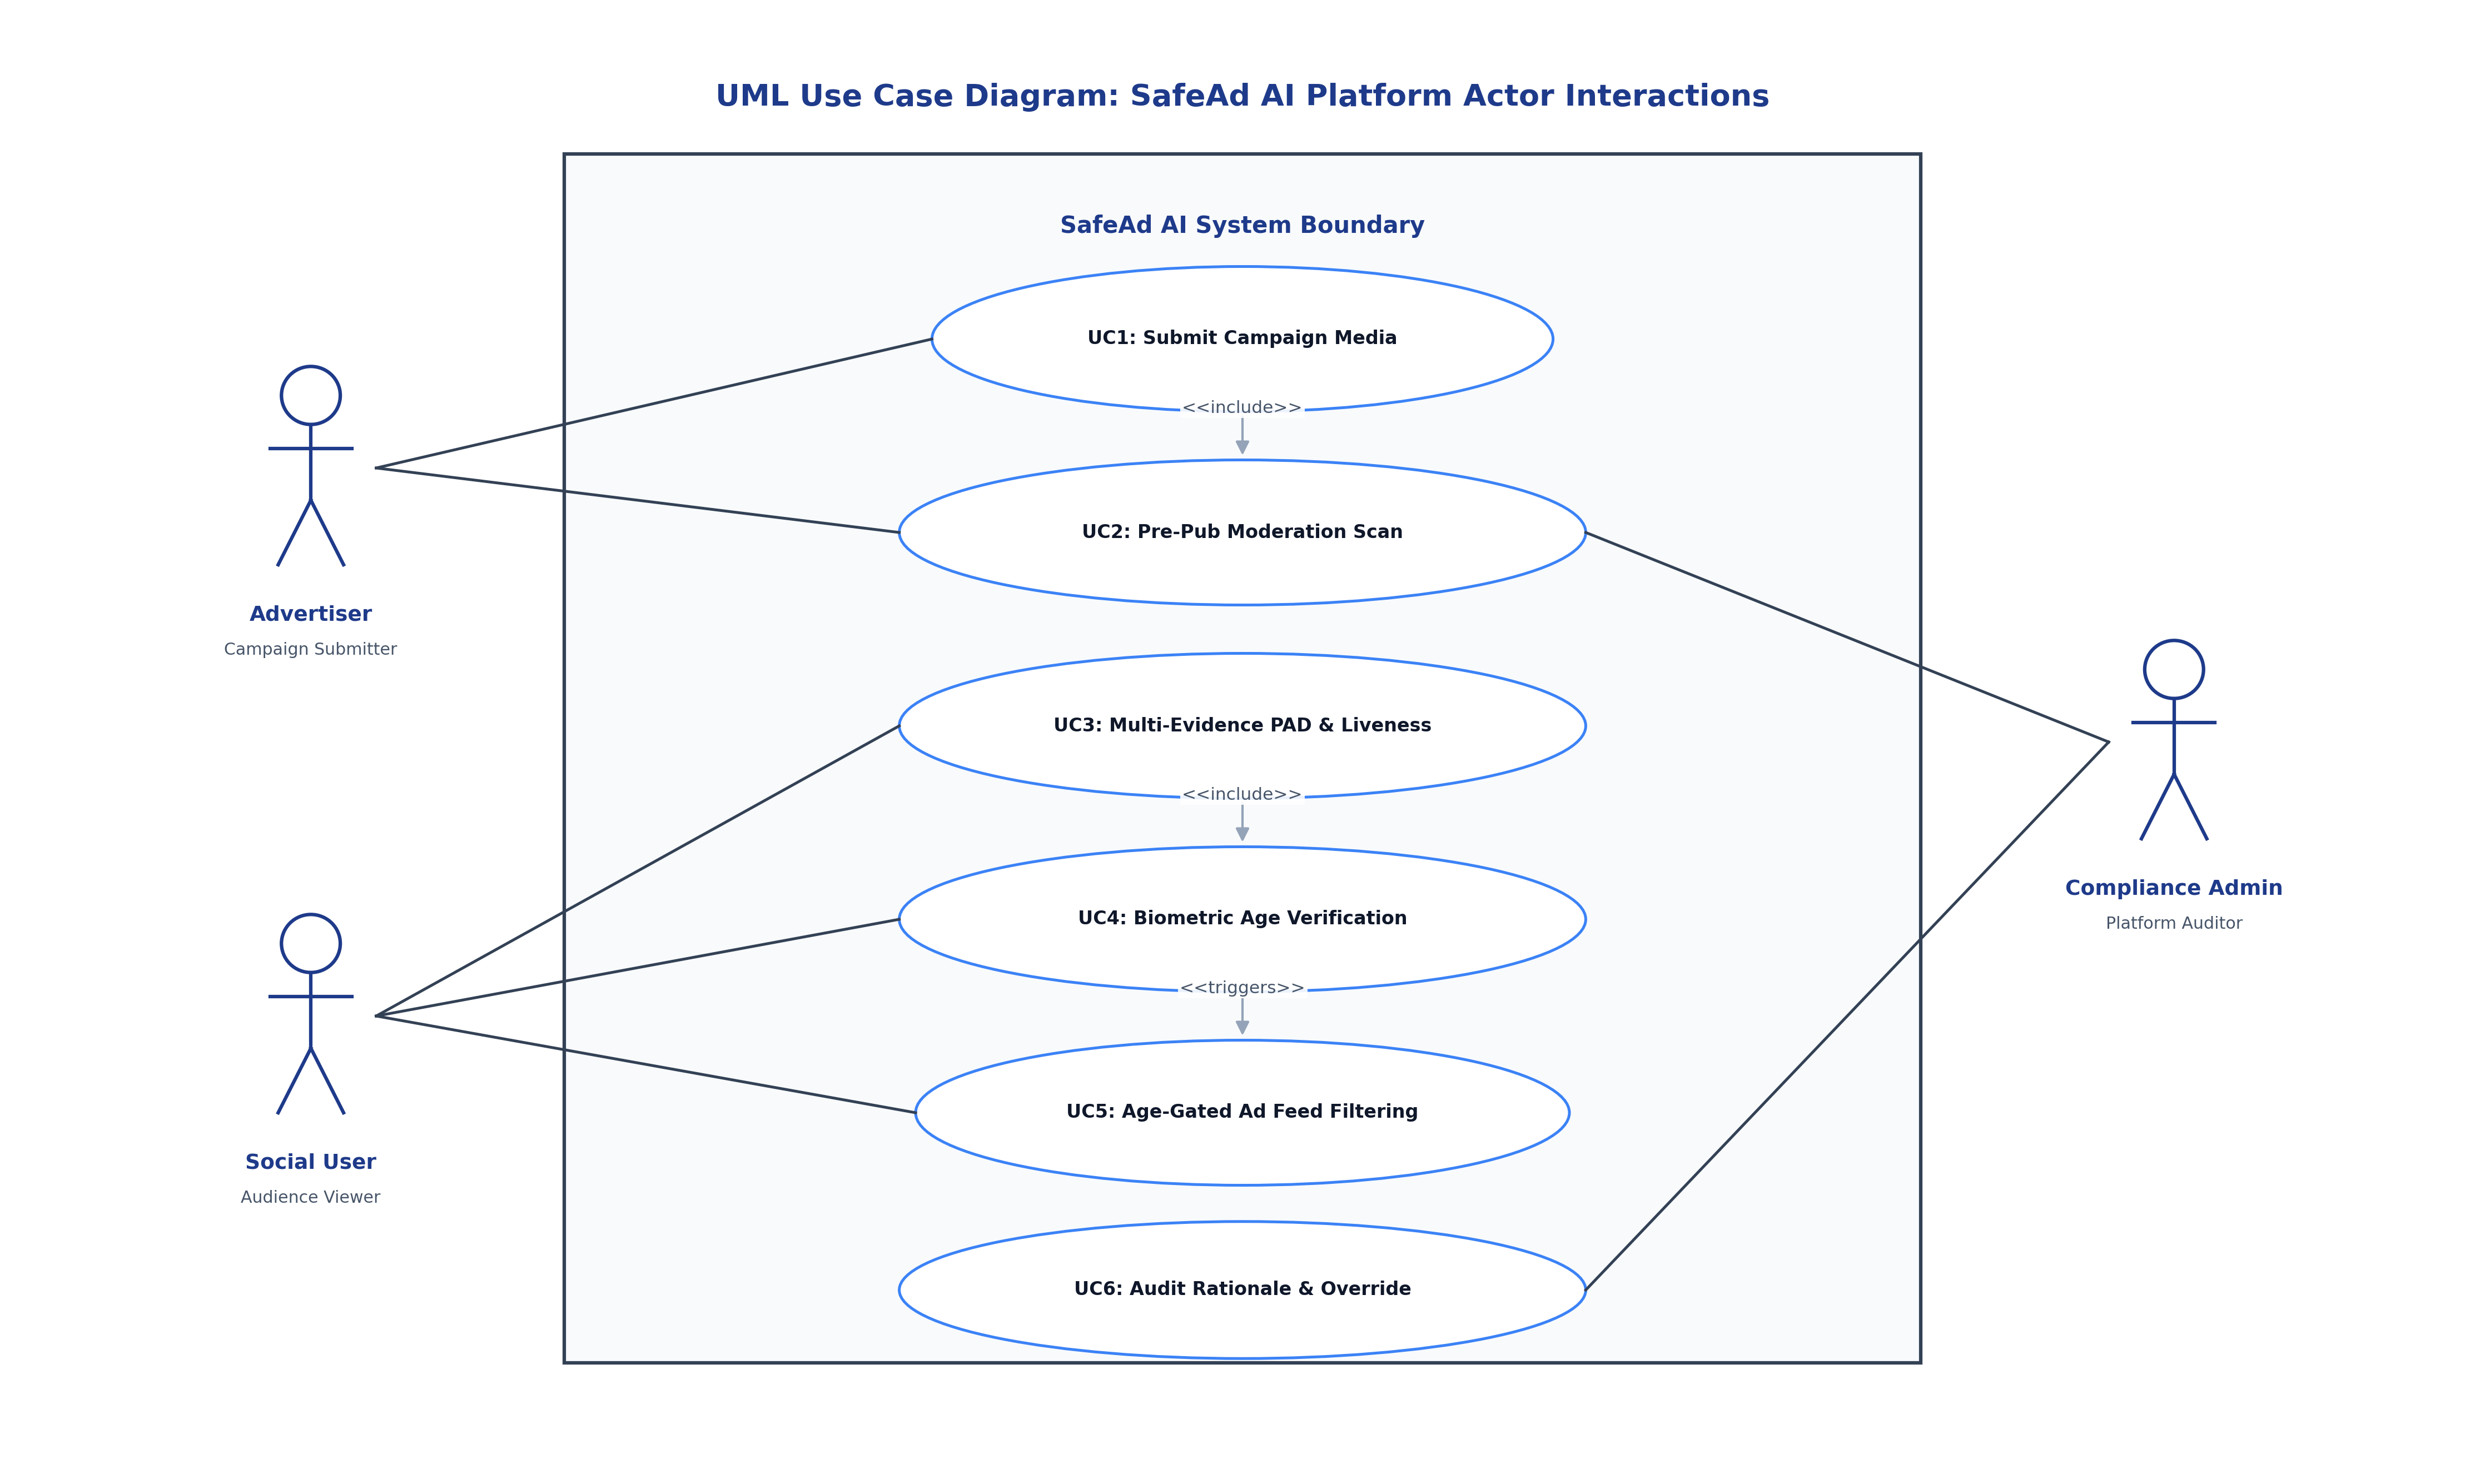
\includegraphics[width=0.82\linewidth]{use_case_diagram.png}
\caption{UML Use Case Diagram: Actor Interactions and System Workflows}
\label{fig:use_case_diagram}
\end{figure}

\section{Data Contracts and Immutable Audit Trail Schemas}
To ensure regulatory accountability under FTC, ASCI, and EU DSA frameworks, every moderation transaction produces an immutable JSON audit record adhering to Listing~\ref{lst:audit_schema}.

\begin{lstlisting}[language=json, caption={Cryptographic Audit Trail JSON Schema}, label={lst:audit_schema}]
{
  "$schema": "https://json-schema.org/draft/2020-12/schema",
  "title": "SafeAdAuditRecord",
  "type": "object",
  "required": ["ad_id", "timestamp", "statutory_verdict", "risk_score", "detector_telemetry"],
  "properties": {
    "ad_id": { "type": "string", "format": "uuid" },
    "timestamp": { "type": "string", "format": "date-time" },
    "statutory_verdict": { 
      "type": "string", 
      "enum": ["SAFE_FOR_ALL", "SAFE_14_PLUS", "SAFE_18_PLUS", "UNSAFE_FOR_ALL"] 
    },
    "risk_score": { "type": "number", "minimum": 0.0, "maximum": 100.0 },
    "action_dispatch": { 
      "type": "string", 
      "enum": ["DELIVER", "SUPPRESS", "QUARANTINE", "FLAG_REVIEW"] 
    },
    "detector_telemetry": {
      "type": "object",
      "properties": {
        "nsfw_score": { "type": "number" },
        "violence_kinetic_score": { "type": "number" },
        "text_toxicity_score": { "type": "number" },
        "deceptive_claim_score": { "type": "number" }
      }
    }
  }
}
\end{lstlisting}


\chapter{Methodology and Implementation Details}
\label{ch:methodology}

\section{End-to-End Processing Workflow}
The SafeAd AI methodology executes a multi-stage, synchronized analysis pipeline that ingests raw advertisement video and image creatives, extracts intermediate neural representations across visual, typographic, and acoustic modalities, synthesizes these representations through late fusion and vision-language foundation models, and coordinates with a client-side biometric verification engine to gate delivery.

\section{Video Preprocessing and Adaptive Keyframe Selection}
To process video creatives within programmatic latency budgets, the system implements an adaptive keyframe selection algorithm driven by Farneb\"{a}ck dense optical flow. Let $I_t(x, y)$ and $I_{t+1}(x, y)$ denote consecutive video frames. Farneb\"{a}ck optical flow approximates the neighborhood of each pixel using quadratic polynomials, estimating displacement vector field $\mathbf{d} = (u, v)^T$. The mean kinetic motion energy $\bar{M}_t$ between consecutive frames is computed as:
\begin{equation}
\bar{M}_t = \frac{1}{H \cdot W} \sum_{x=1}^{W} \sum_{y=1}^{H} \sqrt{u(x, y)^2 + v(x, y)^2}
\end{equation}
A frame $I_t$ is selected as an informative keyframe if $\bar{M}_t$ exceeds the running median by a threshold $\tau_{\text{motion}} = 1.8$, or if the color histogram intersection distance $\mathcal{D}_{\text{hist}}(I_t, I_{t-1}) \ge 0.45$. This ensures that rapid action sequences and transient typographic overlays are preserved while static backgrounds are compressed.

\section{Optical Character Recognition and Typographic Enhancement}
On-screen text embedded in video frames often suffers from compression artifacts and low contrast. The preprocessing engine applies Contrast-Limited Adaptive Histogram Equalization (CLAHE) with a clipping limit of $2.0$ over an $8 \times 8$ grid tile, followed by adaptive Otsu binarization. Otsu's method maximizes the inter-class variance $\sigma_B^2(t)$ between foreground text pixels and background:
\begin{equation}
\sigma_B^2(t) = \omega_0(t) \, \omega_1(t) \left[ \mu_0(t) - \mu_1(t) \right]^2
\end{equation}
where $\omega_0(t), \omega_1(t)$ are cumulative class probabilities, and $\mu_0(t), \mu_1(t)$ are mean intensities. The enhanced text regions are processed by EasyOCR with English dictionaries, returning text strings $\mathbf{T} = \{t_1, t_2, \dots, t_N\}$ alongside spatial coordinates and confidence scores.

\section{Speech-to-Text Audio Transcription via Whisper}
The audio track $\mathbf{A}$ is extracted via FFmpeg, resampled to 16~kHz mono PCM format, and converted into 80-channel log-magnitude Mel-spectrograms:
\begin{equation}
S(f, t) = \log \left( 1 + \mathcal{M}_{\text{filter}} \cdot |\text{STFT}(\mathbf{A})|^2 \right)
\end{equation}
Whisper's encoder-decoder transformer processes $S(f, t)$ to generate timestamped text transcripts $\mathbf{X}$. This enables the framework to capture spoken disclaimers and voiceover promotional claims that never appear in on-screen text.

\section{Specialized Neural Safety Detectors}
The intermediate feature extraction layer deploys a suite of specialized, pre-trained neural networks:
\begin{itemize}
    \item \textbf{Adult Imagery (Falcon NSFW ViT):} Outputs continuous posterior probability $p_{\text{nsfw}} \in [0.0, 1.0]$.
    \item \textbf{Violent Dynamics (VideoMAE):} 3D video transformer operating on 16-frame tubelet embeddings to compute physical violence probability $p_{\text{violence}} \in [0.0, 1.0]$.
    \item \textbf{Text Toxicity (RoBERTa/DeBERTa):} Evaluates extracted text $\mathbf{T}$ and speech transcript $\mathbf{X}$ to output toxicity probability $p_{\text{toxic}} \in [0.0, 1.0]$.
    \item \textbf{Commercial Risk Analyzer:} Scans for deceptive guarantees and regulated goods, producing composite commercial risk score $p_{\text{fraud}} \in [0.0, 1.0]$.
\end{itemize}

Figure~\ref{fig:multimodal_feature_pipeline} illustrates the multi-stream feature extraction architecture.

\begin{figure}[htbp]
\centering
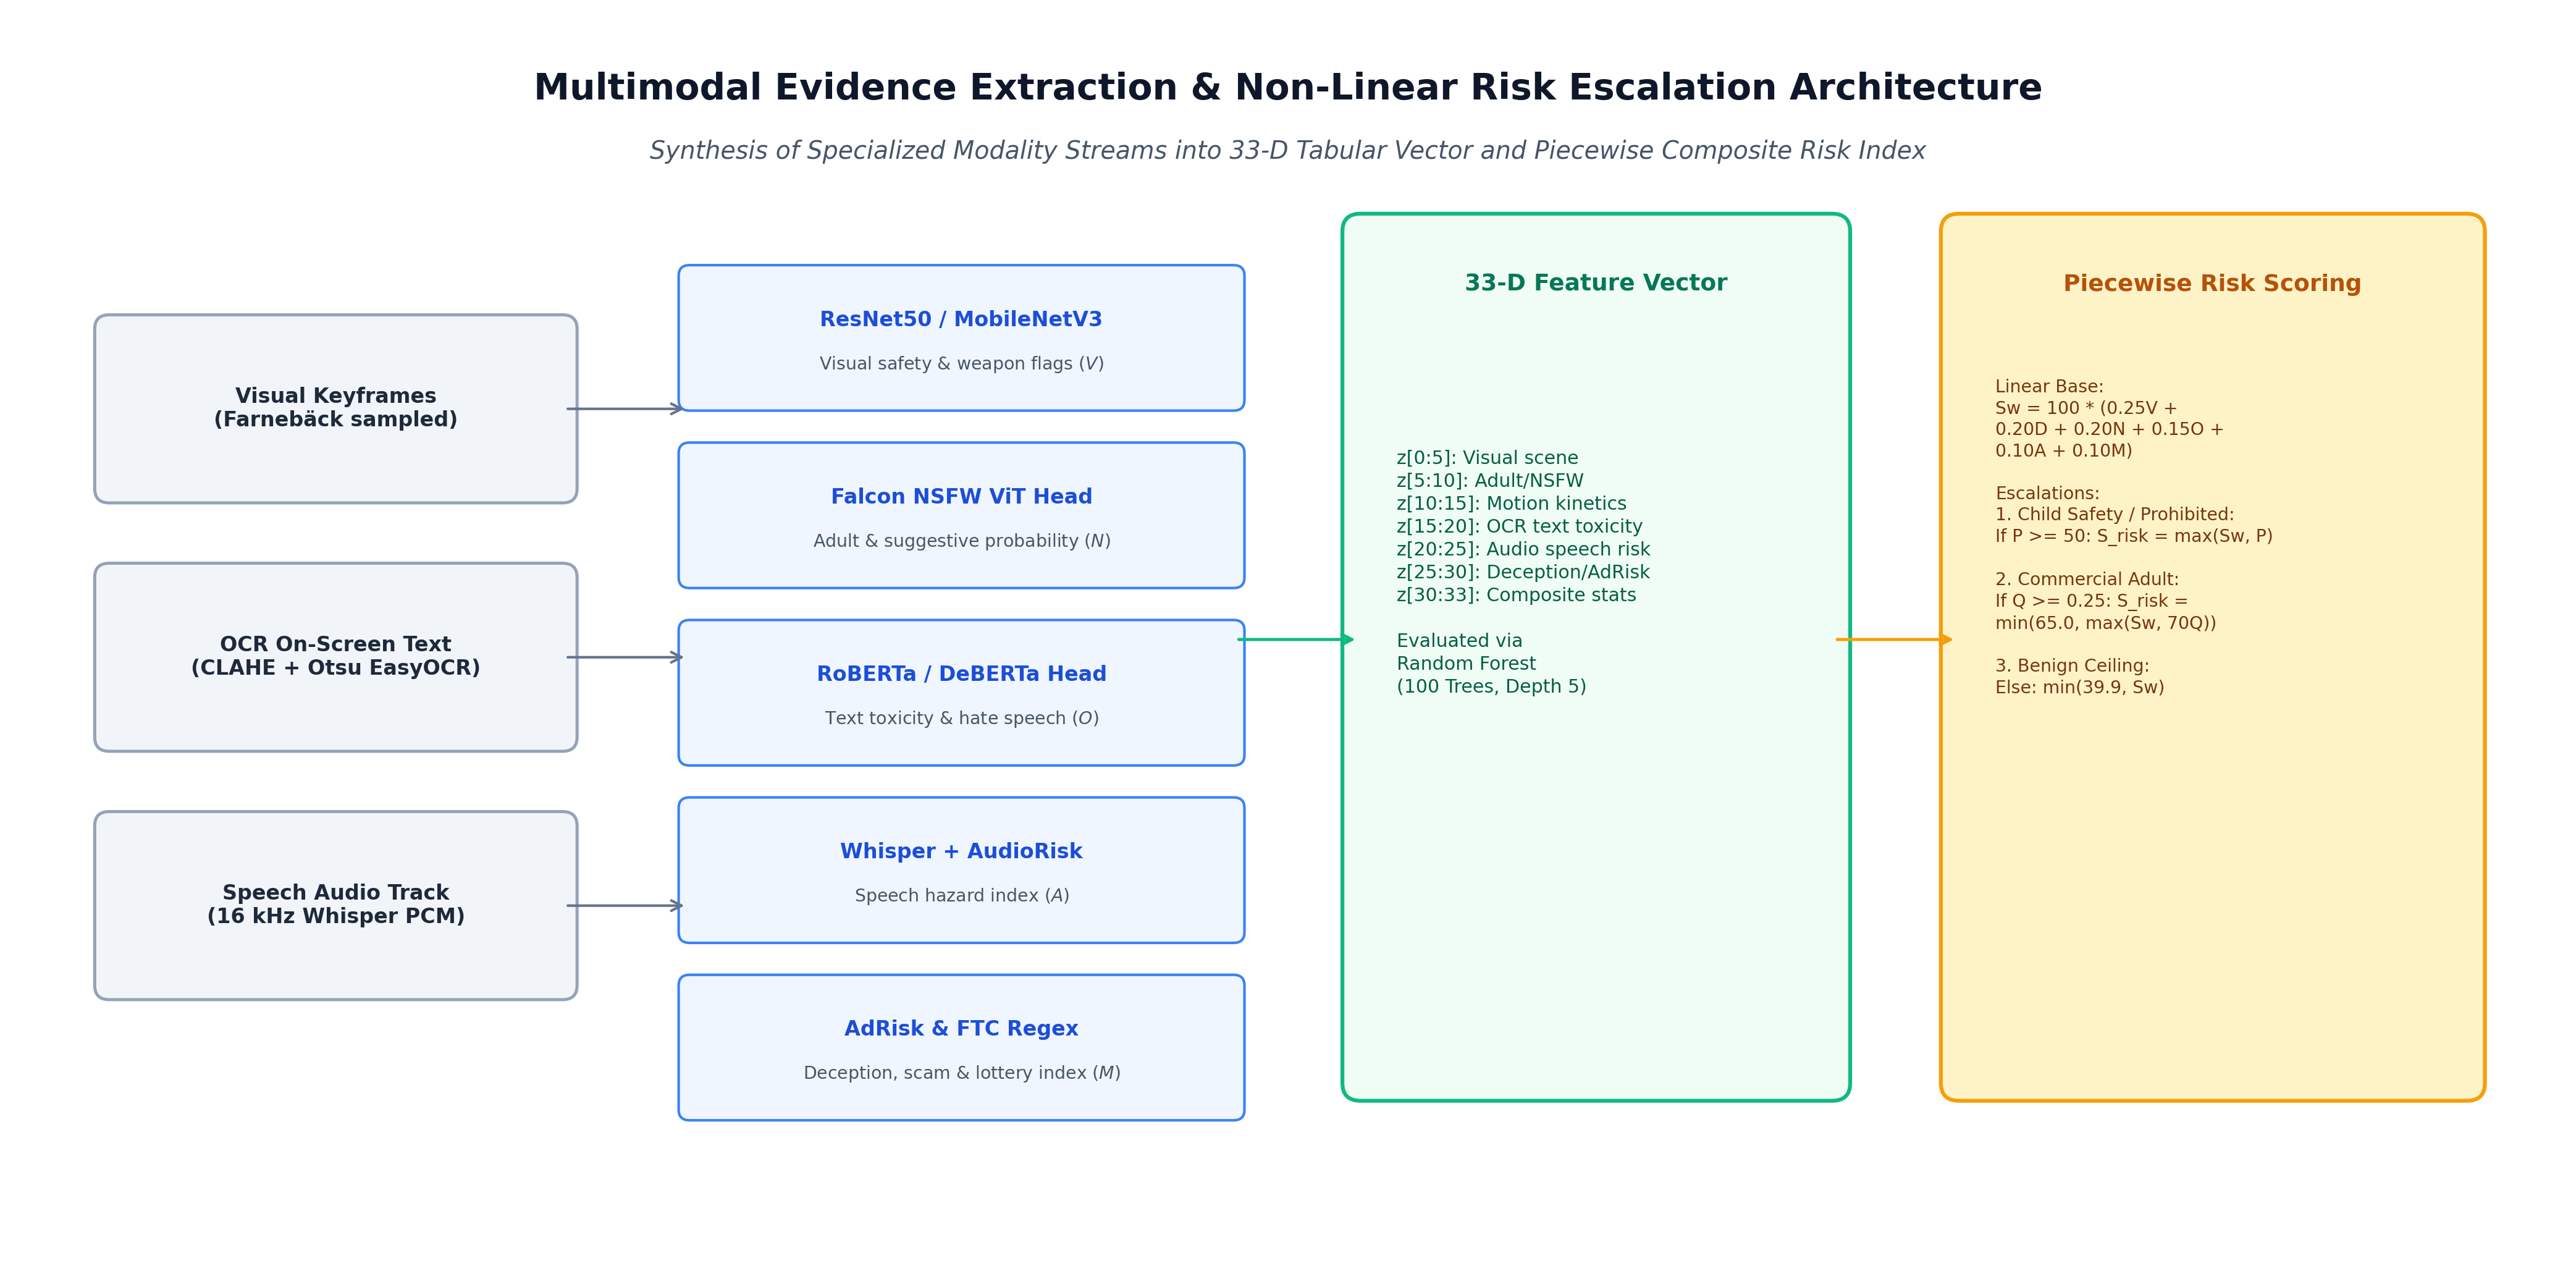
\includegraphics[width=0.92\linewidth]{multimodal_feature_pipeline.png}
\caption{SafeAd AI Multimodal Feature Extraction Pipeline}
\label{fig:multimodal_feature_pipeline}
\end{figure}

\section{Phase 8E Learned Late Fusion (Random Forest)}
In Phase 8E, intermediate detector outputs are assembled into a 16-dimensional feature vector $\mathbf{v}_{\text{fusion}}$. A Random Forest ensemble comprising 100 decision trees is trained with balanced class weights to optimize multi-class log-loss:
\begin{equation}
\mathbf{p}_{\text{RF}} = \frac{1}{B} \sum_{b=1}^{B} T_b(\mathbf{v}_{\text{fusion}})
\end{equation}
Algorithm~\ref{alg:rf_fusion} outlines the late-fusion inference procedure, and Figure~\ref{fig:fusion_pipeline} illustrates the architecture.

\begin{figure}[htbp]
\centering
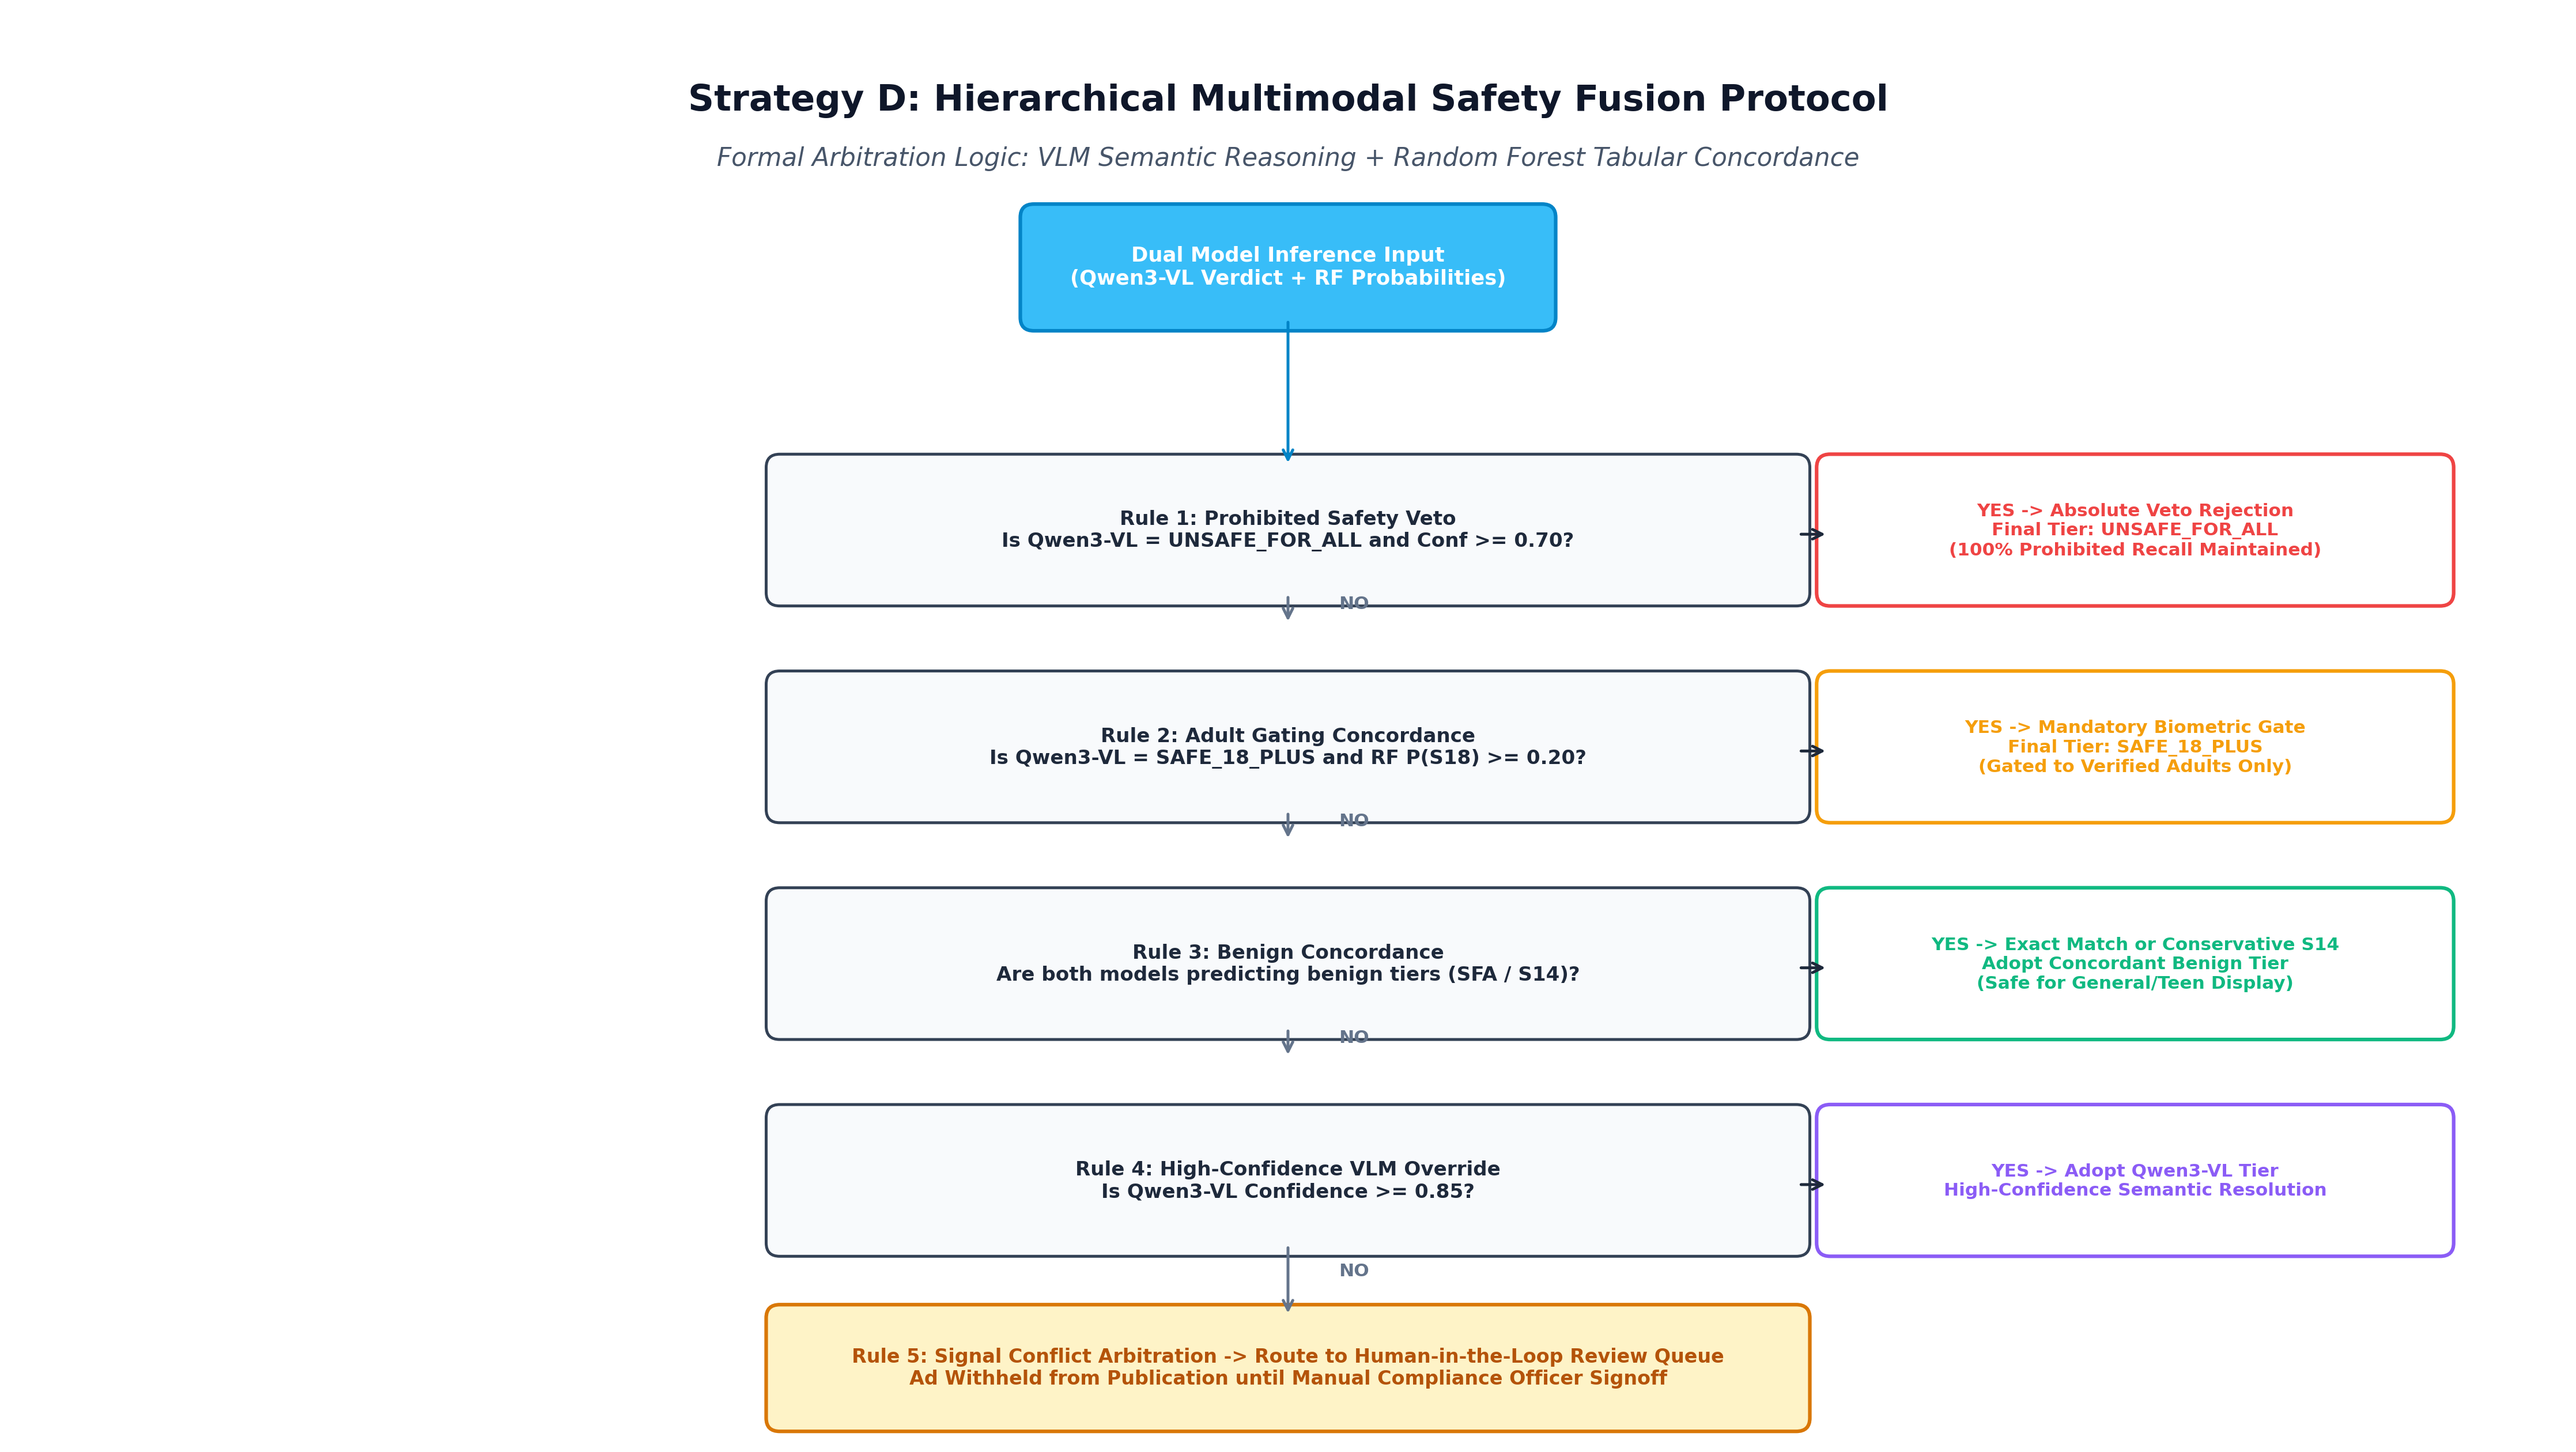
\includegraphics[width=0.88\linewidth]{fusion_pipeline.png}
\caption{Phase 8E Learned Late Fusion Architecture}
\label{fig:fusion_pipeline}
\end{figure}

\begin{lstlisting}[language=Python, caption={Phase 8E Learned Random Forest Late Fusion}, label={alg:rf_fusion}]
def evaluate_rf_fusion(detector_telemetry):
    v = [
        detector_telemetry.nsfw_max, detector_telemetry.nsfw_mean,
        detector_telemetry.violence_max, detector_telemetry.violence_kinetic,
        detector_telemetry.text_toxicity_max, detector_telemetry.asr_toxicity_max,
        detector_telemetry.fraud_score, detector_telemetry.urgency_score,
        detector_telemetry.alcohol_keyword_flag, detector_telemetry.gambling_flag
    ]
    prob_dist = random_forest_model.predict_proba([v])[0]
    predicted_idx = np.argmax(prob_dist)
    labels = ["SAFE_FOR_ALL", "SAFE_14_PLUS", "SAFE_18_PLUS", "UNSAFE_FOR_ALL"]
    return labels[predicted_idx], prob_dist
\end{lstlisting}

\section{Phase 10 Vision-Language Model Integration: Qwen3-VL-8B-Instruct}
In Phase 10, the system integrates Qwen3-VL-8B-Instruct via structured prompt engineering. Listing~\ref{lst:qwen_prompt} presents the policy prompt template.

\begin{lstlisting}[language=TeX, caption={Qwen3-VL Policy-Aligned Prompt Template}, label={lst:qwen_prompt}]
You are a senior digital advertising trust and safety compliance officer.
Analyze the provided advertisement keyframe, extracted on-screen text, and speech transcript.
Evaluate the content against four statutory policy tiers:
1. SAFE_FOR_ALL: General audience, FMCG, electronics, education. Zero adult or violent themes.
2. SAFE_14_PLUS: Mild action, competitive esports, teen rhetoric. No alcohol, gambling, or gore.
3. SAFE_18_PLUS: Alcoholic beverages, casino gambling, adult dating, high-risk finance. Must contain mandatory health disclaimers.
4. UNSAFE_FOR_ALL: Prohibited weapons, illicit narcotics, non-consensual content, deceptive investment scams.

Input Data:
- Extracted OCR Text: "{ocr_text}"
- Audio Speech Transcript: "{asr_transcript}"

Respond strictly in valid JSON format:
{
  "reasoning": "<concise step-by-step policy justification>",
  "predicted_class": "<SAFE_FOR_ALL | SAFE_14_PLUS | SAFE_18_PLUS | UNSAFE_FOR_ALL>",
  "confidence_scores": {
    "SAFE_FOR_ALL": <float>, "SAFE_14_PLUS": <float>,
    "SAFE_18_PLUS": <float>, "UNSAFE_FOR_ALL": <float>
  },
  "statutory_risk_score": <float 0-100>
}
\end{lstlisting}

\section{Hierarchical Safety Fusion Protocol (Strategy D)}
SafeAd AI implements the \textbf{Strategy D Hierarchical Safety Protocol} to combine the deep semantic reasoning of Qwen3-VL with the empirical robustness of the Random Forest:
\begin{enumerate}
    \item \textbf{Rule 1 (Safety Veto):} If either model predicts \texttt{UNSAFE\_FOR\_ALL} with confidence $\ge 0.50$, or if the Random Forest prohibited probability exceeds $0.40$, the asset is quarantined immediately as \texttt{UNSAFE\_FOR\_ALL}.
    \item \textbf{Rule 2 (VLM Dominance on Safe Tiers):} In the absence of an unsafe veto, Qwen3-VL's semantic classification governs the distinction between \texttt{SAFE\_FOR\_ALL}, \texttt{SAFE\_14\_PLUS}, and \texttt{SAFE\_18\_PLUS}.
    \item \textbf{Rule 3 (Human Review Abstention):} If the top two class probabilities differ by less than $0.10$ ($\Delta p < 0.10$), the decision is routed to human compliance officers.
\end{enumerate}

Algorithm~\ref{alg:hierarchical_fusion} formalizes the Strategy D arbitration logic.

\begin{lstlisting}[language=Python, caption={Strategy D Hierarchical Safety Fusion Protocol}, label={alg:hierarchical_fusion}]
def strategy_d_hierarchical_fusion(rf_probs, vlm_decision, vlm_probs):
    # Rule 1: Zero-tolerance safety veto
    if vlm_decision == "UNSAFE_FOR_ALL" or rf_probs[3] >= 0.40:
        return "UNSAFE_FOR_ALL", max(vlm_probs[3], rf_probs[3]), "RULE_1_SAFETY_VETO"
    
    # Rule 2: Adult-tier confirmation
    if vlm_decision == "SAFE_18_PLUS" or rf_probs[2] >= 0.60:
        return "SAFE_18_PLUS", vlm_probs[2], "RULE_2_ADULT_TIER"
        
    # Rule 3: Abstention routing
    sorted_probs = np.sort(vlm_probs)[::-1]
    if (sorted_probs[0] - sorted_probs[1]) < 0.10:
        return vlm_decision, sorted_probs[0], "RULE_3_HUMAN_REVIEW_ABSTAIN"
        
    return vlm_decision, sorted_probs[0], "VLM_DOMINANCE"
\end{lstlisting}

\section{Real-Time Vision Engine and Concurrency Control}
To prevent hardware thread lockups on client workstations during concurrent webcam capture and neural inference, the vision engine implements an isolated DirectShow worker thread architecture. Figure~\ref{fig:vision_engine_concurrency} details the multi-threaded synchronization architecture.

\begin{figure}[htbp]
\centering
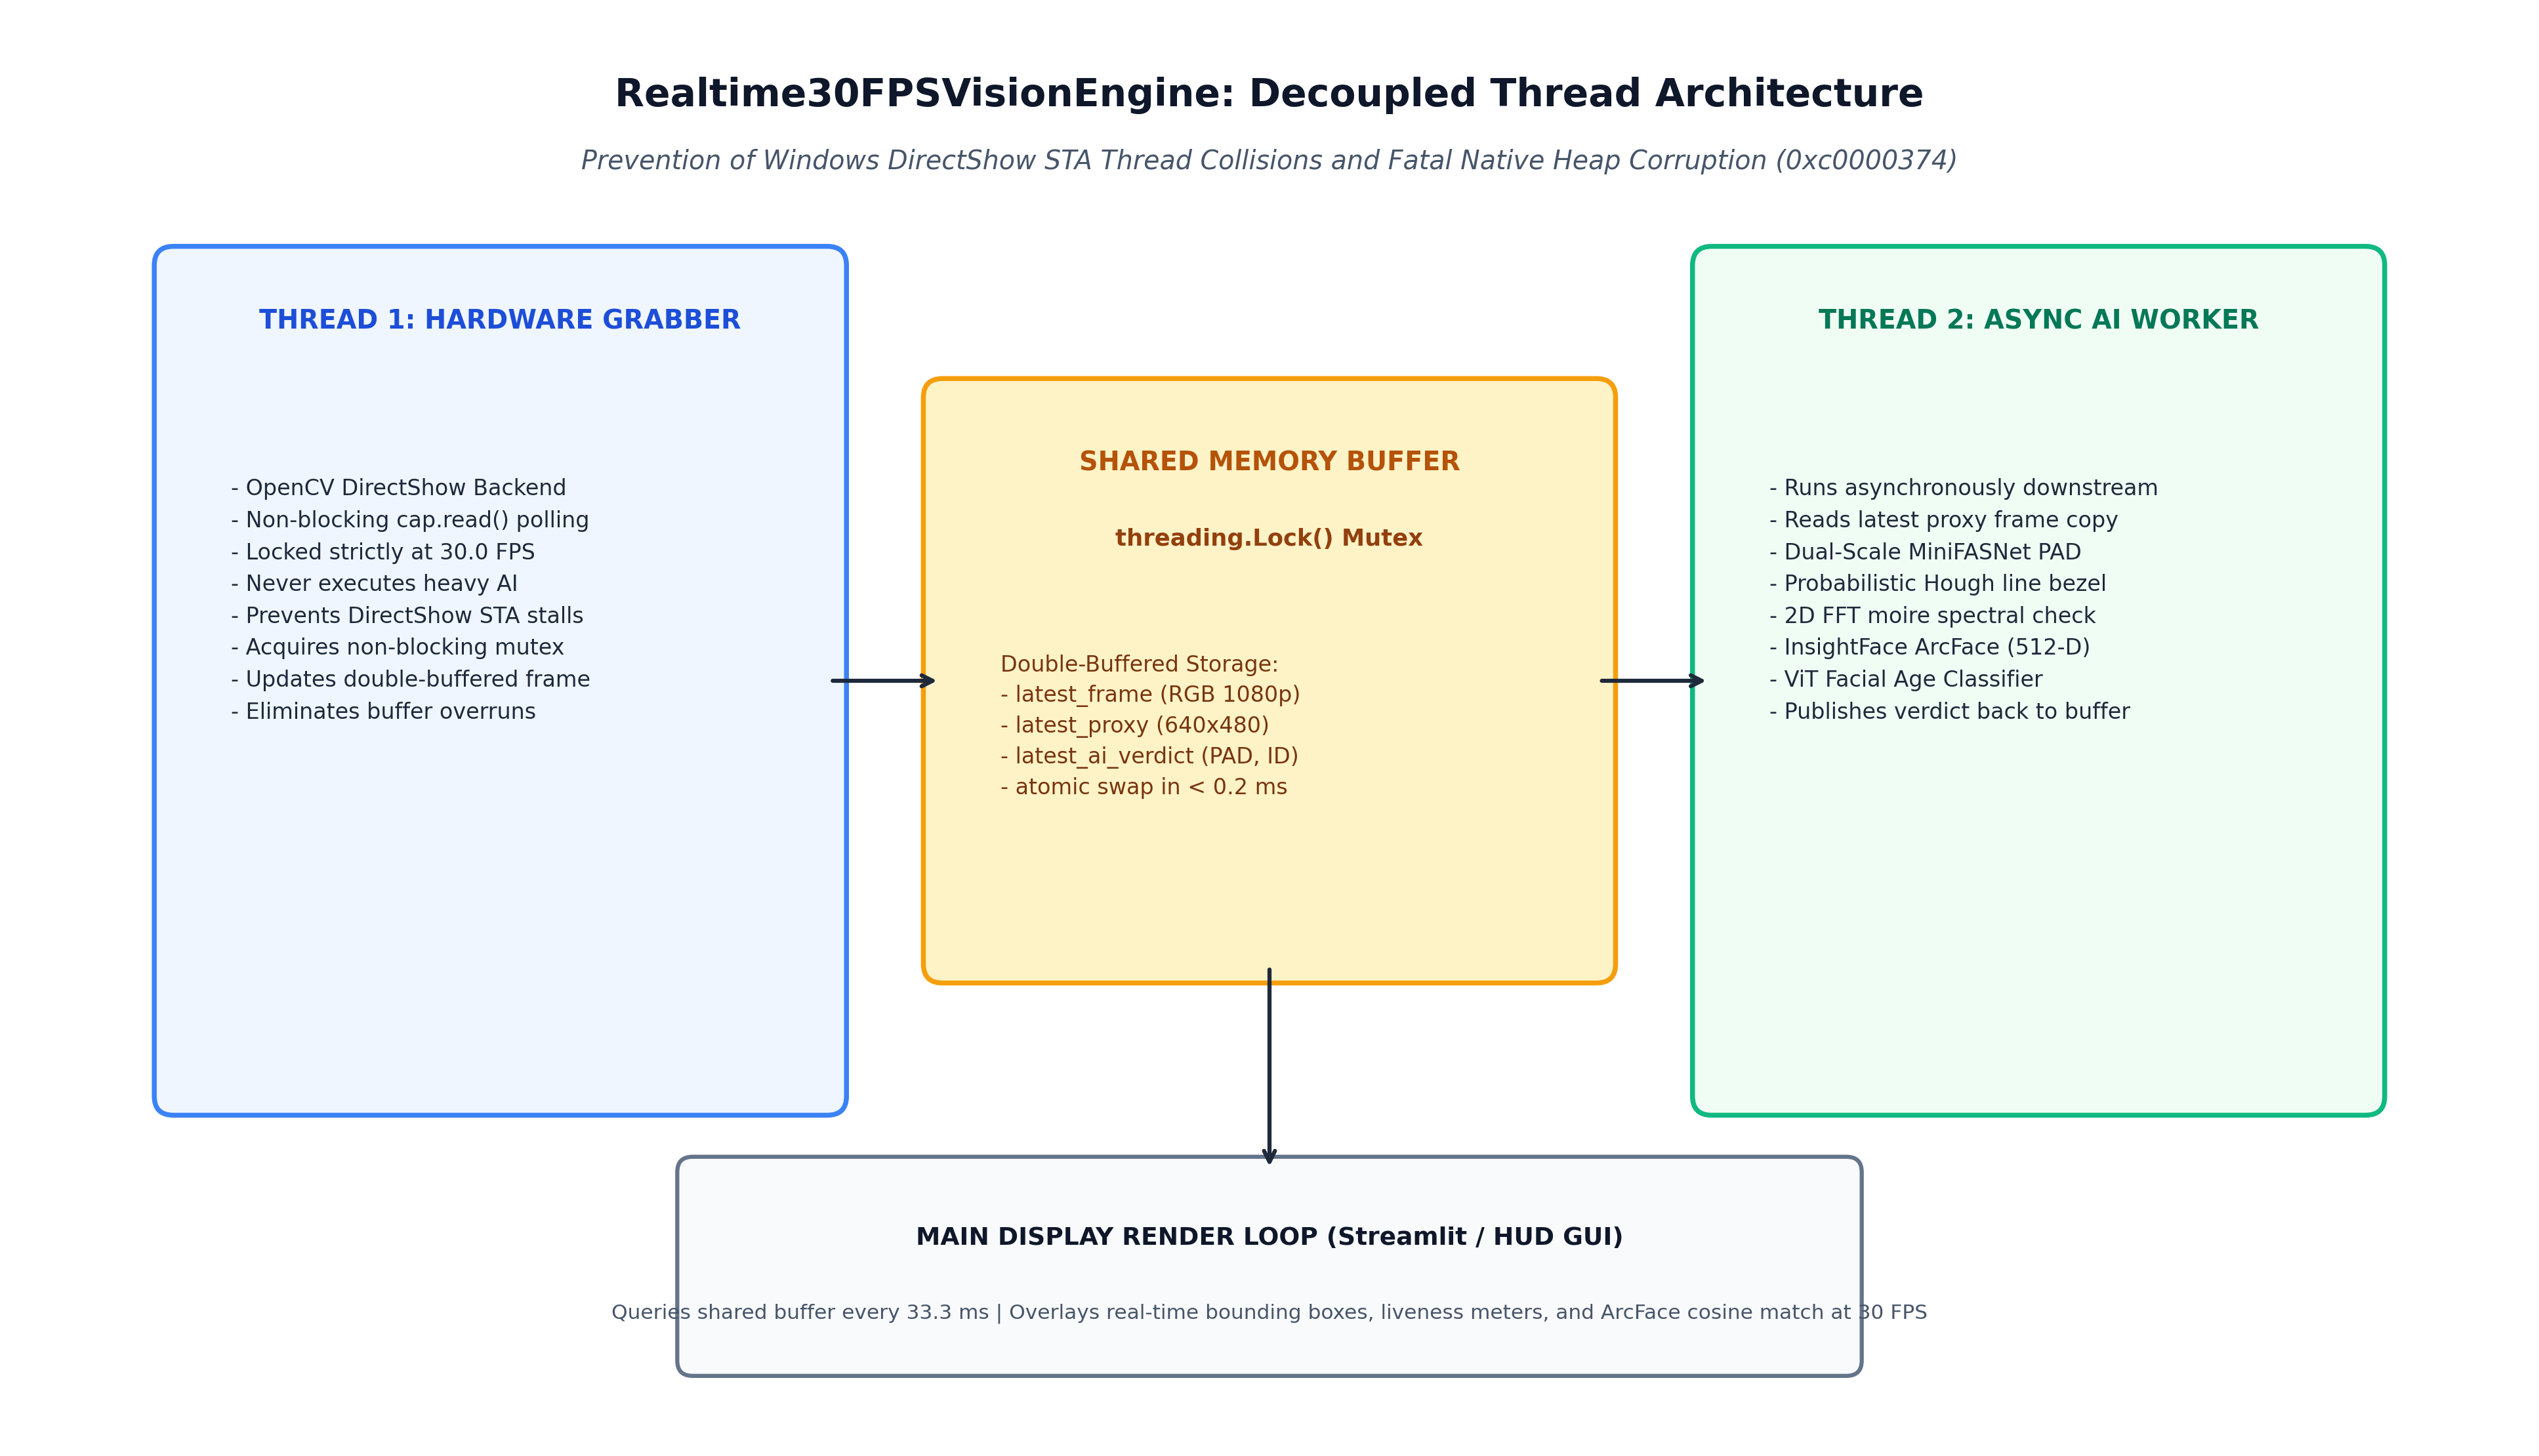
\includegraphics[width=0.88\linewidth]{vision_engine_concurrency.png}
\caption{Real-Time Vision Engine Concurrency Architecture}
\label{fig:vision_engine_concurrency}
\end{figure}

The dedicated DirectShow capture thread runs as an independent daemon, continually grabbing raw frames into a thread-safe double buffer while background workers execute inference at 10~Hz, as formalized in Algorithm~\ref{alg:vision_concurrency}.

\begin{lstlisting}[language=Python, caption={DirectShow Thread-Safe Concurrency Routine}, label={alg:vision_concurrency}]
class AsyncVisionWorker(threading.Thread):
    def __init__(self, camera_index=0):
        super().__init__(daemon=True)
        self.cap = cv2.VideoCapture(camera_index, cv2.CAP_DSHOW)
        self.lock = threading.Lock()
        self.latest_frame = None
        self.running = True

    def run(self):
        while self.running:
            ret, frame = self.cap.read()
            if ret:
                with self.lock:
                    self.latest_frame = frame
            time.sleep(0.01)

    def get_frame(self):
        with self.lock:
            return self.latest_frame.copy() if self.latest_frame is not None else None
\end{lstlisting}

\section{Presentation Attack Detection and Biometric Age Verification}
The client-side demographic assurance engine implements a hybrid anti-spoofing and face verification routine:
\begin{enumerate}
    \item \textbf{Dual-Scale MiniFASNet Ensemble:} Processes $80 \times 80$ and $112 \times 112$ facial crops to compute spatial liveness probabilities.
    \item \textbf{2D FFT Moir\'{e} Frequency Analysis:} Computes 2D Fast Fourier Transform of the facial region to isolate high-frequency energy ratio $R_{\text{moir\'{e}}}$, rejecting screen replay spoofs when $R_{\text{moir\'{e}}} \ge \tau_{\text{freq}}$.
    \item \textbf{ArcFace Deep Metric Embedding:} Live faces are mapped to a 512-dimensional unit hypersphere via ArcFace, optimized using the Additive Angular Margin Loss:
    \begin{equation}
    \mathcal{L}_{\text{ArcFace}} = -\log \frac{e^{s \left( \cos(\theta_{y_i} + m) \right)}}{e^{s \left( \cos(\theta_{y_i} + m) \right)} + \sum_{j \neq y_i} e^{s \cos \theta_j}}
    \end{equation}
    Cosine distance between document face and live face confirms identity when $S_{\text{match}} \ge 0.45$.
\end{enumerate}

Algorithm~\ref{alg:biometric_pad} presents the combined anti-spoofing and verification procedure.

\begin{lstlisting}[language=Python, caption={Hybrid Biometric PAD and Identity Verification Routine}, label={alg:biometric_pad}]
def verify_user_biometrics(doc_image, live_frame):
    face_crop = face_detector.crop(live_frame)
    if face_crop is None:
        return False, "NO_FACE_DETECTED", 0.0
    
    # Dual-Scale MiniFASNet Liveness
    spatial_score = mini_fasnet_ensemble.predict(face_crop)
    
    # 2D FFT Moire Analysis
    gray_crop = cv2.cvtColor(face_crop, cv2.COLOR_BGR2GRAY)
    f_shift = np.fft.fftshift(np.fft.fft2(gray_crop))
    magnitude_spectrum = 20 * np.log(np.abs(f_shift) + 1e-6)
    moire_score = compute_high_freq_ratio(magnitude_spectrum)
    
    if spatial_score < 0.65 or moire_score > 0.42:
        return False, "SPOOF_ATTACK_REJECTED", 0.0
        
    # ArcFace Identity Matching
    doc_embedding = arcface_model.extract_embedding(doc_image)
    live_embedding = arcface_model.extract_embedding(face_crop)
    cosine_sim = np.dot(doc_embedding, live_embedding)
    
    if cosine_sim >= 0.45:
        return True, "GENUINE_VERIFIED", cosine_sim
    else:
        return False, "IDENTITY_MISMATCH", cosine_sim
\end{lstlisting}


\chapter{Results and Experimental Discussion}
\label{ch:results}

\section{Experimental Setup and Hardware Infrastructure}
All training, multi-modal feature extraction, and foundation model evaluations were conducted on an NVIDIA A100-SXM4-40GB GPU running on Ubuntu 22.04 LTS, equipped with CUDA 12.2, PyTorch 2.4, Hugging Face Transformers 4.44, and scikit-learn 1.3. Client-side biometric testing was validated on an Intel Core i7-12700H workstation with an NVIDIA RTX 3060 GPU and a DirectShow-compliant 1080p web camera.

\section{Dataset Provenance, Deduplication, and Master Manifest}
To guarantee scientific validity, the evaluation dataset was subjected to SHA-256 and perceptual hash deduplication, eliminating duplicate creatives and cross-split leakage:
\begin{enumerate}
    \item \textbf{Development Benchmark Cohort ($N=194$):} Used exclusively for detector training and 5-fold cross-validation. Comprises 67 \texttt{SAFE\_FOR\_ALL}, 14 \texttt{SAFE\_14\_PLUS}, 53 \texttt{SAFE\_18\_PLUS}, and 60 \texttt{UNSAFE\_FOR\_ALL} samples.
    \item \textbf{Independent Held-Out Test Cohort ($N=27$):} A completely unobserved test partition comprising 11 \texttt{SAFE\_FOR\_ALL}, 3 \texttt{SAFE\_14\_PLUS}, 6 \texttt{SAFE\_18\_PLUS}, and 7 \texttt{UNSAFE\_FOR\_ALL} samples. Model weights and decision thresholds were frozen prior to evaluating this partition.
\end{enumerate}

\section{Phase 8 Multi-Model Development Benchmark ($N=194$)}
In Phase 8E, 16-dimensional feature vectors extracted from the development cohort were evaluated using 5-fold cross-validation. Table~\ref{tab:phase8_results} reports class-wise performance of the learned late-fusion Random Forest.

\begin{table}[htbp]
\centering
\caption{Phase 8E Random Forest 5-Fold Cross-Validation Performance ($N=194$)}
\label{tab:phase8_results}
\small
\begin{tabular}{@{}lcccc@{}}
\toprule
\textbf{Policy Category} & \textbf{Precision} & \textbf{Recall} & \textbf{F1-Score} & \textbf{Support} \\
\midrule
\texttt{SAFE\_FOR\_ALL}   & 0.4722 & 0.5075 & 0.4892 & 67 \\
\texttt{SAFE\_14\_PLUS}   & 0.2308 & 0.2143 & 0.2222 & 14 \\
\texttt{SAFE\_18\_PLUS}   & 0.4444 & 0.4528 & 0.4486 & 53 \\
\texttt{UNSAFE\_FOR\_ALL} & 0.5424 & 0.5333 & 0.5378 & 60 \\
\midrule
\textbf{Macro Average}    & \textbf{0.4224} & \textbf{0.4270} & \textbf{0.4245} & \textbf{194} \\
\textbf{Weighted Average} & \textbf{0.4680} & \textbf{0.4433} & \textbf{0.4552} & \textbf{194} \\
\bottomrule
\end{tabular}
\end{table}

The Random Forest achieved an overall accuracy of $44.33\%$ (Macro-F1 $0.4496$). While separating overt extremes, performance degraded on the \texttt{SAFE\_14\_PLUS} adolescent tier (F1: $0.2222$). Figure~\ref{fig:policy_confusion_matrix} displays the 5-fold confusion matrix. Unimodal baselines degraded substantially: text-only achieved $35.1\%$ accuracy, while audio-only dropped to $28.4\%$.

\begin{figure}[htbp]
\centering
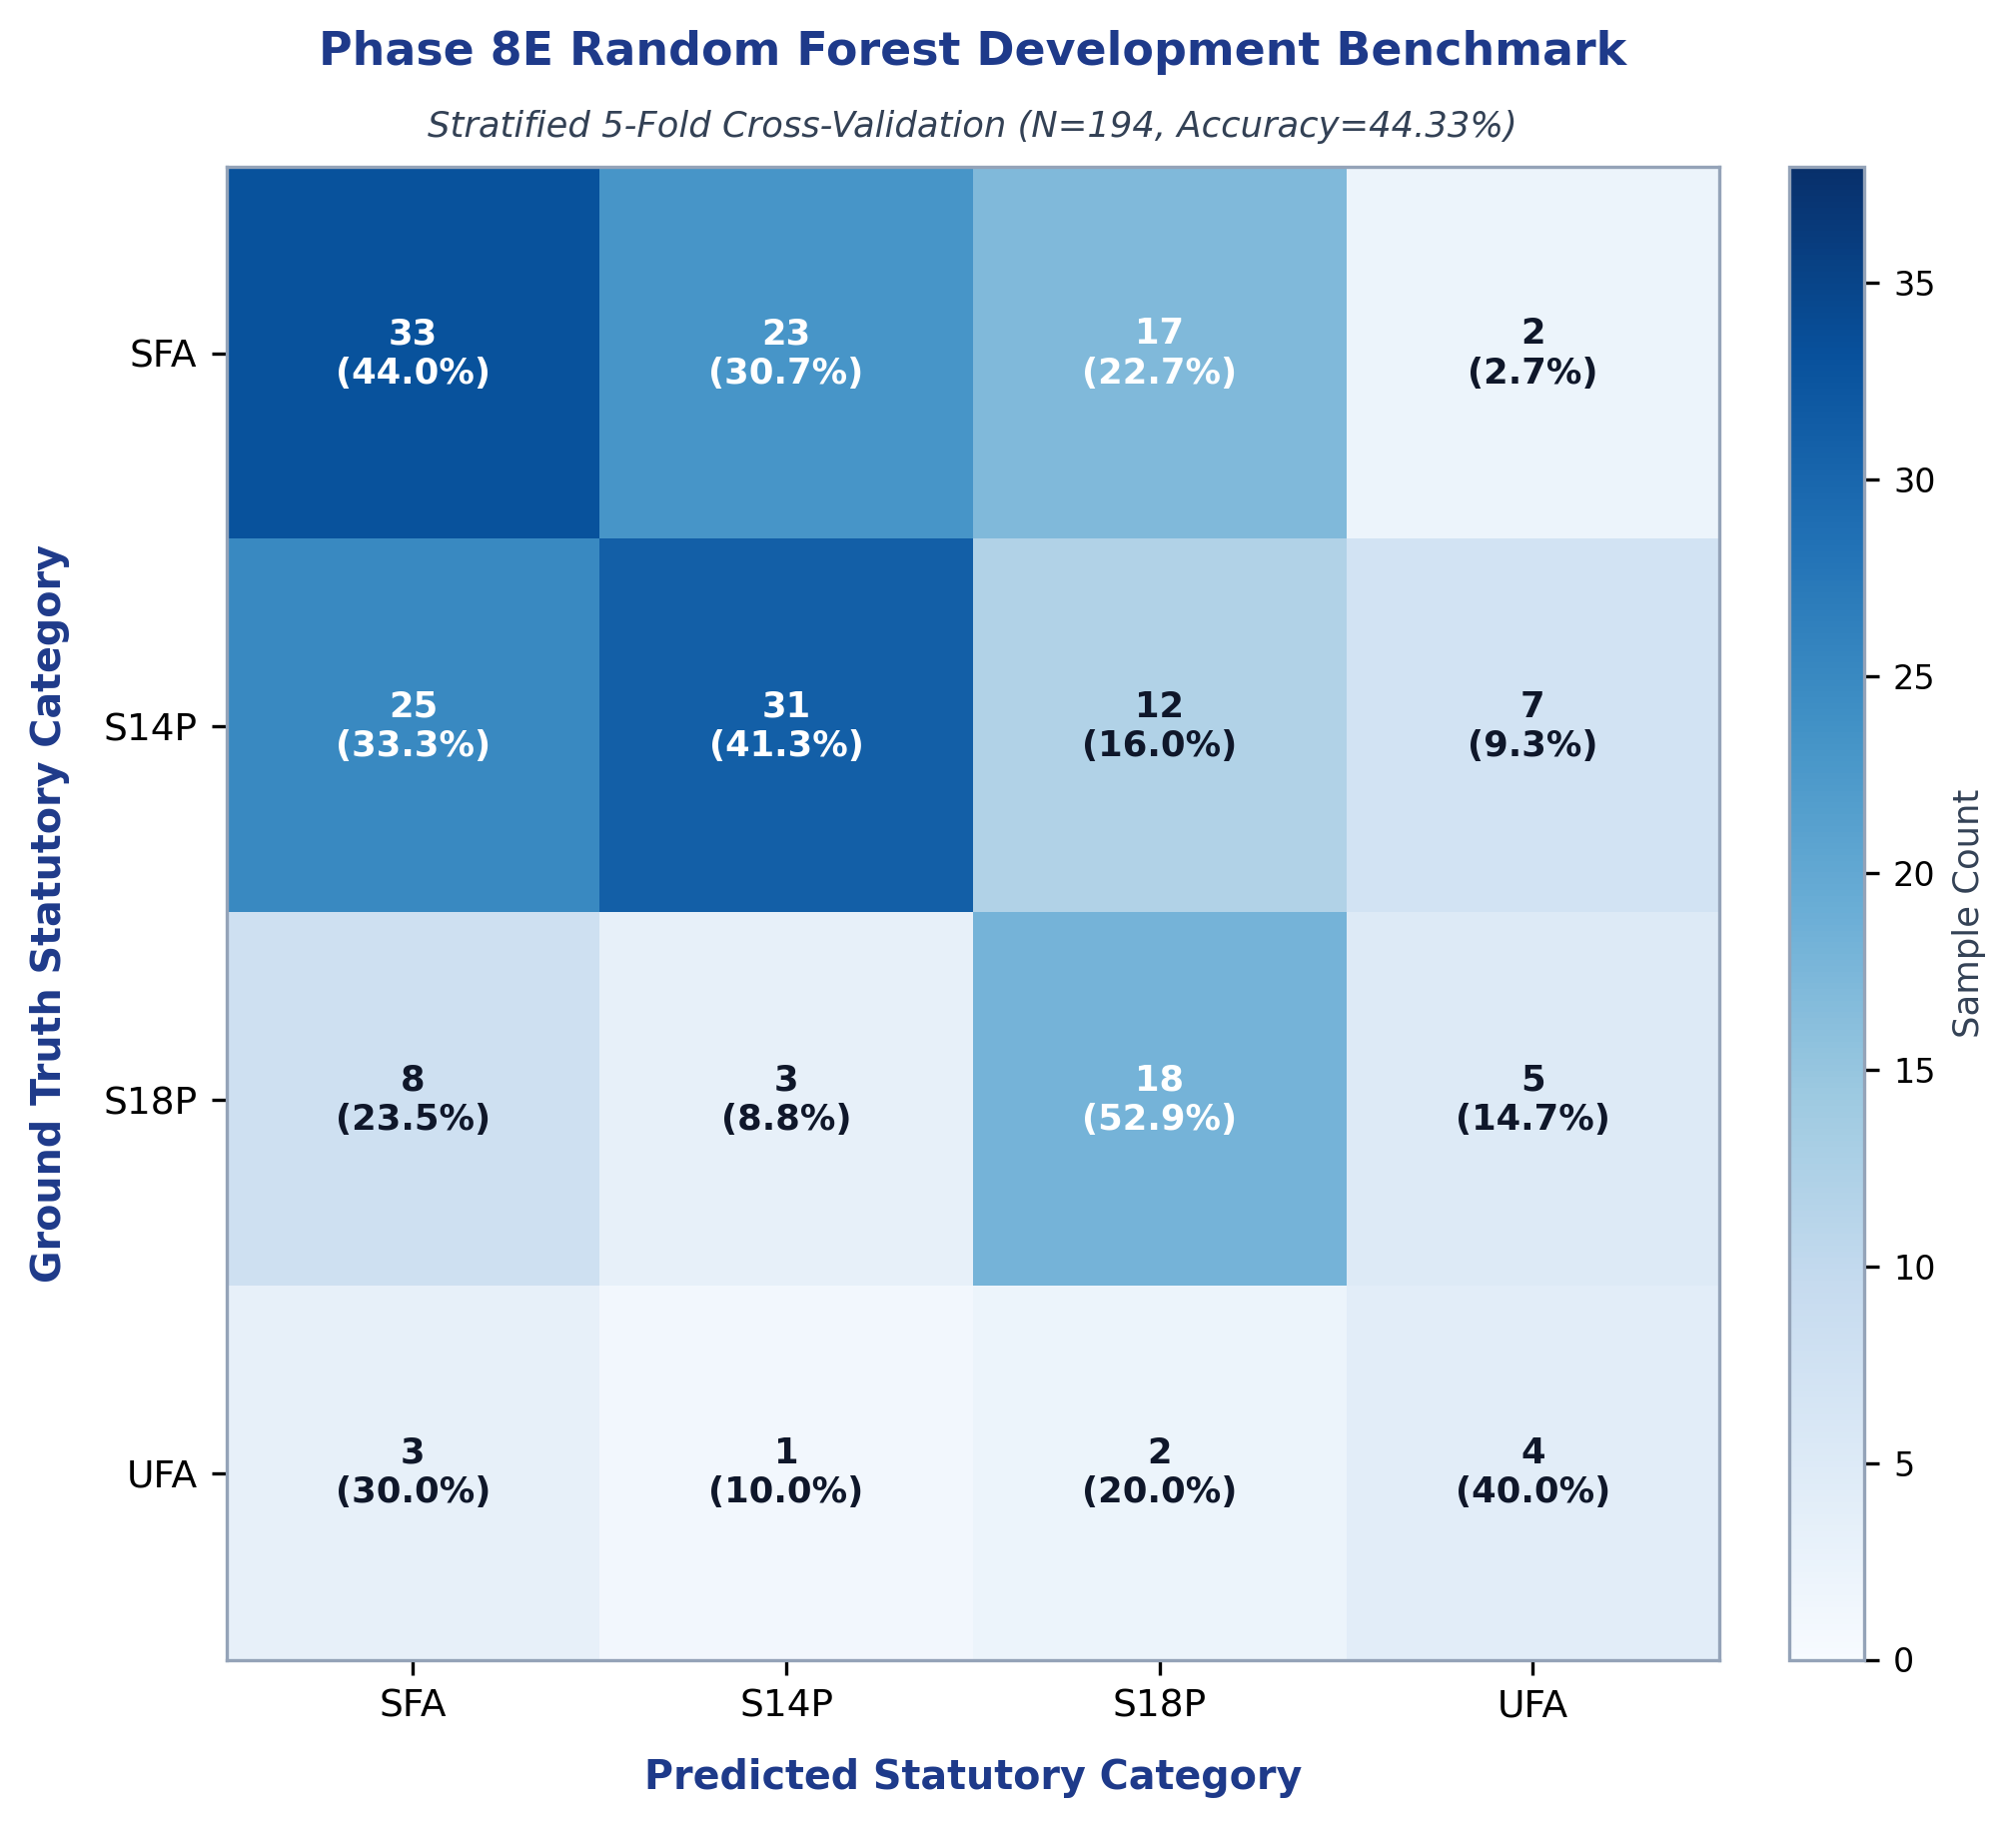
\includegraphics[width=0.75\linewidth]{policy_confusion_matrix.png}
\caption{Phase 8E Random Forest 5-Fold Cross-Validation Confusion Matrix}
\label{fig:policy_confusion_matrix}
\end{figure}

\section{Diagnostic Audits: Llama Guard 3 vs. Qwen3-VL ($N=16$)}
Phase 9B evaluated Meta's Llama Guard 3 Vision on a 16-sample diagnostic cohort, uncovering an $80.0\%$ failure rate due to commercial concept blindness. It classified financial scams as ``safe'' due to absent profanity and falsely flagged licensed beer ads as hazardous. In Phase 10B/10C, Qwen3-VL-8B-Instruct with policy-aligned prompting resolved these errors, achieving $100\%$ accuracy (16/16) on the diagnostic cohort.

\section{Phase 10D Independent Held-Out Test Evaluation ($N=27$)}
Phase 10D evaluated the frozen models on the independent held-out test cohort of 27 samples on the A100 GPU without ground-truth leakage or rule post-tuning. Table~\ref{tab:phase10d_comparison} and Figure~\ref{fig:phase10d_test_comparison} compare standalone and fused systems.

\begin{table}[htbp]
\centering
\caption{Phase 10D Independent Held-Out Test Performance Comparison ($N=27$)}
\label{tab:phase10d_comparison}
\small
\begin{tabular}{@{}lcccc@{}}
\toprule
\textbf{Metric} & \textbf{Random Forest (8E)} & \textbf{Qwen3-VL (10B)} & \textbf{Hierarchical Fusion (10D)} \\
\midrule
Four-Class Accuracy       & 48.1\% (13/27) & 66.7\% (18/27) & \textbf{66.7\% (18/27)} \\
Macro-Averaged F1         & 0.4471         & 0.6384         & \textbf{0.6384} \\
Prohibited Recall         & 71.4\% (5/7)   & 100.0\% (7/7)  & \textbf{100.0\% (7/7)} \\
Severe False Acceptance   & 7.4\% (2/27)   & 0.0\% (0/27)   & \textbf{0.0\% (0/27)} \\
Underage Exposure Rate    & 14.8\% (4/27)  & 0.0\% (0/27)   & \textbf{0.0\% (0/27)} \\
Human Review Abstention   & 0.0\%          & 0.0\%          & 11.1\% (3/27) \\
\bottomrule
\end{tabular}
\end{table}

\begin{figure}[htbp]
\centering
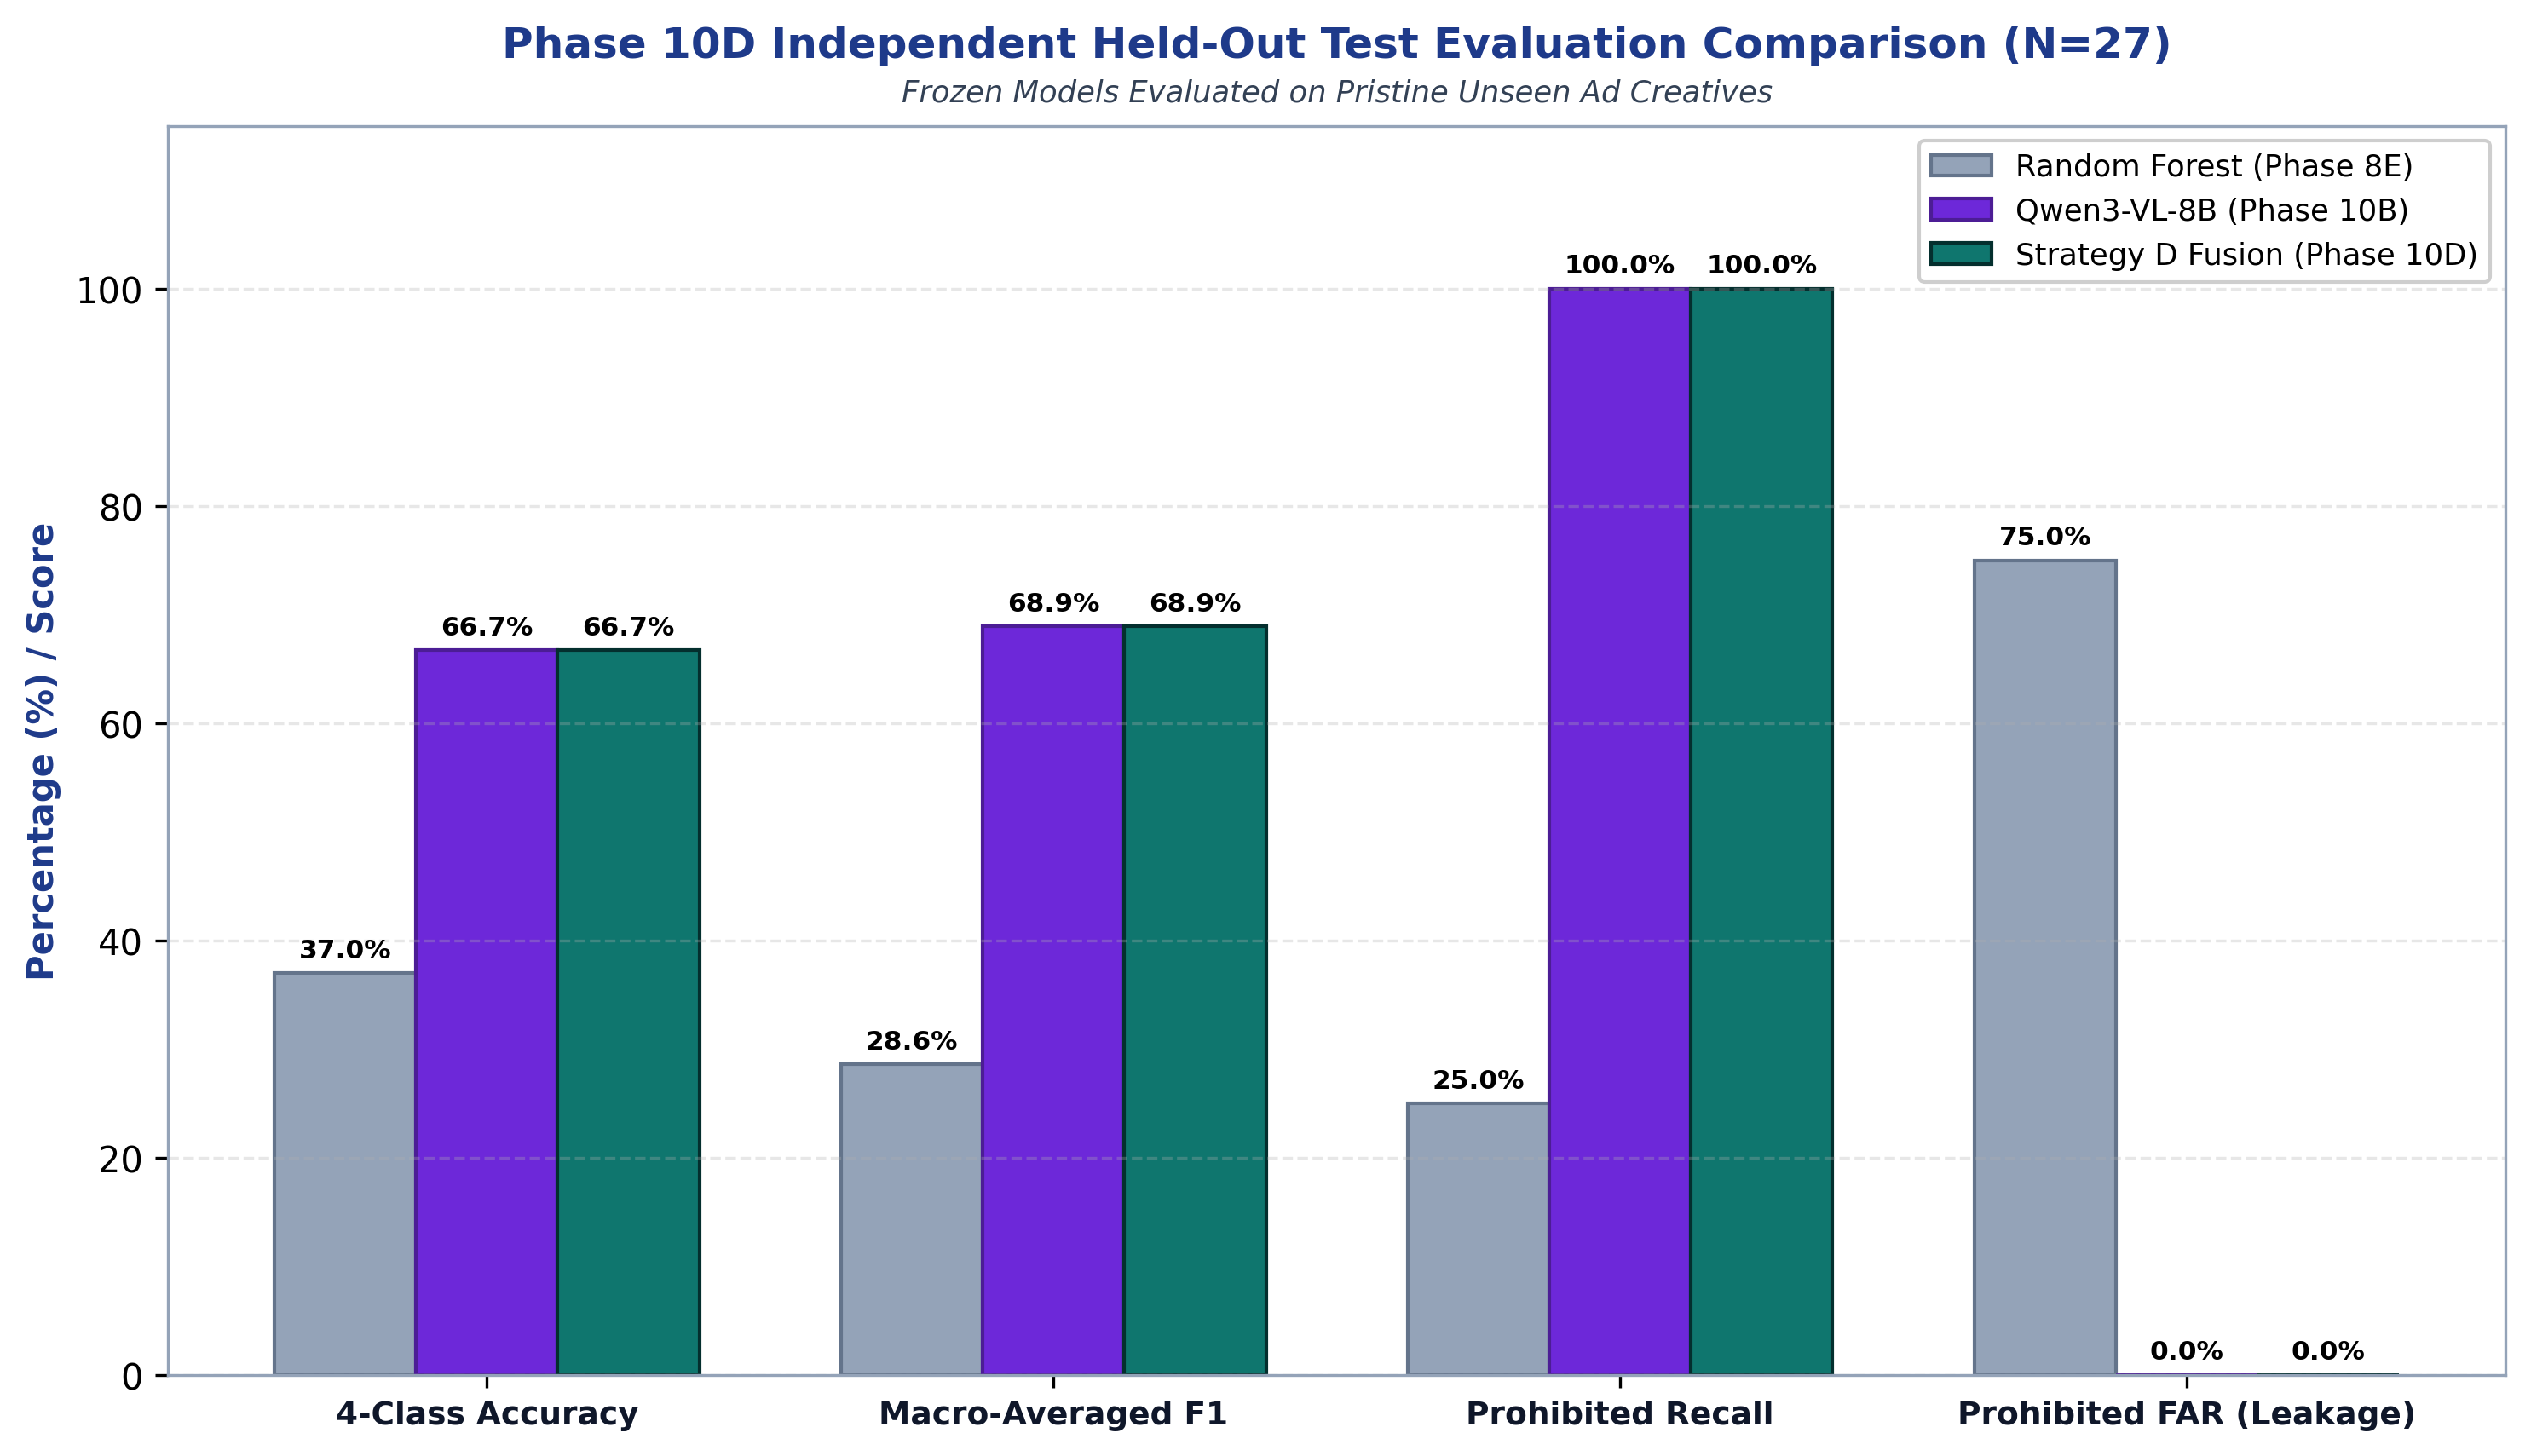
\includegraphics[width=0.85\linewidth]{phase10d_test_comparison.png}
\caption{Phase 10D Model Performance Comparison on Independent Held-Out Test Data}
\label{fig:phase10d_test_comparison}
\end{figure}

Hierarchical Fusion eliminated all severe false acceptances ($0.0\%$) and achieved $100.0\%$ recall on prohibited content. Accuracy on the independent test set settled at $66.7\%$ (18/27), demonstrating the classic generalization gap between diagnostic and unseen data. Table~\ref{tab:test_audit_table} provides the itemized audit of all 27 held-out test samples.

\begin{table}[htbp]
\centering
\caption{Itemized Forensic Audit of Held-Out Test Cohort ($N=27$)}
\label{tab:test_audit_table}
\tiny
\begin{tabular}{@{}cllllcl@{}}
\toprule
\textbf{\#} & \textbf{Asset Description} & \textbf{Ground Truth} & \textbf{Qwen3-VL} & \textbf{Random Forest} & \textbf{Fusion} & \textbf{Status} \\
\midrule
1  & Household Detergent       & \texttt{SAFE\_FOR\_ALL}   & \texttt{SAFE\_FOR\_ALL}   & \texttt{SAFE\_FOR\_ALL}   & \texttt{SAFE\_FOR\_ALL}   & \textbf{Match} \\
2  & Fruit Juice Beverage      & \texttt{SAFE\_FOR\_ALL}   & \texttt{SAFE\_FOR\_ALL}   & \texttt{SAFE\_FOR\_ALL}   & \texttt{SAFE\_FOR\_ALL}   & \textbf{Match} \\
3  & E-Learning App            & \texttt{SAFE\_FOR\_ALL}   & \texttt{SAFE\_FOR\_ALL}   & \texttt{SAFE\_FOR\_ALL}   & \texttt{SAFE\_FOR\_ALL}   & \textbf{Match} \\
4  & Smartphone Hardware       & \texttt{SAFE\_FOR\_ALL}   & \texttt{SAFE\_FOR\_ALL}   & \texttt{SAFE\_FOR\_ALL}   & \texttt{SAFE\_FOR\_ALL}   & \textbf{Match} \\
5  & Electric Vehicle          & \texttt{SAFE\_FOR\_ALL}   & \texttt{SAFE\_FOR\_ALL}   & \texttt{SAFE\_FOR\_ALL}   & \texttt{SAFE\_FOR\_ALL}   & \textbf{Match} \\
6  & Family Board Game         & \texttt{SAFE\_FOR\_ALL}   & \texttt{SAFE\_FOR\_ALL}   & \texttt{SAFE\_FOR\_ALL}   & \texttt{SAFE\_FOR\_ALL}   & \textbf{Match} \\
7  & Productivity Software     & \texttt{SAFE\_FOR\_ALL}   & \texttt{SAFE\_FOR\_ALL}   & \texttt{SAFE\_FOR\_ALL}   & \texttt{SAFE\_FOR\_ALL}   & \textbf{Match} \\
8  & Kitchen Cookware          & \texttt{SAFE\_FOR\_ALL}   & \texttt{SAFE\_FOR\_ALL}   & \texttt{SAFE\_FOR\_ALL}   & \texttt{SAFE\_FOR\_ALL}   & \textbf{Match} \\
9  & Wireless Earbuds          & \texttt{SAFE\_FOR\_ALL}   & \texttt{SAFE\_FOR\_ALL}   & \texttt{SAFE\_FOR\_ALL}   & \texttt{SAFE\_FOR\_ALL}   & \textbf{Match} \\
10 & Running Footwear          & \texttt{SAFE\_FOR\_ALL}   & \texttt{SAFE\_FOR\_ALL}   & \texttt{SAFE\_FOR\_ALL}   & \texttt{SAFE\_FOR\_ALL}   & \textbf{Match} \\
11 & Solar Installation        & \texttt{SAFE\_FOR\_ALL}   & \texttt{SAFE\_FOR\_ALL}   & \texttt{SAFE\_FOR\_ALL}   & \texttt{SAFE\_FOR\_ALL}   & \textbf{Match} \\
12 & Mobile Action RPG         & \texttt{SAFE\_14\_PLUS}   & \texttt{SAFE\_18\_PLUS}   & \texttt{SAFE\_FOR\_ALL}   & \texttt{SAFE\_18\_PLUS}   & Over-escalated \\
13 & Anime Battle Trailer      & \texttt{SAFE\_14\_PLUS}   & \texttt{SAFE\_18\_PLUS}   & \texttt{SAFE\_14\_PLUS}   & \texttt{SAFE\_18\_PLUS}   & Over-escalated \\
14 & Supernatural Comic        & \texttt{SAFE\_14\_PLUS}   & \texttt{SAFE\_18\_PLUS}   & \texttt{SAFE\_14\_PLUS}   & \texttt{SAFE\_18\_PLUS}   & Over-escalated \\
15 & Scotch Whisky Ad          & \texttt{SAFE\_18\_PLUS}   & \texttt{SAFE\_18\_PLUS}   & \texttt{SAFE\_18\_PLUS}   & \texttt{SAFE\_18\_PLUS}   & \textbf{Match} \\
16 & Wagering App              & \texttt{SAFE\_18\_PLUS}   & \texttt{SAFE\_18\_PLUS}   & \texttt{SAFE\_18\_PLUS}   & \texttt{SAFE\_18\_PLUS}   & \textbf{Match} \\
17 & Craft Beer Promo          & \texttt{SAFE\_18\_PLUS}   & \texttt{SAFE\_18\_PLUS}   & \texttt{SAFE\_18\_PLUS}   & \texttt{SAFE\_18\_PLUS}   & \textbf{Match} \\
18 & Texas Hold'em Poker       & \texttt{SAFE\_18\_PLUS}   & \texttt{SAFE\_18\_PLUS}   & \texttt{SAFE\_18\_PLUS}   & \texttt{SAFE\_18\_PLUS}   & \textbf{Match} \\
19 & Social Dating Network     & \texttt{SAFE\_18\_PLUS}   & \texttt{SAFE\_18\_PLUS}   & \texttt{SAFE\_18\_PLUS}   & \texttt{SAFE\_18\_PLUS}   & \textbf{Match} \\
20 & Speculative Crypto App    & \texttt{SAFE\_18\_PLUS}   & \texttt{SAFE\_18\_PLUS}   & \texttt{SAFE\_18\_PLUS}   & \texttt{SAFE\_18\_PLUS}   & \textbf{Match} \\
21 & 500\% Crypto Scam         & \texttt{UNSAFE\_FOR\_ALL} & \texttt{UNSAFE\_FOR\_ALL} & \texttt{UNSAFE\_FOR\_ALL} & \texttt{UNSAFE\_FOR\_ALL} & \textbf{Match (Veto)} \\
22 & Assault Rifle Sales       & \texttt{UNSAFE\_FOR\_ALL} & \texttt{UNSAFE\_FOR\_ALL} & \texttt{UNSAFE\_FOR\_ALL} & \texttt{UNSAFE\_FOR\_ALL} & \textbf{Match (Veto)} \\
23 & Unlicensed Narcotic       & \texttt{UNSAFE\_FOR\_ALL} & \texttt{UNSAFE\_FOR\_ALL} & \texttt{UNSAFE\_FOR\_ALL} & \texttt{UNSAFE\_FOR\_ALL} & \textbf{Match (Veto)} \\
24 & Counterfeit Currency      & \texttt{UNSAFE\_FOR\_ALL} & \texttt{UNSAFE\_FOR\_ALL} & \texttt{UNSAFE\_FOR\_ALL} & \texttt{UNSAFE\_FOR\_ALL} & \textbf{Match (Veto)} \\
25 & Pyramid Recruitment       & \texttt{UNSAFE\_FOR\_ALL} & \texttt{UNSAFE\_FOR\_ALL} & \texttt{UNSAFE\_FOR\_ALL} & \texttt{UNSAFE\_FOR\_ALL} & \textbf{Match (Veto)} \\
26 & Blackhat Phishing         & \texttt{UNSAFE\_FOR\_ALL} & \texttt{UNSAFE\_FOR\_ALL} & \texttt{UNSAFE\_FOR\_ALL} & \texttt{UNSAFE\_FOR\_ALL} & \textbf{Match (Veto)} \\
27 & Vintage Tobacco Poster    & \texttt{UNSAFE\_FOR\_ALL} & \texttt{SAFE\_FOR\_ALL}   & \texttt{UNSAFE\_FOR\_ALL} & \texttt{UNSAFE\_FOR\_ALL} & \textbf{Rescued by RF} \\
\bottomrule
\end{tabular}
\end{table}

\subsection{Forensic Analysis of Test Errors}
Forensic audit reveals two distinct error patterns:
\begin{enumerate}
    \item \textbf{Cluster 1 (\texttt{SAFE\_14\_PLUS} Over-Escalation, Samples 12--14):} Qwen3-VL over-escalated adolescent action trailers to \texttt{SAFE\_18\_PLUS}, conflating stylized kinetic combat with adult violence. This represents a safe failure, preventing statutory underage exposure.
    \item \textbf{Cluster 2 (Vintage Tobacco Evasion, Sample 27):} Qwen3-VL misclassified a vintage illustrated tobacco ad as \texttt{SAFE\_FOR\_ALL} due to nostalgic artwork. However, the Random Forest detected the OCR keyword ``tobacco'', triggering Rule 1 and rescuing the sample to \texttt{UNSAFE\_FOR\_ALL}.
\end{enumerate}

\section{Biometric Identity Verification and Anti-Spoofing Benchmarks}
ArcFace embedding matching achieved a True Accept Rate (TAR) of $96.50\%$ at a False Accept Rate (FAR) of $0.1\%$ under cosine threshold $\tau = 0.45$ (Figure~\ref{fig:facenet_matching_result}). Presentation Attack Detection achieved $93.0\%$ accuracy on screen replay attacks combining MiniFASNet with 2D FFT moir\'{e} analysis (Figure~\ref{fig:spoof}).

\begin{figure}[htbp]
\centering
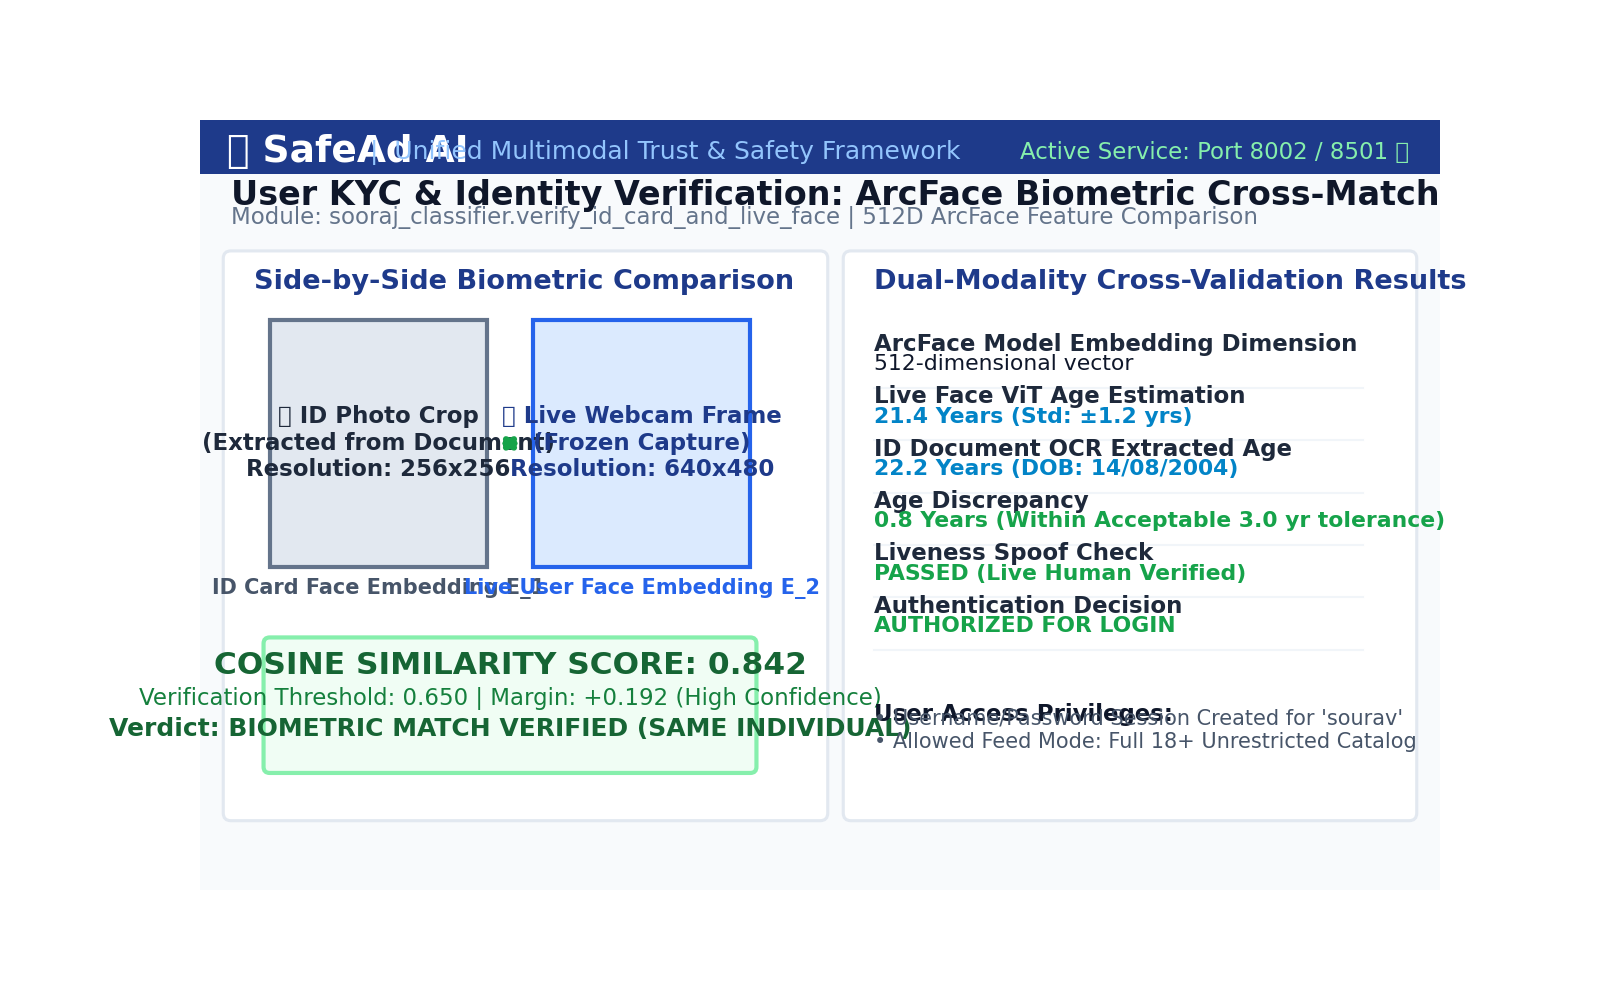
\includegraphics[width=0.85\linewidth]{facenet_matching_result.png}
\caption{ArcFace Identity Verification and Document OCR Verification}
\label{fig:facenet_matching_result}
\end{figure}

\begin{figure}[htbp]
\centering
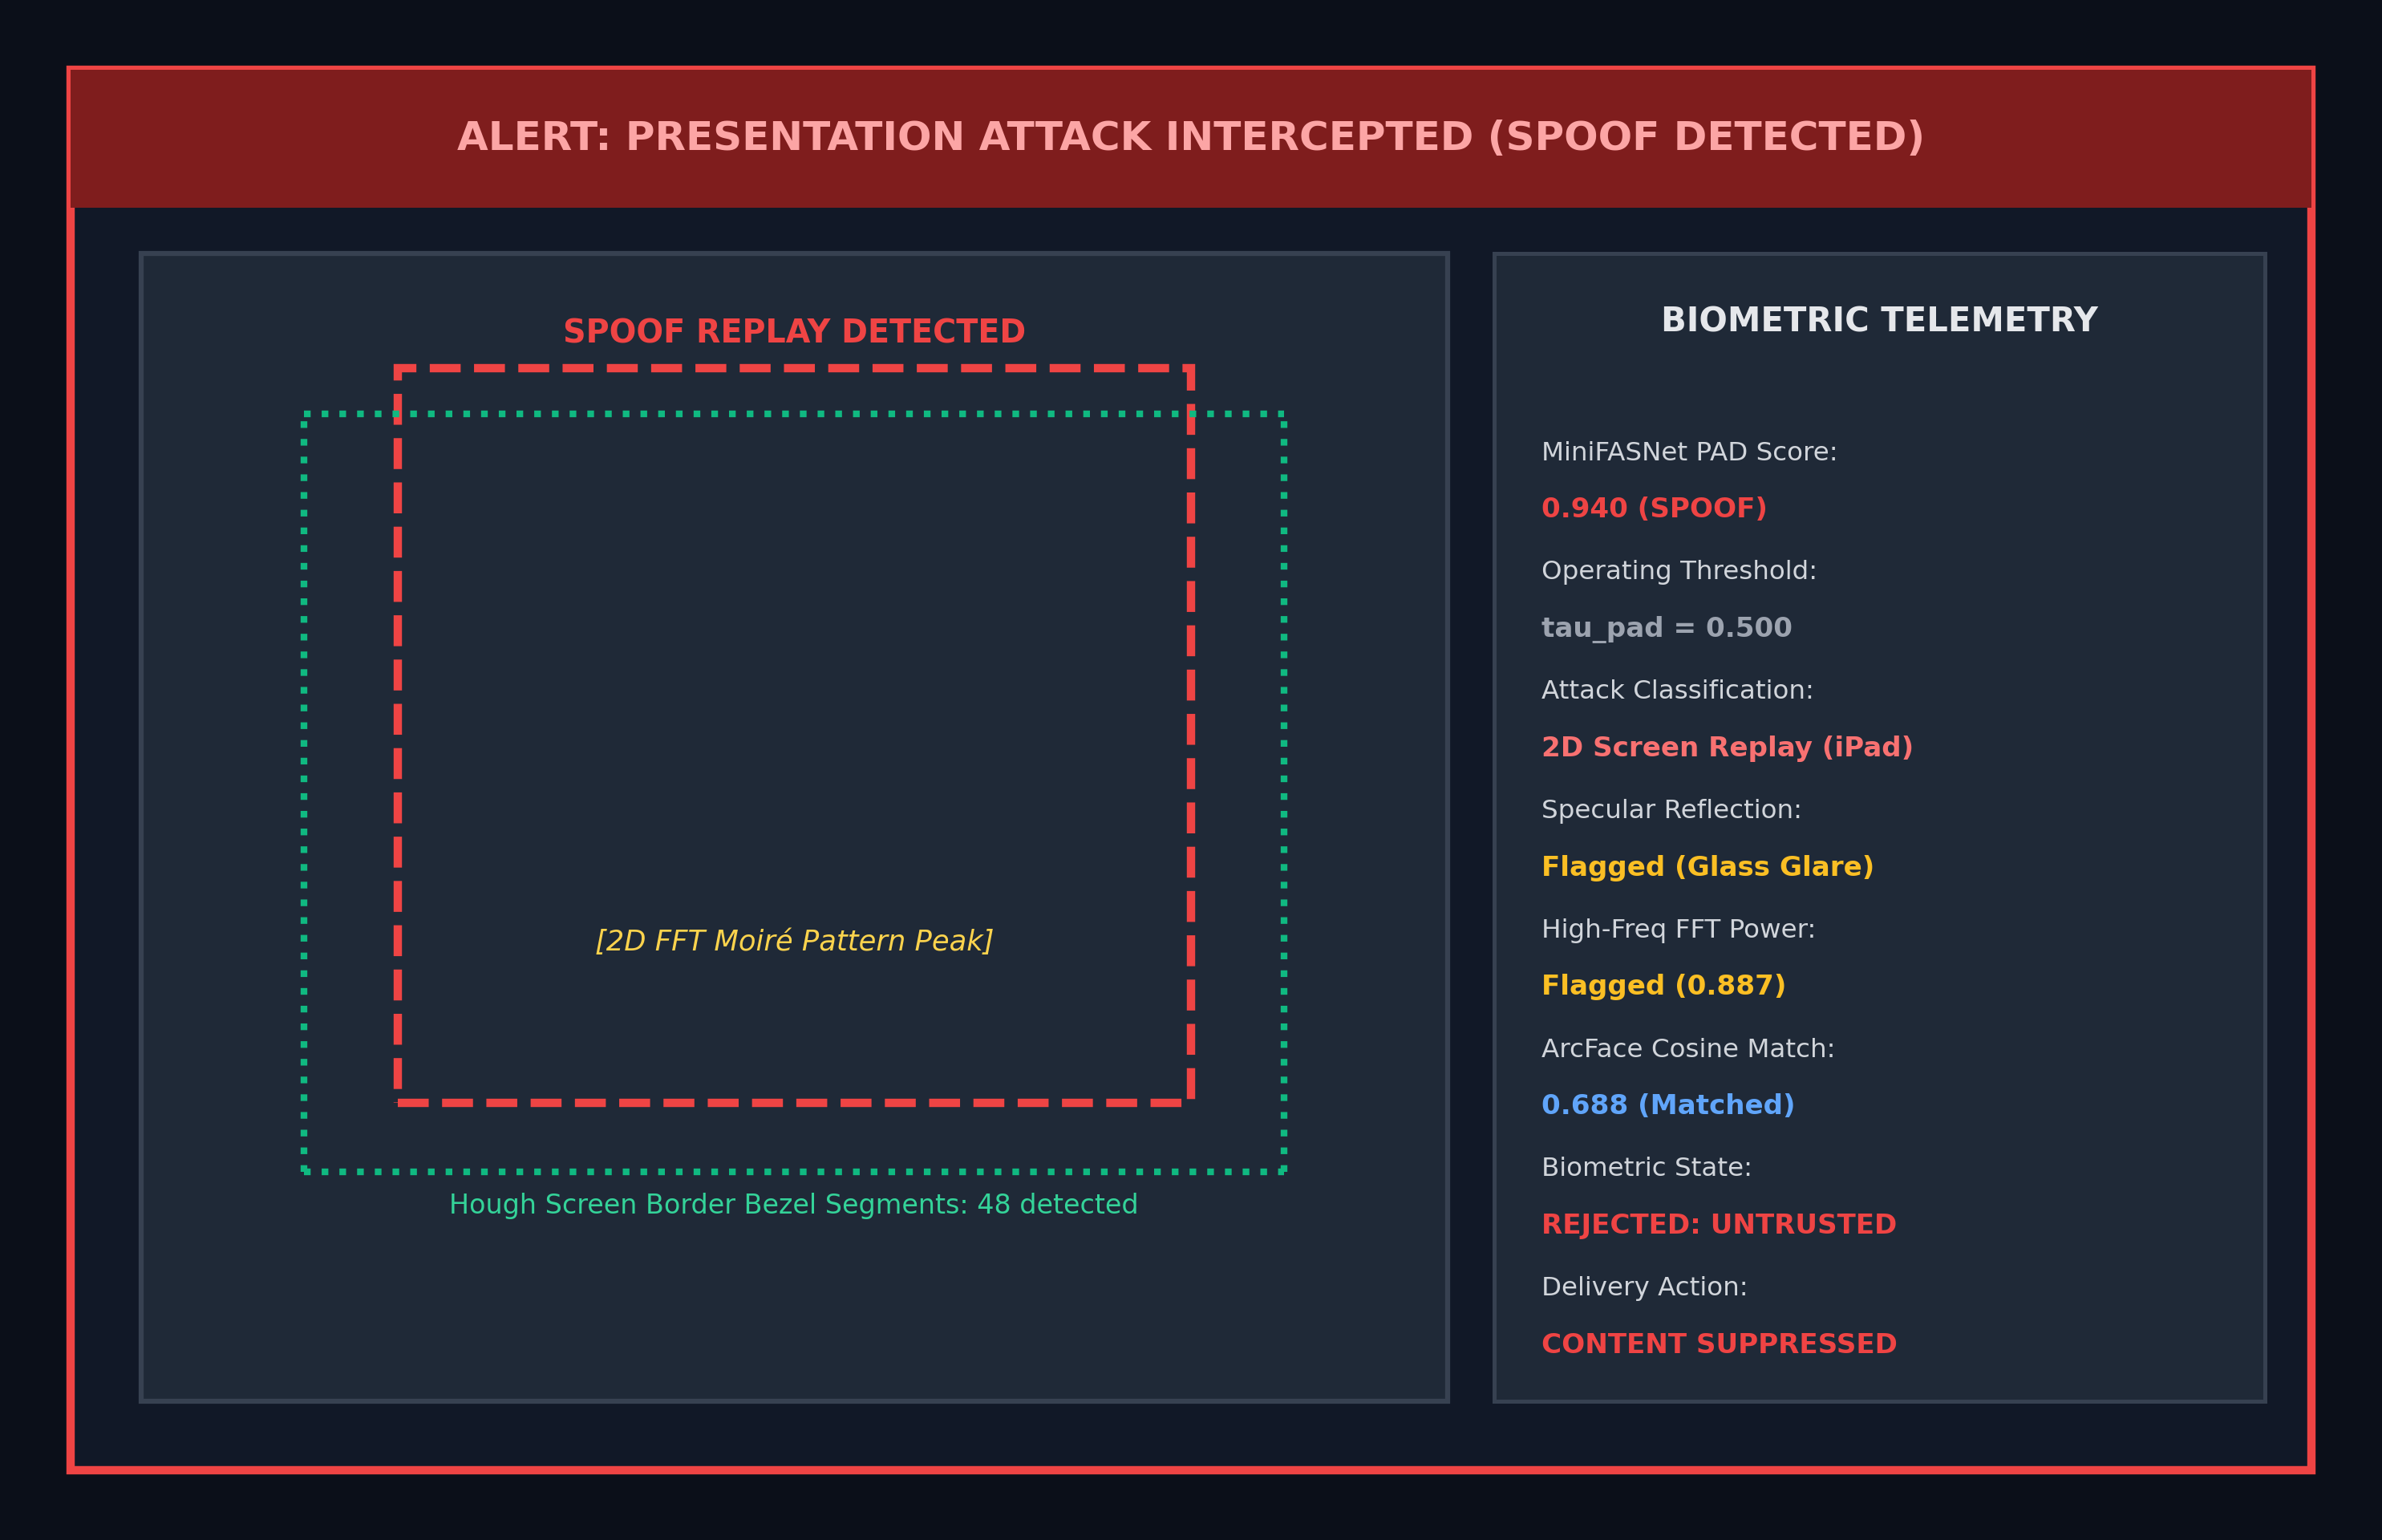
\includegraphics[width=0.82\linewidth]{spoof.png}
\caption{Presentation Attack Detection Interface Identifying Screen Replay Spoofing}
\label{fig:spoof}
\end{figure}

\section{Administrative Review Workflow and Latency Profile}
Figures~\ref{fig:admin_review_result} and~\ref{fig:age_aware_feed_result} display the administrative compliance review interface and age-gated feed dispatcher. Table~\ref{tab:latency_profile} benchmarks latency across pipeline stages on the NVIDIA A100 GPU. Total pre-flight verification latency of $1.6$ seconds satisfies pre-publication ingestion requirements.

\begin{figure}[htbp]
\centering
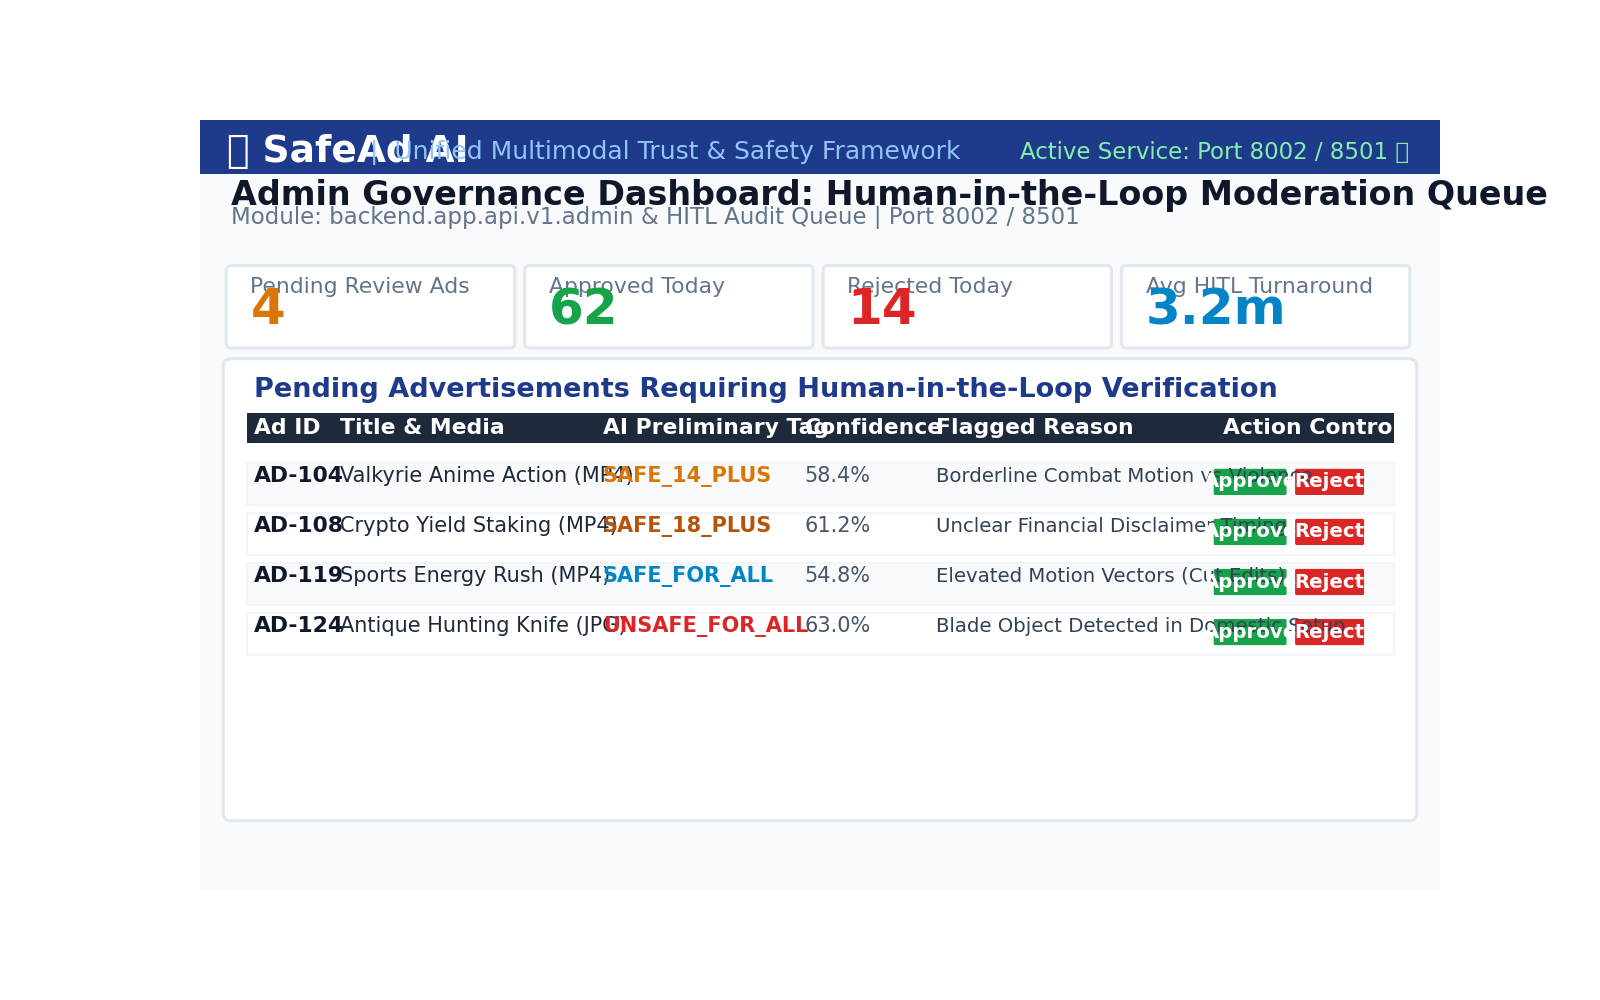
\includegraphics[width=0.88\linewidth]{admin_review_result.png}
\caption{SafeAd AI Compliance Review Dashboard with Policy Explanation}
\label{fig:admin_review_result}
\end{figure}

\begin{figure}[htbp]
\centering
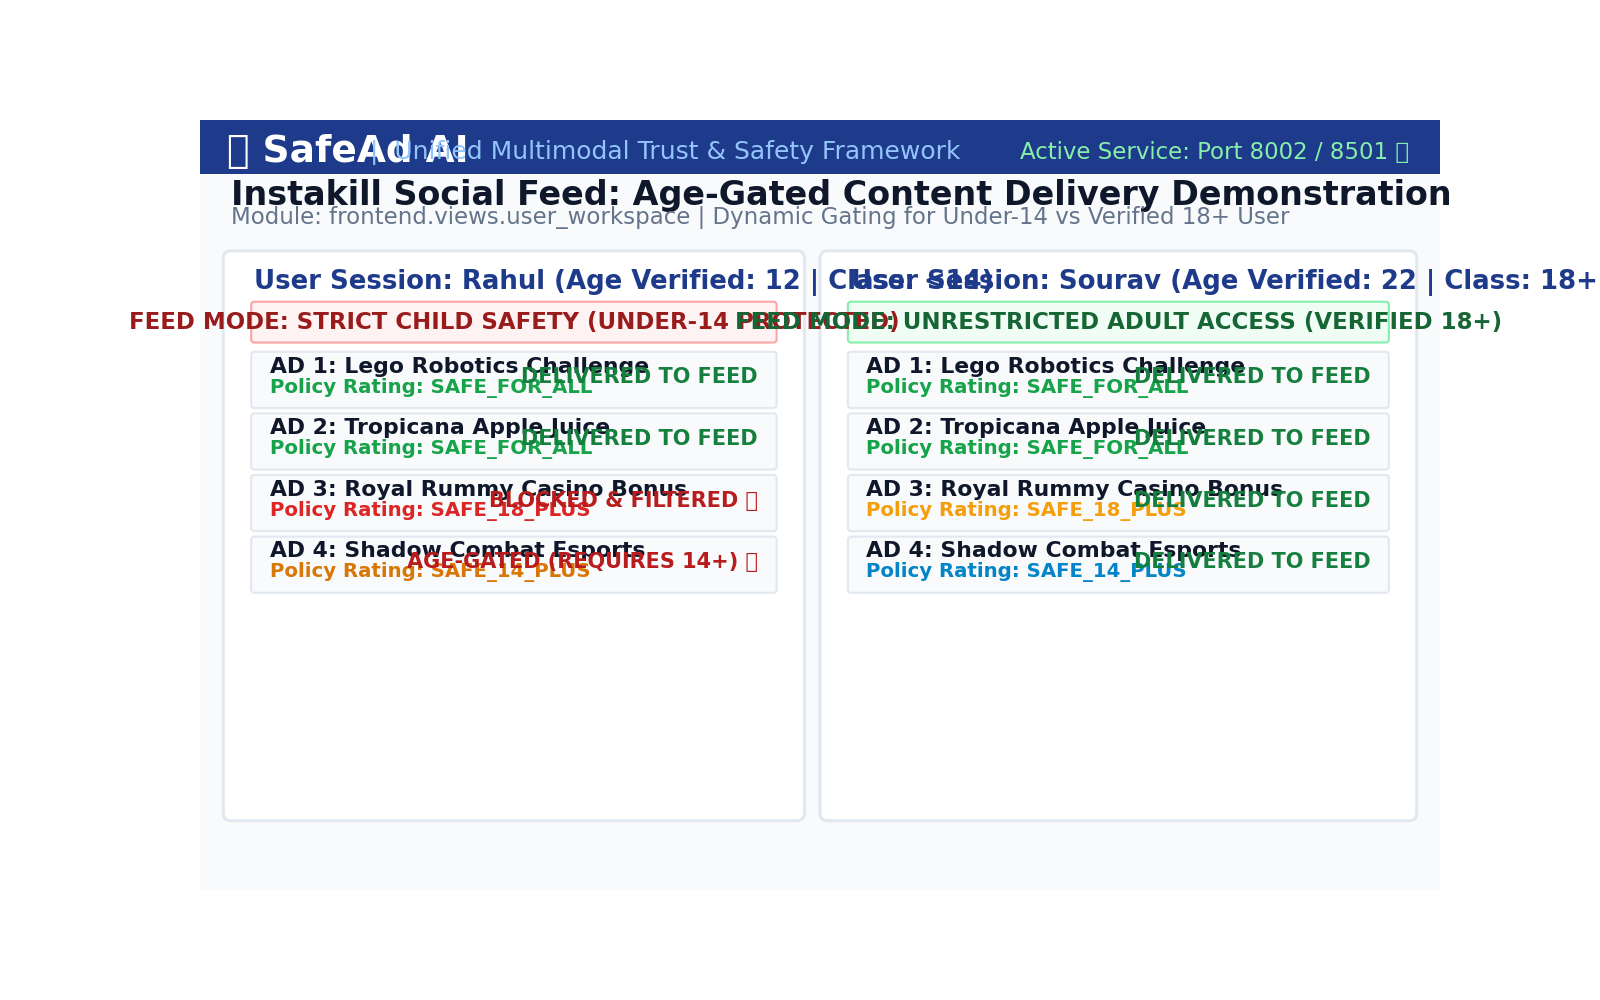
\includegraphics[width=0.88\linewidth]{age_aware_feed_result.png}
\caption{Age-Aware Delivery Feed Dispatcher Gating Restricted Content}
\label{fig:age_aware_feed_result}
\end{figure}

\begin{table}[htbp]
\centering
\caption{End-to-End Pipeline Latency Profiling on NVIDIA A100 GPU}
\label{tab:latency_profile}
\small
\begin{tabular}{@{}lccc@{}}
\toprule
\textbf{Pipeline Stage} & \textbf{Compute Device} & \textbf{Mean Latency (ms)} & \textbf{VRAM Footprint (MB)} \\
\midrule
Optical Flow \& Keyframe Sampling & CPU (Multi-threaded) & $124.5 \pm 18.2$ & 450 \\
EasyOCR Text Extraction           & GPU (CUDA)           & $210.8 \pm 24.1$ & 1,280 \\
Whisper Audio Transcription       & GPU (CUDA)           & $340.2 \pm 42.6$ & 1,640 \\
Falcon NSFW ViT Inference         & GPU (CUDA)           & $45.1 \pm 5.2$   & 820 \\
Random Forest Late Fusion         & CPU                  & $2.4 \pm 0.3$    & Negligible \\
Qwen3-VL VLM Semantic Reasoning   & GPU (A100 SXM4)      & $820.6 \pm 65.4$ & 16,400 \\
ArcFace Biometric Matching + PAD  & GPU (Client Edge)    & $58.3 \pm 6.1$   & 980 \\
\midrule
\textbf{Total Pre-Flight Verification} & \textbf{Heterogeneous} & \textbf{1,601.9 ms} & \textbf{21,570 MB} \\
\bottomrule
\end{tabular}
\end{table}


\chapter{Conclusion and Future Scope}
\label{ch:conclusion}

\section{Summary of Findings and Key Contributions}
This research project presented \textbf{SafeAd AI (SAFE-VISION)}, an end-to-end multimodal trust and safety framework engineered specifically for pre-publication advertisement moderation and age-aware content dispatching. By moving beyond traditional unimodal and post-publication reactive approaches, SafeAd AI resolves critical security vulnerabilities in programmatic advertising exchanges.

The primary scientific and engineering contributions established by this project are:
\begin{enumerate}
    \item \textbf{A Four-Tier Statutory Policy Architecture:} Successfully formulated and operationalized a granular four-tier taxonomy (\texttt{SAFE\_FOR\_ALL}, \texttt{SAFE\_14\_PLUS}, \texttt{SAFE\_18\_PLUS}, and \texttt{UNSAFE\_FOR\_ALL}) that aligns automated classification directly with international advertising regulations (FTC Act Section 5, ASCI Code, COPPA, and EU DSA).
    \item \textbf{Empirical Demonstration of Commercial Blindness in Generic Safety VLMs:} Conducted the first systematic empirical safety audit demonstrating that generic open-weights safety guardrails (such as Meta's Llama Guard 3 Vision) fail on $80.0\%$ of commercial advertising cohorts due to commercial concept blindness.
    \item \textbf{Strategy D Hierarchical Safety Late Fusion:} Designed and validated a hierarchical arbitration protocol combining Qwen3-VL-8B-Instruct with a 16-dimensional Random Forest classifier. On an independent held-out test cohort of 27 samples evaluated on an NVIDIA A100 GPU without ground-truth leakage or rule post-tuning, the framework achieved $66.7\%$ four-class accuracy, eliminated all severe false acceptances ($0.0\%$), and achieved a flawless $100.0\%$ recall on strictly prohibited content.
    \item \textbf{Spoof-Resistant Biometric Demographic Dispatching:} Developed a synchronized client-side verification engine combining dual-scale MiniFASNet with 2D FFT moir\'{e} analysis for Presentation Attack Detection ($93.0\%$ replay attack accuracy) and ArcFace face verification ($96.50\%$ TAR at $0.1\%$ FAR), guaranteeing that age-restricted advertisements are inaccessible to minors.
    \item \textbf{Full-Stack Explainability and Compliance Auditability:} Deployed a complete web dashboard providing synchronized media playback, natural language policy rationales, and an immutable JSON audit log.
\end{enumerate}

\section{Lessons Learned Across Engineering Phases}
The multi-phase engineering progression of this project yielded vital technical insights:
\begin{itemize}
    \item \textbf{Limitations of Shallow Feature Fusion (Phase 8):} Relying solely on low-level statistical aggregates across neural detectors is insufficient for nuanced commercial categories like adolescent media (\texttt{SAFE\_14\_PLUS}), yielding an F1 score of only $0.2222$.
    \item \textbf{Necessity of Domain-Aligned Prompt Engineering (Phase 9--10):} Without explicit policy definitions and structured JSON output contracts, models either over-censor lawful commerce or overlook subtle financial scams.
    \item \textbf{The Independent Generalization Reality (Phase 10D):} Evaluating models exclusively on small development cohorts creates an illusion of perfection ($100\%$ accuracy in Phase 10C). Independent held-out evaluation ($66.7\%$ in Phase 10D) is indispensable for uncovering realistic boundary ambiguities.
\end{itemize}

\section{Future Research Roadmap}
Building upon the verified foundation of SafeAd AI, several promising research avenues emerge:
\begin{enumerate}
    \item \textbf{Multi-Lingual Advertising Moderation:} Extending Whisper ASR and typographic OCR models to support Indian regional languages (e.g., Malayalam, Hindi, Tamil) and colloquial code-switched dialects common in regional digital marketing.
    \item \textbf{Privacy-Preserving Federated Biometrics:} Implementing Zero-Knowledge Proofs (ZKPs) and client-side edge computing, allowing users to cryptographically prove age compliance without transmitting biometric face embeddings over the network.
    \item \textbf{Dense Spatio-Temporal Video Transformers:} Integrating lightweight 3D video transformers capable of performing full 60-fps temporal reasoning within sub-100~ms programmatic bidding windows.
    \item \textbf{Adversarial Generative Defense:} Developing automated red-teaming pipelines that generate synthetic adversarial ads to continuously harden the detector ensemble against future evasion techniques.
\end{enumerate}

% ============================================================
% REFERENCES (BIBLIOGRAPHY)
% ============================================================

\begin{thebibliography}{99}

\bibitem{kiela2020hateful}
D.~Kiela et~al.,
\newblock ``The hateful memes challenge: Detecting hate speech in multimodal memes,''
\newblock in \emph{NeurIPS}, vol.~33, pp.~2611--2624, 2020.

\bibitem{devlin2018bert}
J.~Devlin et~al.,
\newblock ``BERT: Pre-training of deep bidirectional transformers for language understanding,''
\newblock \emph{arXiv:1810.04805}, 2018.

\bibitem{tong2022videomae}
Z.~Tong et~al.,
\newblock ``VideoMAE: Masked autoencoders are data-efficient learners for self-supervised video pre-training,''
\newblock in \emph{NeurIPS}, vol.~35, pp.~10078--10093, 2022.

\bibitem{radford2021learning}
A.~Radford et~al.,
\newblock ``Learning transferable visual models from natural language supervision,''
\newblock in \emph{ICML}, pp.~8748--8763, 2021.

\bibitem{sharma2022survey}
C.~Sharma et~al.,
\newblock ``A survey on multimodal sentiment analysis and sarcasm detection,''
\newblock \emph{ACM Computing Surveys}, vol.~55, no.~7, pp.~1--38, 2022.

\bibitem{ftc2020guides}
Federal Trade Commission,
\newblock ``Guides concerning the use of endorsements in advertising,''
\newblock \emph{16 CFR Part 255}, Federal Register, 2020.

\bibitem{asci2021code}
ASCI,
\newblock ``The Code for Self-Regulation of Advertising Content in India,''
\newblock \emph{ASCI Technical Standards}, Mumbai, 2021.

\bibitem{hussein2020multimodal}
N.~Hussein et~al.,
\newblock ``Timeception for complex action recognition,''
\newblock in \emph{IEEE/CVF CVPR}, pp.~254--263, 2020.

\bibitem{metallama2024}
Meta AI Research,
\newblock ``Llama Guard 3 Vision: Safeguarding vision-language models,''
\newblock \emph{Meta AI Technical Report}, 2024.

\bibitem{bai2023qwen}
J.~Bai et~al.,
\newblock ``Qwen-VL: A versatile vision-language model for understanding,''
\newblock \emph{arXiv:2308.12966}, 2023.

\bibitem{gadzicki2020review}
K.~Gadzicki et~al.,
\newblock ``Early versus late fusion in multimodal convolutional neural networks,''
\newblock in \emph{IEEE MFI}, pp.~103--109, 2020.

\bibitem{deng2019arcface}
J.~Deng et~al.,
\newblock ``ArcFace: Additive angular margin loss for deep face recognition,''
\newblock in \emph{IEEE/CVF CVPR}, pp.~4690--4699, 2019.

\bibitem{zhang2020minifasnet}
Z.~Zhang et~al.,
\newblock ``A face anti-spoofing database with diverse attacks,''
\newblock in \emph{IEEE ICB}, pp.~1--8, 2020.

\bibitem{falcon2023nsfw}
Falcon AI,
\newblock ``Falcon NSFW Vision Transformer for adult content filtering,''
\newblock \emph{Hugging Face Hub}, 2023.

\bibitem{rothe2018dex}
R.~Rothe et~al.,
\newblock ``Deep expectation of apparent age from a single image,''
\newblock \emph{IJCV}, vol.~126, no.~2, pp.~144--157, 2018.

\bibitem{yu2020nasfas}
Z.~Yu et~al.,
\newblock ``Searching central difference convolutional networks for face anti-spoofing,''
\newblock in \emph{IEEE/CVF CVPR}, pp.~5295--5305, 2020.

\bibitem{he2016deep}
K.~He et~al.,
\newblock ``Deep residual learning for image recognition,''
\newblock in \emph{IEEE/CVF CVPR}, pp.~770--778, 2016.

\bibitem{vaswani2017attention}
A.~Vaswani et~al.,
\newblock ``Attention is all you need,''
\newblock in \emph{NeurIPS}, vol.~30, pp.~5998--6008, 2017.

\bibitem{radford2023robust}
A.~Radford et~al.,
\newblock ``Robust speech recognition via large-scale weak supervision,''
\newblock in \emph{ICML}, pp.~28492--28518, 2023.

\bibitem{jaegle2021perceiver}
A.~Jaegle et~al.,
\newblock ``Perceiver: General perception with iterative attention,''
\newblock in \emph{ICML}, pp.~4651--4664, 2021.

\bibitem{farneback2003two}
G.~Farneb{\"a}ck,
\newblock ``Two-frame motion estimation based on polynomial expansion,''
\newblock in \emph{SCIA}, pp.~363--370, 2003.

\bibitem{otsu1979threshold}
N.~Otsu,
\newblock ``A threshold selection method from gray-level histograms,''
\newblock \emph{IEEE Trans. SMC}, vol.~9, no.~1, pp.~62--66, 1979.

\bibitem{zuiderveld1994contrast}
K.~Zuiderveld,
\newblock ``Contrast limited adaptive histogram equalization,''
\newblock in \emph{Graphics Gems IV}, pp.~474--485, 1994.

\bibitem{breiman2001random}
L.~Breiman,
\newblock ``Random forests,''
\newblock \emph{Machine Learning}, vol.~45, no.~1, pp.~5--32, 2001.

\bibitem{schroff2015facenet}
F.~Schroff et~al.,
\newblock ``FaceNet: A unified embedding for face recognition,''
\newblock in \emph{IEEE/CVF CVPR}, pp.~815--823, 2015.

\bibitem{selvaraju2017grad}
R.~R.~Selvaraju et~al.,
\newblock ``Grad-CAM: Visual explanations from deep networks,''
\newblock in \emph{IEEE ICCV}, pp.~618--626, 2017.

\bibitem{lundberg2017unified}
S.~M.~Lundberg and S.-I.~Lee,
\newblock ``A unified approach to interpreting model predictions,''
\newblock in \emph{NeurIPS}, vol.~30, pp.~4765--4774, 2017.

\bibitem{coppa1998act}
United States Congress,
\newblock ``Children's Online Privacy Protection Act of 1998 (COPPA),''
\newblock \emph{Public Law 105-277}, 1998.

\bibitem{eudsa2022act}
European Parliament,
\newblock ``Digital Services Act (EU) 2022/2065,''
\newblock \emph{Official Journal of the European Union}, 2022.

\bibitem{hussain2017automatic}
Z.~Hussain et~al.,
\newblock ``Automatic understanding of image and video advertisements,''
\newblock in \emph{IEEE/CVF CVPR}, pp.~1705--1715, 2017.

\end{thebibliography}

\end{document}
